\documentclass[11pt]{article}
\usepackage[margin=1.1in]{geometry}
\usepackage{booktabs}
\usepackage{amsmath}
\usepackage{graphicx}
\usepackage{xcolor}
% Paper chrome uses the firm-microsim template blue (YGTemplate MyBlue);
% figures use the PolicyEngine palette separately.
\definecolor{paperblue}{rgb}{0,0,0.7}   % MyBlue, matching the sister paper
\definecolor{peteal}{HTML}{39C6C0}      % PolicyEngine teal accent
\usepackage{sectsty}
\allsectionsfont{\color{paperblue}}
\usepackage[colorlinks=true, citecolor=paperblue, linkcolor=paperblue, urlcolor=paperblue]{hyperref}
\usepackage[hang,flushmargin]{footmisc}
\usepackage{natbib}
\bibliographystyle{apalike}
% values_generated.tex — machine-generated by analysis/emit_tex_values.py
% generated 2026-08-27T09:07:33Z from canonical files under results/ (central scenario: realised_2026).
% DO NOT EDIT BY HAND.
% \GENMISSING marks values whose canonical source was absent or is not computable from this dataset; it errors at LaTeX build time by design.
% \GENMISSING errors at build time; run without --draft.
\newcommand{\GENMISSING}{\errmessage{emit_tex_values: missing canonical result}}

\newcommand{\genCentralLossMean}{275}
\newcommand{\genCentralLossPctIncome}{0.60}
\newcommand{\genDecileOneLossGbp}{231}
\newcommand{\genDecileOneLossPct}{2.29}
\newcommand{\genDecileTenLossGbp}{314}
\newcommand{\genDecileTenLossPct}{0.25}
\newcommand{\genDecileRatioPct}{9.2}
\newcommand{\genBetweenDecileRangePct}{2.04}
\newcommand{\genWithinDecileRangePct}{2.79}
\newcommand{\genWithinDecileRangeExDOnePct}{1.98}
\newcommand{\genWithinDecileMedianRangePct}{1.01}
\newcommand{\genWithinDecileMedianOfRangesPct}{2.07}
\newcommand{\genDecileOneRangePct}{10.13}
\newcommand{\genWithinDecileRangeMinExDOnePct}{0.94}
\newcommand{\genWithinDecileRangeMaxExDOnePct}{2.80}
\newcommand{\genDecilesBelowBetweenRange}{five}
\newcommand{\genWithinExceedsBetween}{does}
\newcommand{\genWithinExceedsBetweenExDOne}{does not}
\newcommand{\genBetweenDecileRangeDispersionPct}{2.04}
\newcommand{\genDomesticOnlyDecileRatioPct}{9.31}
\newcommand{\genDomesticOnlyDecileRatioGbp}{0.70}
\newcommand{\genAllChannelDecileRatioPct}{9.22}
\newcommand{\genDomesticOnlyDecileOneLossGbp}{54}
\newcommand{\genDomesticOnlyDecileOneLossPct}{0.57}
\newcommand{\genDomesticOnlyDecileTenLossGbp}{78}
\newcommand{\genDomesticOnlyDecileTenLossPct}{0.06}
\newcommand{\genDomesticOnlyRatioMin}{9.31}
\newcommand{\genDomesticOnlyRatioMax}{9.31}
\newcommand{\genDomesticOnlyRatioSpread}{0.000}
\newcommand{\genDomesticOnlyRatioUnequiv}{5.38}
\newcommand{\genDomesticOnlyRatioEquivSpecCount}{six}
\newcommand{\genSpecificationCount}{seven}
\newcommand{\genDecileRankAgreementPct}{53}
\newcommand{\genDecileRankAgreementUnequivPct}{29}
\newcommand{\genDecileRankAgreementEquivBhcPct}{52}
\newcommand{\genDecileRankMeanGap}{0.57}
\newcommand{\genDecileRankMatchesDenominator}{does}
\newcommand{\genRawCashDecileOneGbp}{231}
\newcommand{\genRawCashDecileTwoGbp}{167}
\newcommand{\genRawCashDecileThreeGbp}{196}
\newcommand{\genRawCashDecileFourGbp}{241}
\newcommand{\genRawCashDecileFiveGbp}{272}
\newcommand{\genRawCashDecileSixGbp}{232}
\newcommand{\genRawCashDecileSevenGbp}{278}
\newcommand{\genRawCashDecileEightGbp}{449}
\newcommand{\genRawCashDecileNineGbp}{372}
\newcommand{\genRawCashDecileTenGbp}{314}
\newcommand{\genRawCashPeakDecile}{eight}
\newcommand{\genRawCashPeakDecileNum}{8}
\newcommand{\genRawCashMonotone}{is not}
\newcommand{\genRawCashMonotoneWord}{non-monotone}
\newcommand{\genRawCashDecileOneOverTen}{0.74}
\newcommand{\genRawCashFallsAtDecileCount}{four}
\newcommand{\genOnsShapeCashDecileOneGbp}{140}
\newcommand{\genOnsShapeCashDecileTwoGbp}{148}
\newcommand{\genOnsShapeCashDecileThreeGbp}{176}
\newcommand{\genOnsShapeCashDecileFourGbp}{205}
\newcommand{\genOnsShapeCashDecileFiveGbp}{235}
\newcommand{\genOnsShapeCashDecileSixGbp}{257}
\newcommand{\genOnsShapeCashDecileSevenGbp}{302}
\newcommand{\genOnsShapeCashDecileEightGbp}{378}
\newcommand{\genOnsShapeCashDecileNineGbp}{423}
\newcommand{\genOnsShapeCashDecileTenGbp}{473}
\newcommand{\genOnsShapeCashPeakDecile}{ten}
\newcommand{\genOnsShapeCashPeakDecileNum}{10}
\newcommand{\genOnsShapeCashMonotone}{is}
\newcommand{\genOnsShapeCashMonotoneWord}{monotone}
\newcommand{\genOnsShapeCashDecileOneOverTen}{0.30}
\newcommand{\genOnsShapeCashFallsAtDecileCount}{zero}
\newcommand{\genOnsLevelsCashDecileOneGbp}{140}
\newcommand{\genOnsLevelsCashDecileTwoGbp}{146}
\newcommand{\genOnsLevelsCashDecileThreeGbp}{171}
\newcommand{\genOnsLevelsCashDecileFourGbp}{199}
\newcommand{\genOnsLevelsCashDecileFiveGbp}{222}
\newcommand{\genOnsLevelsCashDecileSixGbp}{238}
\newcommand{\genOnsLevelsCashDecileSevenGbp}{275}
\newcommand{\genOnsLevelsCashDecileEightGbp}{347}
\newcommand{\genOnsLevelsCashDecileNineGbp}{379}
\newcommand{\genOnsLevelsCashDecileTenGbp}{417}
\newcommand{\genOnsLevelsCashPeakDecile}{ten}
\newcommand{\genOnsLevelsCashPeakDecileNum}{10}
\newcommand{\genOnsLevelsCashMonotone}{is}
\newcommand{\genOnsLevelsCashMonotoneWord}{monotone}
\newcommand{\genOnsLevelsCashDecileOneOverTen}{0.34}
\newcommand{\genOnsLevelsCashFallsAtDecileCount}{zero}
\newcommand{\genCashProfileMonotoneCount}{two}
\newcommand{\genGridReconRatioMin}{9.31}
\newcommand{\genGridReconRatioMax}{9.31}
\newcommand{\genGridReconTolerancePct}{5}
\newcommand{\genGridReconBandLow}{8.85}
\newcommand{\genGridReconBandHigh}{9.78}
\newcommand{\genGridReconScenarioCount}{five}
\newcommand{\genGridReconAllInside}{every}
\newcommand{\genGridReconOutsideCount}{zero}
\newcommand{\genGridReconDomesticOnlyMin}{9.31}
\newcommand{\genGridReconDomesticOnlyMax}{9.31}
\newcommand{\genAggSpendRealisedBn}{8.1}
\newcommand{\genAggSpendAdverseBn}{19.7}
\newcommand{\genAggSpendBaselineBn}{8.7}
\newcommand{\genGasPeakPence}{78}
\newcommand{\genOilPeakUsd}{42}
\newcommand{\genOilPeakPct}{57}
\newcommand{\genGasUnitRatePct}{7.8}
\newcommand{\genElecUnitRatePct}{5.1}
\newcommand{\genCapAnnualised}{1768}
\newcommand{\genCapBaselineLevel}{1663}
\newcommand{\genSocialTariffCostBn}{1.2}
\newcommand{\genSocialTariffShareBottomThree}{57}
\newcommand{\genSocialTariffUncompensatedShare}{84}
\newcommand{\genJrfCostBn}{7.0}
\newcommand{\genJrfShareBottomThree}{31}
\newcommand{\genJrfUncompensatedShare}{24}
\newcommand{\genWhdCostBn}{0.7}
\newcommand{\genWhdShareBottomThree}{60}
\newcommand{\genWhdUncompensatedShare}{86}
\newcommand{\genVatCutCostBn}{2.0}
\newcommand{\genVatCutShareBottomThree}{25}
\newcommand{\genVatCutUncompensatedShare}{85}
\newcommand{\genRebateCostBn}{5.4}
\newcommand{\genRebateShareBottomThree}{30}
\newcommand{\genRebateUncompensatedShare}{32}
\newcommand{\genSocialTariffCostPerPound}{5.81}
\newcommand{\genJrfCostPerPound}{9.98}
\newcommand{\genWhdCostPerPound}{5.11}
\newcommand{\genVatCutCostPerPound}{12.98}
\newcommand{\genRebateCostPerPound}{10.53}
\newcommand{\genBestCostPerPound}{5.11}
\newcommand{\genWorstCostPerPound}{12.98}
\newcommand{\genMotorFuelShareOfLoss}{75.6}
\newcommand{\genGasShareOfLoss}{13.3}
\newcommand{\genElecShareOfLoss}{11.1}
\newcommand{\genDomesticShareOfLoss}{24.4}
\newcommand{\genMotorFuelShareOfLossAdverse}{71.0}
\newcommand{\genGasShareOfLossAdverse}{15.8}
\newcommand{\genElecShareOfLossAdverse}{13.2}
\newcommand{\genDomesticShareOfLossAdverse}{29.0}
\newcommand{\genMainAggBn}{8.1}
\newcommand{\genMainLossMean}{275}
\newcommand{\genMainLossPctIncome}{0.60}
\newcommand{\genMainDecileOneLossGbp}{231}
\newcommand{\genMainDecileOneLossPct}{2.29}
\newcommand{\genMainDecileTenLossGbp}{314}
\newcommand{\genMainDecileTenLossPct}{0.25}
\newcommand{\genMainDecileRatioPct}{9.2}
\newcommand{\genMainMotorFuelShareOfLoss}{75.6}
\newcommand{\genMainGasShareOfLoss}{13.3}
\newcommand{\genMainElecShareOfLoss}{11.1}
\newcommand{\genMainDomesticShareOfLoss}{24.4}
\newcommand{\genSteadyStateAggBn}{8.6}
\newcommand{\genSteadyStateLossMean}{292}
\newcommand{\genSteadyStateLossPctIncome}{0.64}
\newcommand{\genSteadyStateDecileOneLossGbp}{245}
\newcommand{\genSteadyStateDecileOneLossPct}{2.44}
\newcommand{\genSteadyStateDecileTenLossGbp}{333}
\newcommand{\genSteadyStateDecileTenLossPct}{0.26}
\newcommand{\genSteadyStateDecileRatioPct}{9.2}
\newcommand{\genSteadyStateMotorFuelShareOfLoss}{71.3}
\newcommand{\genSteadyStateGasShareOfLoss}{15.7}
\newcommand{\genSteadyStateElecShareOfLoss}{13.1}
\newcommand{\genSteadyStateDomesticShareOfLoss}{28.7}
\newcommand{\genSymDampAggBn}{12.6}
\newcommand{\genSymDampLossMean}{427}
\newcommand{\genSymDampLossPctIncome}{0.94}
\newcommand{\genSymDampDecileOneLossGbp}{354}
\newcommand{\genSymDampDecileOneLossPct}{3.59}
\newcommand{\genSymDampDecileTenLossGbp}{490}
\newcommand{\genSymDampDecileTenLossPct}{0.39}
\newcommand{\genSymDampDecileRatioPct}{9.3}
\newcommand{\genSymDampMotorFuelShareOfLoss}{48.7}
\newcommand{\genSymDampGasShareOfLoss}{27.9}
\newcommand{\genSymDampElecShareOfLoss}{23.4}
\newcommand{\genSymDampDomesticShareOfLoss}{51.3}
\newcommand{\genPeakFuelAggBn}{11.4}
\newcommand{\genPeakFuelLossMean}{387}
\newcommand{\genPeakFuelLossPctIncome}{0.85}
\newcommand{\genPeakFuelDecileOneLossGbp}{326}
\newcommand{\genPeakFuelDecileOneLossPct}{3.22}
\newcommand{\genPeakFuelDecileTenLossGbp}{441}
\newcommand{\genPeakFuelDecileTenLossPct}{0.35}
\newcommand{\genPeakFuelDecileRatioPct}{9.2}
\newcommand{\genPeakFuelMotorFuelShareOfLoss}{82.7}
\newcommand{\genPeakFuelGasShareOfLoss}{9.4}
\newcommand{\genPeakFuelElecShareOfLoss}{7.9}
\newcommand{\genPeakFuelDomesticShareOfLoss}{17.3}
\newcommand{\genOnsShapeAggBn}{8.1}
\newcommand{\genOnsShapeLossMean}{276}
\newcommand{\genOnsShapeLossPctIncome}{0.61}
\newcommand{\genOnsShapeDecileOneLossGbp}{140}
\newcommand{\genOnsShapeDecileOneLossPct}{1.41}
\newcommand{\genOnsShapeDecileTenLossGbp}{473}
\newcommand{\genOnsShapeDecileTenLossPct}{0.37}
\newcommand{\genOnsShapeDecileRatioPct}{3.8}
\newcommand{\genOnsShapeMotorFuelShareOfLoss}{75.7}
\newcommand{\genOnsShapeGasShareOfLoss}{13.2}
\newcommand{\genOnsShapeElecShareOfLoss}{11.1}
\newcommand{\genOnsShapeDomesticShareOfLoss}{24.3}
\newcommand{\genOnsLevelsAggBn}{7.5}
\newcommand{\genOnsLevelsLossMean}{255}
\newcommand{\genOnsLevelsLossPctIncome}{0.56}
\newcommand{\genOnsLevelsDecileOneLossGbp}{140}
\newcommand{\genOnsLevelsDecileOneLossPct}{1.43}
\newcommand{\genOnsLevelsDecileTenLossGbp}{417}
\newcommand{\genOnsLevelsDecileTenLossPct}{0.33}
\newcommand{\genOnsLevelsDecileRatioPct}{4.3}
\newcommand{\genOnsLevelsMotorFuelShareOfLoss}{64.9}
\newcommand{\genOnsLevelsGasShareOfLoss}{19.1}
\newcommand{\genOnsLevelsElecShareOfLoss}{16.0}
\newcommand{\genOnsLevelsDomesticShareOfLoss}{35.1}
\newcommand{\genUnequivAggBn}{8.1}
\newcommand{\genUnequivLossMean}{275}
\newcommand{\genUnequivLossPctIncome}{0.45}
\newcommand{\genUnequivDecileOneLossGbp}{231}
\newcommand{\genUnequivDecileOneLossPct}{1.16}
\newcommand{\genUnequivDecileTenLossGbp}{314}
\newcommand{\genUnequivDecileTenLossPct}{0.21}
\newcommand{\genUnequivDecileRatioPct}{5.5}
\newcommand{\genUnequivMotorFuelShareOfLoss}{75.6}
\newcommand{\genUnequivGasShareOfLoss}{13.3}
\newcommand{\genUnequivElecShareOfLoss}{11.1}
\newcommand{\genUnequivDomesticShareOfLoss}{24.4}
\newcommand{\genOnsFuelAggBn}{8.1}
\newcommand{\genOnsFuelLossMean}{276}
\newcommand{\genOnsFuelLossPctIncome}{0.61}
\newcommand{\genOnsFuelDecileOneLossGbp}{140}
\newcommand{\genOnsFuelDecileOneLossPct}{1.41}
\newcommand{\genOnsFuelDecileTenLossGbp}{473}
\newcommand{\genOnsFuelDecileTenLossPct}{0.37}
\newcommand{\genOnsFuelDecileRatioPct}{3.8}
\newcommand{\genOnsFuelMotorFuelShareOfLoss}{75.7}
\newcommand{\genOnsFuelGasShareOfLoss}{13.2}
\newcommand{\genOnsFuelElecShareOfLoss}{11.1}
\newcommand{\genOnsFuelDomesticShareOfLoss}{24.3}
\newcommand{\genSpecCount}{7}
\newcommand{\genCentralAggBn}{8.10}
\newcommand{\genMainAggPreciseBn}{8.10}
\newcommand{\genSteadyStateAggPreciseBn}{8.59}
\newcommand{\genSymDampAggPreciseBn}{12.57}
\newcommand{\genPeakFuelAggPreciseBn}{11.39}
\newcommand{\genOnsShapeAggPreciseBn}{8.13}
\newcommand{\genOnsLevelsAggPreciseBn}{7.52}
\newcommand{\genUnequivAggPreciseBn}{8.10}
\newcommand{\genPumpSustainedFraction}{65}
\newcommand{\genGasSustainedFraction}{20}
\newcommand{\genDecileEightLossGbp}{449}
\newcommand{\genDecileEightLossPct}{0.84}
\newcommand{\genDecileNineLossGbp}{372}
\newcommand{\genDecileNineLossPct}{0.55}
\newcommand{\genDecileOneMedianLossPct}{0.58}
\newcommand{\genDecileTenMedianLossPct}{0.06}
\newcommand{\genMedianDecileRatioPct}{9.7}
\newcommand{\genDecileOnePNinetyLossPct}{10.30}
\newcommand{\genDecileOneShareAboveFivePct}{16.2}
\newcommand{\genDecileOneShareAboveTenPct}{10.5}
\newcommand{\genRegionMaxLossPct}{1.21}
\newcommand{\genRegionMaxLossGbp}{509}
\newcommand{\genRegionMinLossPct}{0.27}
\newcommand{\genRegionMinLossGbp}{173}
\newcommand{\genMeansTestedShareHouseholds}{15.7}
\newcommand{\genMeansTestedSharePct}{15.7}
\newcommand{\genMeansTestedHouseholdsM}{4.6}
\newcommand{\genRebateFullyCompensatedShare}{68}
\newcommand{\genVatCutMaxOffsetPct}{4.76}
\newcommand{\genElasticityAggZeroBn}{8.10}
\newcommand{\genElasticityAggHighBn}{1.53}
\newcommand{\genLabandeiraShortShaved}{27}
\newcommand{\genPriesmannShortShaved}{31}
\newcommand{\genPriesmannDecileRatio}{3.6}
\newcommand{\genCapLagCumulativeBn}{8.59}
\newcommand{\genCapLagCumulativeMean}{292}
\newcommand{\genCapLagAnnualisedLagOne}{280}
\newcommand{\genCapLagAnnualisedLagOneUnanchored}{280}
\newcommand{\genCapLagAnnualisedLagOnePointFive}{275}
\newcommand{\genCapLagAnnualisedLagOnePointFiveUnanchored}{275}
\newcommand{\genCapLagAnnualisedLagTwo}{271}
\newcommand{\genCapLagAnnualisedLagTwoUnanchored}{271}
\newcommand{\genCapLagAnnualisedLagThree}{267}
\newcommand{\genCapLagAnnualisedLagThreeUnanchored}{263}
\newcommand{\genCapLagAnnualisedLagFour}{272}
\newcommand{\genCapLagAnnualisedLagFourUnanchored}{253}
\newcommand{\genCapLagAnnualisedPaper}{275}
\newcommand{\genCapLagPaperQuarters}{1.5}
\newcommand{\genCapLagRangeGbp}{13}
\newcommand{\genCapLagRangeUnanchoredGbp}{27}
\newcommand{\genCapLagSpreadPct}{5}
\newcommand{\genCapLagSpreadUnanchoredPct}{10}
\newcommand{\genMotorFuelAnnualisedBn}{6.1}
\newcommand{\genDomesticAnnualisedBn}{2.0}
\newcommand{\genCalendarAggBn}{7.0}
\newcommand{\genCalendarMotorFuelShareOfLoss}{80}
\newcommand{\genCalendarDomesticBn}{1.4}
\newcommand{\genCalendarMotorFuelBn}{5.6}
\newcommand{\genCalendarPumpFraction}{0.59}
\newcommand{\genAsymMeanLossLow}{269}
\newcommand{\genAsymRatioLow}{9.21}
\newcommand{\genAsymMeanLossHigh}{280}
\newcommand{\genAsymRatioHigh}{9.22}
\newcommand{\genAsymMeanShiftPct}{4.1}
\newcommand{\genGasShareDomesticLow}{59.2}
\newcommand{\genGasShareDomesticCentral}{54.4}
\newcommand{\genGasShareDomesticHigh}{50.4}
\newcommand{\genCvUpperBn}{8.10}
\newcommand{\genCvUpperMeanGbp}{275}
\newcommand{\genCvLowerHighEpsBn}{7.22}
\newcommand{\genCvLowerHighEpsMeanGbp}{245}
\newcommand{\genWelfareShavedHighEpsPct}{10.8}
\newcommand{\genSpendShavedHighEpsPct}{81}
\newcommand{\genWelfareShavedMaxPct}{10.8}
\newcommand{\genCvLowerMinBn}{7.22}
\newcommand{\genLabandeiraShortWelfareShaved}{3.9}
\newcommand{\genLabandeiraShortSpendShaved}{27}
\newcommand{\genLabandeiraShortCvLowerBn}{7.78}
\newcommand{\genPriesmannShortWelfareShaved}{4.0}
\newcommand{\genPriesmannShortSpendShaved}{31}
\newcommand{\genPriesmannShortCvLowerBn}{7.78}
\newcommand{\genSpecAggMinBn}{7.52}
\newcommand{\genSpecAggMaxBn}{12.57}
\newcommand{\genSpecLossMeanMin}{255}
\newcommand{\genSpecLossMeanMax}{427}
\newcommand{\genSpecFuelShareMinPct}{48.7}
\newcommand{\genSpecFuelShareMaxPct}{82.7}
\newcommand{\genSpecDecileRatioMin}{3.75}
\newcommand{\genSpecDecileRatioMax}{9.25}
\newcommand{\genSpecAggSpreadPct}{62}
\newcommand{\genSpecFuelShareMaxExPeakPct}{75.7}
\newcommand{\genAnnualPhaseInGasPct}{79.7}
\newcommand{\genAnnualPhaseInElecPct}{80.3}
\newcommand{\genCoverageExcludedHouseholdsM}{0.24}
\newcommand{\genCoverageExcludedSharePct}{0.81}
\newcommand{\genCoverageExcludedLossSharePct}{0.79}
\newcommand{\genCoverageExcludedZeroIncomeSharePct}{100}
\newcommand{\genCoveredHouseholdsM}{29.23}
\newcommand{\genCoveredLossBn}{8.03}
\newcommand{\genZeroOrNegIncomeSharePct}{3.19}
\newcommand{\genDecileOneZeroIncomeShare}{20.05}
\newcommand{\genDecileOneZeroIncomeShareUnequiv}{0.57}
\newcommand{\genDecileOneMedianIncomeGbp}{7,590}
\newcommand{\genDecileOneMeanIncomeGbp}{5,865}
\newcommand{\genDecileOneMedianIncomeUnequivGbp}{16,000}
\newcommand{\genModelDomesticMeanGbp}{1,331}
\newcommand{\genModelFuelMeanGbp}{1,212}
\newcommand{\genFuelSpendDecileOneRawGbp}{1,073}
\newcommand{\genFuelSpendDecileOneOnsGbp}{521}
\newcommand{\genRescaledFuelDecileOneGbp}{521}
\newcommand{\genOnsLevelsFuelDecileOneGbp}{412}
\newcommand{\genFuelSpendDecileTenRawGbp}{1,333}
\newcommand{\genFuelSpendDecileTenOnsGbp}{2,230}
\newcommand{\genRescaledFuelDecileTenGbp}{2,230}
\newcommand{\genOnsLevelsFuelDecileTenGbp}{1,767}
\newcommand{\genOnsBenchFuelDecileOneGbp}{318}
\newcommand{\genOnsBenchFuelDecileTenGbp}{1,362}
\newcommand{\genOnsBenchFuelMeanGbp}{960}
\newcommand{\genOnsBenchDomesticMeanGbp}{1,780}
\newcommand{\genOnsBenchFuelRatio}{4.3}
\newcommand{\genDomesticUnderImputationPct}{25}
\newcommand{\genFuelOverImputationPct}{26}
\newcommand{\genSocialTariffOffsetSharePct}{3.9}
\newcommand{\genSocialTariffResidualMeanGbp}{264}
\newcommand{\genSocialTariffResidualMedianGbp}{46}
\newcommand{\genSocialTariffResidualDecileOneGbp}{209}
\newcommand{\genSocialTariffResidualDecileTenGbp}{313}
\newcommand{\genSocialTariffOffsetDecileOnePct}{10}
\newcommand{\genSocialTariffMeanGainGbp}{42}
\newcommand{\genSocialTariffFullyCompensatedShare}{16}
\newcommand{\genJrfOffsetSharePct}{40.6}
\newcommand{\genJrfResidualMeanGbp}{163}
\newcommand{\genJrfResidualMedianGbp}{0}
\newcommand{\genJrfResidualDecileOneGbp}{129}
\newcommand{\genJrfResidualDecileTenGbp}{204}
\newcommand{\genJrfOffsetDecileOnePct}{44}
\newcommand{\genJrfMeanGainGbp}{237}
\newcommand{\genJrfFullyCompensatedShare}{76}
\newcommand{\genWhdOffsetSharePct}{2.9}
\newcommand{\genWhdResidualMeanGbp}{267}
\newcommand{\genWhdResidualMedianGbp}{49}
\newcommand{\genWhdResidualDecileOneGbp}{217}
\newcommand{\genWhdResidualDecileTenGbp}{313}
\newcommand{\genWhdOffsetDecileOnePct}{6}
\newcommand{\genWhdMeanGainGbp}{23}
\newcommand{\genWhdFullyCompensatedShare}{14}
\newcommand{\genVatCutOffsetSharePct}{24.2}
\newcommand{\genVatCutResidualMeanGbp}{208}
\newcommand{\genVatCutResidualMedianGbp}{4}
\newcommand{\genVatCutResidualDecileOneGbp}{177}
\newcommand{\genVatCutResidualDecileTenGbp}{237}
\newcommand{\genVatCutOffsetDecileOnePct}{23}
\newcommand{\genVatCutMeanGainGbp}{67}
\newcommand{\genVatCutFullyCompensatedShare}{15}
\newcommand{\genRebateOffsetSharePct}{33.7}
\newcommand{\genRebateResidualMeanGbp}{182}
\newcommand{\genRebateResidualMedianGbp}{0}
\newcommand{\genRebateResidualDecileOneGbp}{149}
\newcommand{\genRebateResidualDecileTenGbp}{221}
\newcommand{\genRebateOffsetDecileOnePct}{36}
\newcommand{\genRebateMeanGainGbp}{183}
\newcommand{\genJrfStatedCostBn}{5.0}
\newcommand{\genJrfCostOverStated}{1.4}
\newcommand{\genEnvelopeBn}{5}
\newcommand{\genSocialTariffStatedParameterPct}{35}
\newcommand{\genSocialTariffStatedParameter}{35}
\newcommand{\genSocialTariffFeasibleMaxParameterPct}{100}
\newcommand{\genSocialTariffFeasibleMaxParameter}{100}
\newcommand{\genSocialTariffAbsorbableBn}{3.50}
\newcommand{\genSocialTariffAbsorbableEnvelopeBn}{3.50}
\newcommand{\genSocialTariffAbsorbsFullEnvelope}{no}
\newcommand{\genSocialTariffCappedOffsetPct}{4.0}
\newcommand{\genSocialTariffCappedCostBn}{3.50}
\newcommand{\genSocialTariffCappedResidualMeanGbp}{264}
\newcommand{\genSocialTariffCappedResidualMedianGbp}{46}
\newcommand{\genSocialTariffCappedResidualDecileOneGbp}{208}
\newcommand{\genSocialTariffCappedMeanGainGbp}{119}
\newcommand{\genSocialTariffCappedUncompensatedPct}{84}
\newcommand{\genSocialTariffCappedShareToBottomThreePct}{57.4}
\newcommand{\genSocialTariffCappedCostPerPound}{5.8}
\newcommand{\genSocialTariffCappedScale}{2.86}
\newcommand{\genSocialTariffCappedParameterPct}{100}
\newcommand{\genSocialTariffCappedParameter}{100}
\newcommand{\genSocialTariffCappedFeasible}{yes}
\newcommand{\genSocialTariffCappedIsFeasible}{feasible}
\newcommand{\genSocialTariffEnvelopeOffsetPct}{4.0}
\newcommand{\genSocialTariffEnvelopeCostBn}{3.50}
\newcommand{\genSocialTariffEnvelopeResidualMeanGbp}{264}
\newcommand{\genSocialTariffEnvelopeResidualMedianGbp}{46}
\newcommand{\genSocialTariffEnvelopeResidualDecileOneGbp}{208}
\newcommand{\genSocialTariffEnvelopeMeanGainGbp}{119}
\newcommand{\genSocialTariffEnvelopeUncompensatedPct}{84}
\newcommand{\genSocialTariffEnvelopeShareToBottomThreePct}{57.4}
\newcommand{\genSocialTariffEnvelopeCostPerPound}{5.8}
\newcommand{\genSocialTariffEnvelopeScale}{2.86}
\newcommand{\genSocialTariffEnvelopeParameterPct}{100}
\newcommand{\genSocialTariffEnvelopeParameter}{100}
\newcommand{\genSocialTariffEnvelopeFeasible}{yes}
\newcommand{\genSocialTariffEnvelopeIsFeasible}{feasible}
\newcommand{\genSocialTariffScaledOffsetPct}{4.0}
\newcommand{\genSocialTariffScaledCostBn}{5.00}
\newcommand{\genSocialTariffScaledResidualMeanGbp}{264}
\newcommand{\genSocialTariffScaledResidualMedianGbp}{46}
\newcommand{\genSocialTariffScaledResidualDecileOneGbp}{208}
\newcommand{\genSocialTariffScaledMeanGainGbp}{170}
\newcommand{\genSocialTariffScaledUncompensatedPct}{84}
\newcommand{\genSocialTariffScaledShareToBottomThreePct}{57.4}
\newcommand{\genSocialTariffScaledCostPerPound}{5.8}
\newcommand{\genSocialTariffScaledScale}{4.08}
\newcommand{\genSocialTariffScaledParameterPct}{143}
\newcommand{\genSocialTariffScaledParameter}{143}
\newcommand{\genSocialTariffScaledFeasible}{no}
\newcommand{\genSocialTariffScaledIsFeasible}{infeasible}
\newcommand{\genSocialTariffEligibilityOffsetPct}{27.6}
\newcommand{\genSocialTariffEligibilityCostBn}{5.00}
\newcommand{\genSocialTariffEligibilityResidualMeanGbp}{199}
\newcommand{\genSocialTariffEligibilityResidualMedianGbp}{24}
\newcommand{\genSocialTariffEligibilityResidualDecileOneGbp}{36}
\newcommand{\genSocialTariffEligibilityMeanGainGbp}{170}
\newcommand{\genSocialTariffEligibilityUncompensatedPct}{59}
\newcommand{\genSocialTariffEligibilityShareToBottomThreePct}{69.0}
\newcommand{\genSocialTariffEligibilityCostPerPound}{4.5}
\newcommand{\genSocialTariffEligibilityScale}{1.00}
\newcommand{\genSocialTariffEligibilityParameterPct}{35}
\newcommand{\genSocialTariffEligibilityParameter}{35}
\newcommand{\genSocialTariffEligibilityFeasible}{yes}
\newcommand{\genSocialTariffEligibilityIsFeasible}{feasible}
\newcommand{\genSocialTariffEligibleSharePct}{42}
\newcommand{\genSocialTariffStatedOffsetPct}{3.9}
\newcommand{\genSocialTariffStatedCostBn}{1.23}
\newcommand{\genSocialTariffStatedResidualMeanGbp}{264}
\newcommand{\genSocialTariffStatedResidualMedianGbp}{46}
\newcommand{\genSocialTariffStatedResidualDecileOneGbp}{209}
\newcommand{\genSocialTariffStatedMeanGainGbp}{42}
\newcommand{\genSocialTariffStatedUncompensatedPct}{84}
\newcommand{\genSocialTariffStatedShareToBottomThreePct}{57.4}
\newcommand{\genSocialTariffStatedCostPerPound}{5.8}
\newcommand{\genSocialTariffStatedScale}{1.00}
\newcommand{\genSocialTariffStatedFeasible}{yes}
\newcommand{\genSocialTariffStatedIsFeasible}{feasible}
\newcommand{\genJrfStatedParameterPct}{50}
\newcommand{\genJrfStatedParameter}{50}
\newcommand{\genJrfFeasibleMaxParameterPct}{100}
\newcommand{\genJrfFeasibleMaxParameter}{100}
\newcommand{\genJrfAbsorbableBn}{5.00}
\newcommand{\genJrfAbsorbableEnvelopeBn}{5.00}
\newcommand{\genJrfAbsorbsFullEnvelope}{yes}
\newcommand{\genJrfCappedOffsetPct}{33.6}
\newcommand{\genJrfCappedCostBn}{5.00}
\newcommand{\genJrfCappedResidualMeanGbp}{182}
\newcommand{\genJrfCappedResidualMedianGbp}{0}
\newcommand{\genJrfCappedResidualDecileOneGbp}{145}
\newcommand{\genJrfCappedMeanGainGbp}{170}
\newcommand{\genJrfCappedUncompensatedPct}{33}
\newcommand{\genJrfCappedShareToBottomThreePct}{31.2}
\newcommand{\genJrfCappedCostPerPound}{10.0}
\newcommand{\genJrfCappedScale}{0.72}
\newcommand{\genJrfCappedParameterPct}{35.8}
\newcommand{\genJrfCappedParameter}{35.8}
\newcommand{\genJrfCappedFeasible}{yes}
\newcommand{\genJrfCappedIsFeasible}{feasible}
\newcommand{\genJrfEnvelopeOffsetPct}{33.6}
\newcommand{\genJrfEnvelopeCostBn}{5.00}
\newcommand{\genJrfEnvelopeResidualMeanGbp}{182}
\newcommand{\genJrfEnvelopeResidualMedianGbp}{0}
\newcommand{\genJrfEnvelopeResidualDecileOneGbp}{145}
\newcommand{\genJrfEnvelopeMeanGainGbp}{170}
\newcommand{\genJrfEnvelopeUncompensatedPct}{33}
\newcommand{\genJrfEnvelopeShareToBottomThreePct}{31.2}
\newcommand{\genJrfEnvelopeCostPerPound}{10.0}
\newcommand{\genJrfEnvelopeScale}{0.72}
\newcommand{\genJrfEnvelopeParameterPct}{35.8}
\newcommand{\genJrfEnvelopeParameter}{35.8}
\newcommand{\genJrfEnvelopeFeasible}{yes}
\newcommand{\genJrfEnvelopeIsFeasible}{feasible}
\newcommand{\genJrfScaledOffsetPct}{33.6}
\newcommand{\genJrfScaledCostBn}{5.00}
\newcommand{\genJrfScaledResidualMeanGbp}{182}
\newcommand{\genJrfScaledResidualMedianGbp}{0}
\newcommand{\genJrfScaledResidualDecileOneGbp}{145}
\newcommand{\genJrfScaledMeanGainGbp}{170}
\newcommand{\genJrfScaledUncompensatedPct}{33}
\newcommand{\genJrfScaledShareToBottomThreePct}{31.2}
\newcommand{\genJrfScaledCostPerPound}{10.0}
\newcommand{\genJrfScaledScale}{0.72}
\newcommand{\genJrfScaledParameterPct}{35.8}
\newcommand{\genJrfScaledParameter}{35.8}
\newcommand{\genJrfScaledFeasible}{yes}
\newcommand{\genJrfScaledIsFeasible}{feasible}
\newcommand{\genJrfStatedOffsetPct}{40.6}
\newcommand{\genJrfStatedResidualMeanGbp}{163}
\newcommand{\genJrfStatedResidualMedianGbp}{0}
\newcommand{\genJrfStatedResidualDecileOneGbp}{129}
\newcommand{\genJrfStatedMeanGainGbp}{237}
\newcommand{\genJrfStatedUncompensatedPct}{24}
\newcommand{\genJrfStatedShareToBottomThreePct}{31.2}
\newcommand{\genJrfStatedCostPerPound}{10.0}
\newcommand{\genJrfStatedScale}{1.00}
\newcommand{\genJrfStatedFeasible}{yes}
\newcommand{\genJrfStatedIsFeasible}{feasible}
\newcommand{\genWhdStatedParameterGbp}{150}
\newcommand{\genWhdStatedParameter}{150}
\newcommand{\genWhdFeasibleMaxParameterGbp}{758}
\newcommand{\genWhdFeasibleMaxParameter}{758}
\newcommand{\genWhdAbsorbableBn}{3.50}
\newcommand{\genWhdAbsorbableEnvelopeBn}{3.50}
\newcommand{\genWhdAbsorbsFullEnvelope}{no}
\newcommand{\genWhdCappedOffsetPct}{3.9}
\newcommand{\genWhdCappedCostBn}{3.50}
\newcommand{\genWhdCappedResidualMeanGbp}{264}
\newcommand{\genWhdCappedResidualMedianGbp}{47}
\newcommand{\genWhdCappedResidualDecileOneGbp}{209}
\newcommand{\genWhdCappedMeanGainGbp}{119}
\newcommand{\genWhdCappedUncompensatedPct}{84}
\newcommand{\genWhdCappedShareToBottomThreePct}{60.0}
\newcommand{\genWhdCappedCostPerPound}{5.1}
\newcommand{\genWhdCappedScale}{5.06}
\newcommand{\genWhdCappedParameterGbp}{758}
\newcommand{\genWhdCappedParameter}{758}
\newcommand{\genWhdCappedFeasible}{yes}
\newcommand{\genWhdCappedIsFeasible}{feasible}
\newcommand{\genWhdEnvelopeOffsetPct}{3.9}
\newcommand{\genWhdEnvelopeCostBn}{3.50}
\newcommand{\genWhdEnvelopeResidualMeanGbp}{264}
\newcommand{\genWhdEnvelopeResidualMedianGbp}{47}
\newcommand{\genWhdEnvelopeResidualDecileOneGbp}{209}
\newcommand{\genWhdEnvelopeMeanGainGbp}{119}
\newcommand{\genWhdEnvelopeUncompensatedPct}{84}
\newcommand{\genWhdEnvelopeShareToBottomThreePct}{60.0}
\newcommand{\genWhdEnvelopeCostPerPound}{5.1}
\newcommand{\genWhdEnvelopeScale}{5.06}
\newcommand{\genWhdEnvelopeParameterGbp}{758}
\newcommand{\genWhdEnvelopeParameter}{758}
\newcommand{\genWhdEnvelopeFeasible}{yes}
\newcommand{\genWhdEnvelopeIsFeasible}{feasible}
\newcommand{\genWhdScaledOffsetPct}{4.0}
\newcommand{\genWhdScaledCostBn}{5.00}
\newcommand{\genWhdScaledResidualMeanGbp}{264}
\newcommand{\genWhdScaledResidualMedianGbp}{46}
\newcommand{\genWhdScaledResidualDecileOneGbp}{208}
\newcommand{\genWhdScaledMeanGainGbp}{170}
\newcommand{\genWhdScaledUncompensatedPct}{84}
\newcommand{\genWhdScaledShareToBottomThreePct}{60.0}
\newcommand{\genWhdScaledCostPerPound}{5.1}
\newcommand{\genWhdScaledScale}{7.22}
\newcommand{\genWhdScaledParameterGbp}{1,083}
\newcommand{\genWhdScaledParameter}{1,083}
\newcommand{\genWhdScaledFeasible}{no}
\newcommand{\genWhdScaledIsFeasible}{infeasible}
\newcommand{\genWhdEligibilityOffsetPct}{29.7}
\newcommand{\genWhdEligibilityCostBn}{4.42}
\newcommand{\genWhdEligibilityResidualMeanGbp}{193}
\newcommand{\genWhdEligibilityResidualMedianGbp}{0}
\newcommand{\genWhdEligibilityResidualDecileOneGbp}{158}
\newcommand{\genWhdEligibilityMeanGainGbp}{150}
\newcommand{\genWhdEligibilityUncompensatedPct}{37}
\newcommand{\genWhdEligibilityShareToBottomThreePct}{30.0}
\newcommand{\genWhdEligibilityCostPerPound}{10.5}
\newcommand{\genWhdEligibilityScale}{1.00}
\newcommand{\genWhdEligibilityParameterGbp}{150}
\newcommand{\genWhdEligibilityParameter}{150}
\newcommand{\genWhdEligibilityFeasible}{yes}
\newcommand{\genWhdEligibilityIsFeasible}{feasible}
\newcommand{\genWhdEligibleSharePct}{100}
\newcommand{\genWhdStatedOffsetPct}{2.9}
\newcommand{\genWhdStatedCostBn}{0.69}
\newcommand{\genWhdStatedResidualMeanGbp}{267}
\newcommand{\genWhdStatedResidualMedianGbp}{49}
\newcommand{\genWhdStatedResidualDecileOneGbp}{217}
\newcommand{\genWhdStatedMeanGainGbp}{23}
\newcommand{\genWhdStatedUncompensatedPct}{86}
\newcommand{\genWhdStatedShareToBottomThreePct}{60.0}
\newcommand{\genWhdStatedCostPerPound}{5.1}
\newcommand{\genWhdStatedScale}{1.00}
\newcommand{\genWhdStatedFeasible}{yes}
\newcommand{\genWhdStatedIsFeasible}{feasible}
\newcommand{\genVatCutStatedParameterPct}{5}
\newcommand{\genVatCutStatedParameter}{5}
\newcommand{\genVatCutFeasibleMaxParameterPct}{5}
\newcommand{\genVatCutFeasibleMaxParameter}{5}
\newcommand{\genVatCutAbsorbableBn}{1.96}
\newcommand{\genVatCutAbsorbableEnvelopeBn}{1.96}
\newcommand{\genVatCutAbsorbsFullEnvelope}{no}
\newcommand{\genVatCutCappedOffsetPct}{24.2}
\newcommand{\genVatCutCappedCostBn}{1.96}
\newcommand{\genVatCutCappedResidualMeanGbp}{208}
\newcommand{\genVatCutCappedResidualMedianGbp}{4}
\newcommand{\genVatCutCappedResidualDecileOneGbp}{177}
\newcommand{\genVatCutCappedMeanGainGbp}{67}
\newcommand{\genVatCutCappedUncompensatedPct}{85}
\newcommand{\genVatCutCappedShareToBottomThreePct}{24.7}
\newcommand{\genVatCutCappedCostPerPound}{13.0}
\newcommand{\genVatCutCappedScale}{1.00}
\newcommand{\genVatCutCappedParameterPct}{5}
\newcommand{\genVatCutCappedParameter}{5}
\newcommand{\genVatCutCappedFeasible}{yes}
\newcommand{\genVatCutCappedIsFeasible}{feasible}
\newcommand{\genVatCutEnvelopeOffsetPct}{24.2}
\newcommand{\genVatCutEnvelopeCostBn}{1.96}
\newcommand{\genVatCutEnvelopeResidualMeanGbp}{208}
\newcommand{\genVatCutEnvelopeResidualMedianGbp}{4}
\newcommand{\genVatCutEnvelopeResidualDecileOneGbp}{177}
\newcommand{\genVatCutEnvelopeMeanGainGbp}{67}
\newcommand{\genVatCutEnvelopeUncompensatedPct}{85}
\newcommand{\genVatCutEnvelopeShareToBottomThreePct}{24.7}
\newcommand{\genVatCutEnvelopeCostPerPound}{13.0}
\newcommand{\genVatCutEnvelopeScale}{1.00}
\newcommand{\genVatCutEnvelopeParameterPct}{5}
\newcommand{\genVatCutEnvelopeParameter}{5}
\newcommand{\genVatCutEnvelopeFeasible}{yes}
\newcommand{\genVatCutEnvelopeIsFeasible}{feasible}
\newcommand{\genVatCutScaledOffsetPct}{50.5}
\newcommand{\genVatCutScaledCostBn}{5.00}
\newcommand{\genVatCutScaledResidualMeanGbp}{136}
\newcommand{\genVatCutScaledResidualMedianGbp}{0}
\newcommand{\genVatCutScaledResidualDecileOneGbp}{123}
\newcommand{\genVatCutScaledMeanGainGbp}{170}
\newcommand{\genVatCutScaledUncompensatedPct}{36}
\newcommand{\genVatCutScaledShareToBottomThreePct}{24.7}
\newcommand{\genVatCutScaledCostPerPound}{13.0}
\newcommand{\genVatCutScaledScale}{2.55}
\newcommand{\genVatCutScaledParameterPct}{12.7}
\newcommand{\genVatCutScaledParameter}{12.7}
\newcommand{\genVatCutScaledFeasible}{no}
\newcommand{\genVatCutScaledIsFeasible}{infeasible}
\newcommand{\genVatCutStatedOffsetPct}{24.2}
\newcommand{\genVatCutStatedCostBn}{1.96}
\newcommand{\genVatCutStatedResidualMeanGbp}{208}
\newcommand{\genVatCutStatedResidualMedianGbp}{4}
\newcommand{\genVatCutStatedResidualDecileOneGbp}{177}
\newcommand{\genVatCutStatedMeanGainGbp}{67}
\newcommand{\genVatCutStatedUncompensatedPct}{85}
\newcommand{\genVatCutStatedShareToBottomThreePct}{24.7}
\newcommand{\genVatCutStatedCostPerPound}{13.0}
\newcommand{\genVatCutStatedScale}{1.00}
\newcommand{\genVatCutStatedFeasible}{yes}
\newcommand{\genVatCutStatedIsFeasible}{feasible}
\newcommand{\genRebateStatedParameterGbp}{183}
\newcommand{\genRebateStatedParameter}{183}
\newcommand{\genRebateFeasibleMaxParameterGbp}{183}
\newcommand{\genRebateFeasibleMaxParameter}{183}
\newcommand{\genRebateAbsorbableBn}{5.00}
\newcommand{\genRebateAbsorbableEnvelopeBn}{5.00}
\newcommand{\genRebateAbsorbsFullEnvelope}{yes}
\newcommand{\genRebateCappedOffsetPct}{32.2}
\newcommand{\genRebateCappedCostBn}{5.00}
\newcommand{\genRebateCappedResidualMeanGbp}{186}
\newcommand{\genRebateCappedResidualMedianGbp}{0}
\newcommand{\genRebateCappedResidualDecileOneGbp}{152}
\newcommand{\genRebateCappedMeanGainGbp}{170}
\newcommand{\genRebateCappedUncompensatedPct}{34}
\newcommand{\genRebateCappedShareToBottomThreePct}{30.0}
\newcommand{\genRebateCappedCostPerPound}{10.5}
\newcommand{\genRebateCappedScale}{0.93}
\newcommand{\genRebateCappedParameterGbp}{170}
\newcommand{\genRebateCappedParameter}{170}
\newcommand{\genRebateCappedFeasible}{yes}
\newcommand{\genRebateCappedIsFeasible}{feasible}
\newcommand{\genRebateEnvelopeOffsetPct}{32.2}
\newcommand{\genRebateEnvelopeCostBn}{5.00}
\newcommand{\genRebateEnvelopeResidualMeanGbp}{186}
\newcommand{\genRebateEnvelopeResidualMedianGbp}{0}
\newcommand{\genRebateEnvelopeResidualDecileOneGbp}{152}
\newcommand{\genRebateEnvelopeMeanGainGbp}{170}
\newcommand{\genRebateEnvelopeUncompensatedPct}{34}
\newcommand{\genRebateEnvelopeShareToBottomThreePct}{30.0}
\newcommand{\genRebateEnvelopeCostPerPound}{10.5}
\newcommand{\genRebateEnvelopeScale}{0.93}
\newcommand{\genRebateEnvelopeParameterGbp}{170}
\newcommand{\genRebateEnvelopeParameter}{170}
\newcommand{\genRebateEnvelopeFeasible}{yes}
\newcommand{\genRebateEnvelopeIsFeasible}{feasible}
\newcommand{\genRebateScaledOffsetPct}{32.2}
\newcommand{\genRebateScaledCostBn}{5.00}
\newcommand{\genRebateScaledResidualMeanGbp}{186}
\newcommand{\genRebateScaledResidualMedianGbp}{0}
\newcommand{\genRebateScaledResidualDecileOneGbp}{152}
\newcommand{\genRebateScaledMeanGainGbp}{170}
\newcommand{\genRebateScaledUncompensatedPct}{34}
\newcommand{\genRebateScaledShareToBottomThreePct}{30.0}
\newcommand{\genRebateScaledCostPerPound}{10.5}
\newcommand{\genRebateScaledScale}{0.93}
\newcommand{\genRebateScaledParameterGbp}{170}
\newcommand{\genRebateScaledParameter}{170}
\newcommand{\genRebateScaledFeasible}{yes}
\newcommand{\genRebateScaledIsFeasible}{feasible}
\newcommand{\genRebateStatedOffsetPct}{33.7}
\newcommand{\genRebateStatedCostBn}{5.39}
\newcommand{\genRebateStatedResidualMeanGbp}{182}
\newcommand{\genRebateStatedResidualMedianGbp}{0}
\newcommand{\genRebateStatedResidualDecileOneGbp}{149}
\newcommand{\genRebateStatedMeanGainGbp}{183}
\newcommand{\genRebateStatedUncompensatedPct}{32}
\newcommand{\genRebateStatedShareToBottomThreePct}{30.0}
\newcommand{\genRebateStatedCostPerPound}{10.5}
\newcommand{\genRebateStatedScale}{1.00}
\newcommand{\genRebateStatedFeasible}{yes}
\newcommand{\genRebateStatedIsFeasible}{feasible}
\newcommand{\genEnvelopeInfeasibleScaledCount}{three}
\newcommand{\genEnvelopeInfeasibleScaledLabels}{the means-tested social tariff and the Warm Home Discount expansion and VAT zero-rating}
\newcommand{\genEnvelopeFeasibleCappedCount}{five}
\newcommand{\genEnvelopeBestLabel}{the JRF discounted block}
\newcommand{\genEnvelopeBestResidualLabel}{the JRF discounted block}
\newcommand{\genEnvelopeBestOffsetPct}{33.6}
\newcommand{\genEnvelopeBestResidualMeanGbp}{182}
\newcommand{\genEnvelopeWorstOffsetPct}{3.9}
\newcommand{\genEnvelopeWorstLabel}{the Warm Home Discount expansion}
\newcommand{\genEnvelopeBestEligibilityLabel}{the Warm Home Discount expansion}
\newcommand{\genEnvelopeBestEligibilityOffsetPct}{29.7}
\newcommand{\genDomesticLegSplitAggMinBn}{8.10}
\newcommand{\genDomesticLegSplitMeanMinGbp}{275}
\newcommand{\genDomesticLegSplitFuelShareMinPct}{46.9}
\newcommand{\genDomesticLegSplitAggMaxBn}{13.05}
\newcommand{\genDomesticLegSplitMeanMaxGbp}{443}
\newcommand{\genDomesticLegSplitFuelShareMaxPct}{75.5}
\newcommand{\genDomesticLegNbpAggMinBn}{7.49}
\newcommand{\genDomesticLegNbpMeanMinGbp}{254}
\newcommand{\genDomesticLegNbpFuelShareMinPct}{70.7}
\newcommand{\genDomesticLegNbpAggMaxBn}{8.66}
\newcommand{\genDomesticLegNbpMeanMaxGbp}{294}
\newcommand{\genDomesticLegNbpFuelShareMaxPct}{81.7}
\newcommand{\genDomesticLegGasShareAggMinBn}{7.86}
\newcommand{\genDomesticLegGasShareMeanMinGbp}{267}
\newcommand{\genDomesticLegGasShareFuelShareMinPct}{73.4}
\newcommand{\genDomesticLegGasShareAggMaxBn}{8.34}
\newcommand{\genDomesticLegGasShareMeanMaxGbp}{283}
\newcommand{\genDomesticLegGasShareFuelShareMaxPct}{77.9}
\newcommand{\genDomesticLegElecShareAggMinBn}{7.84}
\newcommand{\genDomesticLegElecShareMeanMinGbp}{266}
\newcommand{\genDomesticLegElecShareFuelShareMinPct}{73.3}
\newcommand{\genDomesticLegElecShareAggMaxBn}{8.35}
\newcommand{\genDomesticLegElecShareMeanMaxGbp}{283}
\newcommand{\genDomesticLegElecShareFuelShareMaxPct}{78.1}
\newcommand{\genDomesticLegAnchorProduct}{0.199}
\newcommand{\genDomesticLegAggMinBn}{7.49}
\newcommand{\genDomesticLegAggMaxBn}{13.05}
\newcommand{\genDomesticLegFuelShareMinPct}{46.9}
\newcommand{\genDomesticLegFuelShareMaxPct}{81.7}
\newcommand{\genDomesticLegSpreadPct}{69}
\newcommand{\genPetrolUpliftPct}{13.0}
\newcommand{\genDieselUpliftPct}{23.4}
\newcommand{\genDieselShareSpendDecileOnePct}{33.4}
\newcommand{\genDieselShareLossDecileOnePct}{47.4}
\newcommand{\genFuelLossDecileOneGbp}{177}
\newcommand{\genFuelSpendShareDecileOnePct}{38.0}
\newcommand{\genDieselShareSpendDecileEightPct}{48.0}
\newcommand{\genDieselShareLossDecileEightPct}{62.4}
\newcommand{\genFuelLossDecileEightGbp}{362}
\newcommand{\genFuelSpendShareDecileEightPct}{54.3}
\newcommand{\genDieselShareSpendDecileTenPct}{45.5}
\newcommand{\genDieselShareLossDecileTenPct}{60.0}
\newcommand{\genFuelLossDecileTenGbp}{236}
\newcommand{\genFuelSpendShareDecileTenPct}{38.0}
\newcommand{\genMeansTestedVarCount}{8}
\newcommand{\genMeansTestedMissingCount}{0}
\newcommand{\genUniversalCreditHouseholdsM}{3.03}
\newcommand{\genPensionCreditHouseholdsM}{1.22}
\newcommand{\genTotalHouseholdsM}{29.5}
\newcommand{\genSymDampSteadyMotorFuelShare}{43.1}
\newcommand{\genSymDampOnsLevelsMotorFuelShare}{36.1}
\newcommand{\genSymDampSteadyAggBn}{14.19}
\newcommand{\genSymDampOnsLevelsAggBn}{13.51}
\newcommand{\genLargeLoserOutsideMeansTest}{98}
\newcommand{\genGridRatioMin}{9.31}
\newcommand{\genGridRatioMax}{9.31}
\newcommand{\genGridFrontierSlope}{1.42}
 % machine-generated numeric macros from results/

\title{\bfseries From Hormuz to the Household\\[0.15cm] Macro-to-Micro Incidence of the 2026 Energy Shock in the UK\thanks{\textbf{Acknowledgements:} I thank Max Ghenis and Seyed Mahdi Hosseini for valuable comments and helpful discussions.}\\[0.7cm]}
\author{Vahid Ahmadi\thanks{Research Associate at PolicyEngine. Email: \href{mailto:vahid@policyengine.org}{vahid@policyengine.org}.}}
\date{\small \ifcase\month\or January\or February\or March\or April\or May\or June\or July\or August\or September\or October\or November\or December\fi\ \the\year}

\begin{document}
\maketitle

\begin{abstract}
\noindent I trace the 2026 Iran-conflict energy shock from wholesale markets to UK households, joining a macro scenario to microsimulation through the Ofgem cap formula. Both legs are annualised over one window, the twelve months from the shock (March 2026 to February 2027), and the domestic leg is calibrated to Ofgem's confirmed October cap \citep{ofgem2026cap}. The mean household loses \pounds \genCentralLossMean{} a year, \genCentralLossPctIncome{} per cent of equivalised after-housing-costs income, an aggregate of \pounds \genAggSpendRealisedBn{} billion against the Resolution Foundation's \pounds 11 billion for calendar 2026 \citep{rf2026outlook}. Motor fuel carries \genMotorFuelShareOfLoss{} per cent of the loss centrally but \genSpecFuelShareMinPct{} to \genSpecFuelShareMaxPct{} per cent across specifications, so its composition is calibration-dependent. The burden falls in income in every specification, at \genDecileRatioPct{} to one, though its steepness turns on the motor-fuel imputation. At a common envelope, widening eligibility offsets several times what raising generosity to its feasible maximum does: eligibility, not generosity, is the binding margin.
\end{abstract}

\medskip
\noindent\textbf{Keywords:} energy prices, geopolitical risk, microsimulation, distributional incidence, fuel poverty, social tariff

\medskip
\noindent\textbf{JEL codes:} Q41, Q48, H23, D31, E31

\newpage
\section{Introduction}
\label{sec:intro}

On 28 February 2026 the United States and Israel began sustained strikes on Iran, and within weeks traffic through the Strait of Hormuz was interrupted at intervals. Brent peaked some \$42 a barrel, or 57 per cent, above its pre-war level---comparable to the \$35 increase of 2022---while UK natural gas peaked 78 pence per therm above pre-war, roughly a quarter of the 2022 move. Petrol rose 20 per cent and diesel 36 per cent. Both the IMF and the OECD cut their 2026 UK growth forecasts by half a percentage point, the largest markdown applied to any G7 economy.

That the UK should take the sharpest hit follows from three structural features. Gas is 62 per cent of final household energy consumption \citep{desnz2025ecuk}, the highest share among the European members of the G7 --- Italy, next highest, is at 53 per cent; no published source ranks household gas shares across the G7 as a whole, the comparable Eurostat series excluding the United States, Canada and Japan \citep{eurostat2018}, so the claim is stated at that strength. Gas-fired plant is the marginal generator roughly 85 per cent of the time, so the same wholesale move arrives a second time through the bills of households that use no gas at all. And the retail price cap transmits wholesale prices mechanically but with a lag of roughly one and a half quarters, so a spring 2026 shock lands on the winter 2026--27 heating season and on the fiscal year the Autumn Budget will set: Ofgem confirmed an October cap of \pounds 1{,}723 on 26 August 2026 \citep{ofgem2026cap}, on the reduced typical-consumption basis effective 1 July 2026 \citep{ofgem2026tdcv}.

The policy question is live. The Chancellor has ruled out universal support of the Energy Price Guarantee kind and, as trailed in press reporting rather than in any published Treasury document, is said to favour an income-based social tariff; I treat that as a reported signal rather than as policy. The Joseph Rowntree Foundation, joined by the TUC, counters with a universal discounted block \citep{jrf2026} costing near \pounds 5 billion. The statistic anchoring every Budget submission is that around 40 per cent of households struggling to heat their homes are not on means-tested benefits: if it is right, the distinction between the proposals is coverage rather than generosity. The Warm Home Discount reform reported for August 2026 --- \pounds 150, automatic in England and Wales, said to add 2.7 million households --- would move towards coverage without settling the question; here too no published Government document sets it out in those terms, and it is modelled as reported.

Answering the question requires evidence that does not exist for the UK. The macroeconomic forecasters produce scenario paths for oil, gas and inflation but stop at the aggregate; the distributional analysts produce household estimates but take the price path as a stipulated assumption. This paper maps a macro oil-and-gas scenario through the Ofgem cap formula and pump prices into a household price vector, runs that vector through UK microdata to give first-order incidence by income decile, and scores five instruments from the Autumn Budget debate against the resulting loss.

\paragraph{Identification: the pre-war cap is solved, not observed.} Everything turns on what a household would have paid in the twelve months from March 2026 had the war not happened, and that cannot be read off a published cap: Ofgem's cap prices a forward window closing about seven weeks before the charge period, so the window behind the July 2026 cap of \pounds 1{,}663 already contained the war. Treating it as the pre-shock baseline while assigning the same quarter full war pass-through subtracts part of the shock from itself, understating the domestic leg at source and inflating the motor-fuel share by exactly what the domestic leg loses. The pre-war level is therefore solved jointly with the sustained fraction of the wholesale gas peak from both published caps --- two equations, two unknowns --- giving a pre-war counterfactual cap of \pounds \genCapBaselineLevel{}. That it reproduces both caps to \pounds \genCapFitMaxErrorGbp{} is not evidence for it, zero degrees of freedom guaranteeing a zero residual; what the solve should be judged on is its fragility to the assumed monthly shape of the gas peak, the one input the formula consumes that is not observed at the frequency it needs. Sweeping that profile moves the solved cap from \pounds \genGasProfileCapMinGbp{} to \pounds \genGasProfileCapMaxGbp{} and the aggregate loss from \pounds \genGasProfileAggMinBn{} to \pounds \genGasProfileAggMaxBn{} billion, with \genGasProfileNonIdentifiedCount{} of \genGasProfileCellCount{} cells admitting no solution, and the central case sits near the bottom of the swept cap range and near the top of the swept aggregate range (Section~\ref{sec:step1}, Appendix~\ref{app:domesticleg}).

\paragraph{Contributions.} Three specification choices govern everything downstream. Both legs of the shock are annualised over one \emph{window}, March 2026 to February 2027, with calendar 2026 retained separately so the Resolution Foundation's \pounds 11 billion \citep{rf2026outlook} can be compared on its own window. The \emph{accounting basis} is the consumption-weighted average of the quarterly cap levels over that window, the steady-state level being a labelled variant. The \emph{denominator} is equivalised household net income after housing costs on the HBAI scale.

The mean annual household loss is \pounds \genCentralLossMean{}, or \genCentralLossPctIncome{} per cent of equivalised income, aggregating to \pounds \genAggSpendRealisedBn{} billion; on the steady-state basis, \pounds \genSteadyStateLossMean{} and \pounds \genSteadyStateAggBn{} billion. Re-run on calendar 2026, the damped and peak-fuel specifications give \pounds \genCalendarAggBn{} to \pounds \genPeakFuelCalendarAggBn{} billion, bracketing the Resolution Foundation's estimate on a single window.

Motor fuel carries \genMotorFuelShareOfLoss{} per cent of the aggregate loss, against \genGasShareOfLoss{} per cent through gas and \genElecShareOfLoss{} per cent through electricity: the largest single channel, but a bare majority rather than a dominant one, and \genSpecFuelShareMinPct{} to \genSpecFuelShareMaxPct{} per cent across the seven specifications of Section~\ref{sec:results-fuel}. The claim defended is the one that holds across the range: a substantial part of the loss, never below about a third, runs through a channel that every instrument in the debate --- social tariff, discounted block, Warm Home Discount, VAT zero-rating, all of them domestic-bill instruments --- leaves untouched.

The distributional contribution crosses two facts the literature establishes separately. \citet{fetzer2024} show that affluent English neighbourhoods are more exposed in \emph{pounds}; the budget-share literature shows that poorer households lose more in \emph{per cent}. Displayed on the same households, the percentage gradient is steep --- \genDecileOneLossPct{} per cent in decile one against \genDecileTenLossPct{} per cent in decile ten --- while the cash loss is not monotone: the largest falls on decile eight, at \pounds \genDecileEightLossGbp{}, above decile ten's \pounds \genDecileTenLossGbp{}. Vehicle ownership and mileage, not dwelling efficiency, drive the cash profile. The direction of the percentage gradient is robust to every specification here; its magnitude varies by more than a factor of two, and no claim rests on which measurement a reader prefers.

Finally, an exchequer envelope buys more on eligibility than on generosity. Held at their feasible maxima the social tariff and the Warm Home Discount both exhaust at \pounds \genSocialTariffFeasibleMaxCostBn{} billion --- the same figure by construction --- and offset \genSocialTariffEnvelopeOffsetPct{} and \genWhdEnvelopeOffsetPct{} per cent of the aggregate loss, while spending on eligibility at each sponsor's own generosity offsets \genSocialTariffEligibilityOffsetPct{} and \genWhdEligibilityOffsetPct{} per cent, at \pounds \genSocialTariffEligibilityCostBn{} and \pounds \genWhdEligibilityCostBn{} billion. That is not the same money --- the eligibility arm spends roughly a quarter more --- so the comparison is stated per pound in Section~\ref{sec:policy-eligibility}, and it is conditional on an imputation this paper cannot validate: under a parity fuel specification the advantage falls to \genTargetingMultipleUnderParity{} times, and the range rather than the point is what should be quoted.

\paragraph{What this paper does not do.} It contains no general-equilibrium analysis. \citet{kanzig2023} finds that general-equilibrium and indirect effects account for roughly two-thirds of the household response to an energy shock, so a static consumption-side microsimulation captures at most a third of true incidence; \citet{goulder2019} add that it observes only the use side, and \citet{pallotti2024} that euro-area heterogeneity in 2021--23 was driven by nominal net asset positions rather than the energy basket. I do not model consumption substitution and do not deduct baseline VAT from net income. Each is stated at the point of use and revisited in Section~\ref{sec:discussion}.

Section~\ref{sec:literature} locates the paper in the literature. Section~\ref{sec:methodology} sets out the price mapping and the microsimulation. Section~\ref{sec:results} reports the price path, incidence and the fuel decomposition. Section~\ref{sec:policy} scores the five proposals. Section~\ref{sec:discussion} states the limitations and the agenda they imply.

\section{Related literature}
\label{sec:literature}

This paper sits at the intersection of four literatures: the empirical incidence of energy price shocks on households; the distinction between vertical and horizontal redistribution in energy policy design; the methodological literature on what a static consumption-side microsimulation can and cannot recover; and the macroeconomics of geopolitical risk and oil supply. I take them in that order, and close by naming the gap the paper occupies.

\subsection{The unresolved question: compensate incomes, or subsidise prices?}

The most useful way to enter this literature is through a disagreement that is rarely stated as one, because the two sides publish in different venues. On one side stands what has become the grey-literature consensus of the 2022--23 European energy crisis. \citet{ari2022}, in the IMF working paper that set the terms of the debate, argue that governments should let retail prices rise to their market level and compensate households through income transfers, on the standard ground that a price subsidy destroys the conservation incentive at precisely the moment when supply is scarce and thereby buys distributional relief at an unnecessary efficiency cost. The Bruegel national fiscal policy tracker supplied the empirical indictment: only around a third of European support during the crisis was targeted, the remainder being untargeted price measures \citep{sgaravatti2023}. \citet{amores2023} reach compatible conclusions in EUROMOD for the EU as a whole, and the European Central Bank's own review took the same line \citep{ecb2023}. The slogan---compensate incomes, never prices---became the default recommendation of virtually every international institution, and it is the intellectual backdrop against which the Chancellor's rejection of a repeated Energy Price Guarantee should be read.

On the other side stands the peer-reviewed frontier. \citet{levell2025}, in work conditionally accepted at the \emph{Journal of Political Economy}, solve for optimal energy-crisis policy in a framework estimated on UK data and reach a conclusion the consensus does not admit. Absent any policy, the mean welfare loss from the 2022--23 shock was around six per cent of income; the package the UK government actually implemented reduced both the mean and the dispersion of those losses at an efficiency cost of twelve per cent of its revenue cost---which is a real cost, but a modest one relative to the redistribution achieved. Crucially, their optimal policy includes a \emph{strictly positive price subsidy}. The subsidy shrinks as the transfer instrument becomes better able to condition on both income and past energy usage, but it does not vanish, because energy usage carries information about household need that income alone does not. This is not a rejection of the consensus so much as a demonstration of what the consensus assumes: that a sufficiently well-targeted income transfer is available. Where the transfer instrument is coarse---and the British instrument is coarse, since roughly 40 per cent of households struggling to heat their homes are not on means-tested benefits---the case for a price instrument survives the theory. The UK's live choice between a means-tested social tariff and a universal discounted block is, in effect, an empirical instance of exactly this question, and it is being decided without the corresponding UK evidence.

\subsection{Incidence: pounds versus per cent}

The empirical incidence literature contains two facts that are usually reported separately and that point in opposite directions. \citet{fetzer2024}, in the paper that is central to this paper's headline figure, match 22.2 million Energy Performance Certificates to National Energy Efficiency Data-Framework meter records and establish that exposure in \emph{cash} terms rises with affluence: more affluent areas occupy larger, older and less thermally efficient dwellings, consume more energy, and therefore lose more pounds when the unit price rises. The direct policy implication, which they draw, is that the Energy Price Guarantee---a per-unit subsidy---disproportionately benefited the households least in need of it, and they propose a two-tier tariff in which an initial block is priced below the marginal block. They are explicit that this is the only distributional statement their data support: lacking income measures, they cannot express energy expenditure as a share of income, so their result speaks to the cash arm alone and neither confirms nor contradicts the percentage arm. The countervailing fact is the older and less contested one: because energy is a necessity whose Engel curve falls with income, the same shock costs poorer households far more as a \emph{share} of resources. \citet{advani2013} document this for the UK in the pre-crisis period, reporting an energy budget share of 15.8 per cent of expenditure in the bottom decile against 3.3 per cent in the top. Inflation itself therefore differs systematically across the distribution, although the sharpest available UK measurement of that divergence is not an energy result: using household scanner data on fast-moving consumer goods, \citet{chen2024} find that grocery-price inflation cumulated over 2021Q3--2023Q3 was 7.7 percentage points lower for the top expenditure decile than for the bottom, driven by ``cheapflation''---a systematic rise in the relative price of cheaper product varieties. That figure is cumulative, and it covers groceries rather than energy; it establishes that the mechanism operates, not its magnitude in the energy basket. The ONS Household Costs Indices now publish the household-group price series that make the divergence visible in official statistics.

Both facts are correct, and a distributional analysis that reports only one of them will support the wrong policy. A per-unit subsidy defended on the grounds that poor households lose most in percentage terms will in fact spend most of its money at the top; a strictly means-tested transfer defended on the grounds that affluent households lose most in cash will fail to reach the fuel-poor households outside the benefit system. What has been missing is a presentation that shows both at once, on the same households. That is what the paired pounds-versus-per-cent profile in Section~\ref{sec:results} supplies.

\subsection{Vertical and horizontal redistribution}

A closely related literature argues that the decile table---the standard output of distributional analysis, including PolicyEngine's---systematically understates the redistribution that energy policy actually performs. \citet{cronin2019} show for US carbon pricing that horizontal redistribution \emph{within} income deciles exceeds vertical redistribution \emph{between} them: two households at the same income can face wholly different exposure depending on dwelling type, heating fuel, location and household composition, and the between-decile average conceals this entirely. \citet{douenne2020} makes the same point for France with a sharper policy edge: a flat recycling of carbon tax revenue is progressive on average, yet leaves a large mass of horizontal losers concentrated among rural and off-gas-grid poor households, precisely the group least visible in the aggregate. \emph{No UK counterpart to Douenne exists.} This is a genuine gap, and I state it as one: Britain has a large off-gas-grid population, an unusually inefficient housing stock, and a heating-fuel geography that maps imperfectly onto income, so the French result should be expected to travel, but nobody has established it.

\citet{sallee2019} supplies the theoretical bound on how far compensation can go. When transfers must be conditioned on observable characteristics---income, benefit receipt, household size---rather than on the unobserved heterogeneity that actually determines exposure, compensating \emph{all} losers is infeasible: any feasible scheme leaves some genuine losers uncompensated, and pushing the uncompensated share towards zero requires overcompensating a large number of non-losers. This converts an abstract worry into a reportable statistic. The right question to ask of a social tariff is not what it delivers to the bottom decile on average, but what share of losing households \emph{within} each decile it leaves whole---and a household-level decomposition of winners and losers within each decile produces exactly that object. It is the number the UK debate has not been given, and Section~\ref{sec:policy} reports it for each of the five live proposals.

\subsection{What a static microsimulation cannot see}

The methodological literature imposes discipline on the claims a paper like this may make. \citet{kanzig2023} is the principal threat. Using identified energy-price shocks and US household data, he finds that poorer households suffer disproportionately not mainly through their energy budget shares but through income and employment, and that general-equilibrium and indirect effects account for roughly two-thirds of the total household response. A static consumption-side microsimulation, which holds employment, wages and prices of non-energy goods fixed, therefore recovers at most a third of true incidence. This is not a reason to abandon the exercise---the use-side loss is the object that compensation policy is designed to offset, and it is the object the Treasury will be asked to fund---but it does bound the interpretation, and I treat every estimate here as a lower bound on total welfare incidence.

\citet{goulder2019} decompose the mechanism. Use-side effects of energy pricing are regressive, because energy budget shares fall with income; source-side effects are progressive, because the incidence falls partly on capital and on the returns to energy-intensive production, which are concentrated at the top. Microsimulation of household consumption sees only the use side. \citet{ohlendorf2021}, in a meta-analysis of the distributional literature, show that whether an energy price change is judged progressive or regressive depends systematically on methodological choices---income versus expenditure as the resource measure, the treatment of the source side, the country, and the time horizon---which is a warning against reporting a single headline sign. \citet{pallotti2024} deliver the most disruptive finding of the four: in euro-area data covering the 2021--23 inflation surge, most of the cross-household heterogeneity in welfare losses was driven by nominal net asset positions---who held nominal debt and who held nominal savings---rather than by differences in the energy consumption basket at all. PolicyEngine UK carries wealth imputed from the Wealth and Assets Survey, so the ingredients for a British version of that decomposition exist, but I do not attempt it here.

Two further methodological anchors are conventional. The first-order approximation used in Section~\ref{sec:methodology} is Deaton's: the welfare cost of a small price change is the pre-shock quantity times the price change, which is an upper bound on the compensating variation once substitution is allowed. Where demand systems are required, the standard references are \citet{deaton1980} for the Almost Ideal Demand System and \citet{banks1997} for its quadratic extension; \citet{odonoghue2023} set out the PRICES framework for combining price shocks with tax-benefit microsimulation---in a Pakistani application, but the procedure is general---and it is the closest procedural precedent for what I do. The relevant British limitation is that PolicyEngine UK has no elasticity or pass-through block, so the first-order approximation is not a choice among alternatives but the only estimator the model supports.

\subsection{Geopolitical risk, oil supply and the macro side}

The macro strand supplies the shock. \citet{caldara2022} construct the Geopolitical Risk index from newspaper text and establish it as the standard measure, with threat and act subindices published daily. \citet{caldara2025} extend the analysis to the transmission mechanism and find that geopolitical risk \emph{raises} inflation while lowering activity---a genuinely stagflationary configuration---with commodity-price and currency channels dominating, which is the pattern the UK experienced after February 2026. \citet{verduzco2026} sharpen the identification by isolating geopolitical events that specifically reduce oil supply, and show that oil \emph{inventories} are the key margin along which such shocks propagate, a result that matters here because inventory buffers determine how much of a Hormuz disruption reaches the retail price at all.

The most useful complication comes from \citet{boe2025}, who separate geopolitical ``Acts'' from ``Threats'' and find that Acts---realised military events---produce \emph{negative} oil price and inflation responses on average, since markets have typically priced the threat in advance and the act resolves uncertainty. This directly contradicts the naive stagflation prior and serves as a foil: any claim that the 2026 episode was inflationary must be defended against the possibility that it was an Act rather than a Threat, and I address the point when calibrating the scenario. The structural foundations of the oil-market literature are \citet{hamilton1983}, \citet{kilian2009}, whose decomposition of oil price movements into supply, aggregate-demand and precautionary-demand components remains the organising framework, and \citet{baumeister2019}. On the current episode, \citet{dallasfed2026} map a range of Hormuz-closure scenarios into US headline and core PCE inflation, while \citet{dallasfed2026b} put the 2026 shortfall in global oil supply at more than twice the peak disruption of the 1973 crisis---the largest on record before 2026---and estimate that the US real GDP growth response today is only around one-sixth of the decline in the rest of the world---which implies a substantially larger effect on an economy like the UK's, and for which \emph{the UK counterpart is unwritten}. \citet{imf2026ports} add a transmission channel specific to chokepoint closure, showing with vessel-level AIS data that a 100-hour increase in port-to-port shipping time raises inflation by around 0.5 percentage points at a five-month peak. The aggregate scenario backdrop is \citet{weo2026} and \citet{worldbank2026}.

\subsection{Positioning}

Three gaps follow. First, the international consensus against price subsidies has never been tested against the peer-reviewed result that the optimum contains one, in the country where that result was estimated and on the policy choice now being made. Second, the pounds-versus-per-cent tension has never been displayed simultaneously on the same British households, and the within-decile uncompensated-loser count that \citet{sallee2019}, \citet{cronin2019} and \citet{douenne2020} all identify as decisive has never been reported for the UK proposals. Third, and most concretely, the Seventh Carbon Budget established ``macroeconomic model plus distributional annex'' as the expected format for UK official analysis---\citet{youngman2026} cite PolicyEngine in exactly that spirit, as a methodological precedent for wealth imputation rather than as an integrated component---and yet no one has built the macro-to-PolicyEngine link that the format presupposes. That link is what this paper constructs.

\section{Data and methods}
\label{sec:methodology}

% ---------------------------------------------------------------------------
% Macros this revision's prose needs that analysis/emit_tex_values.py does not
% (red, visible) until the emit script reads the new results columns, and are
% silently superseded by the real \newcommand in values_generated.tex when it
% does. Nothing here defines a number. Declared in this section because it is
% the first of the four sections that use them.
% ---------------------------------------------------------------------------

The analysis proceeds in five steps. I first map macroeconomic oil and gas scenarios into a household price vector, shocking gas and electricity asymmetrically and pump prices separately. I then compute first-order household cost changes as quantity times price change on nationally grossed microdata --- on the consumption side, outside the tax-benefit calculator, for reasons set out below. Third, I cross the two incidence facts --- losses in pounds and losses as a share of income --- across the income distribution and across the finest geography the data will bear. Fourth, I score five competing policy responses on five reporting metrics and at \genEnvelopeRowKindCount{} row types. Fifth, I state what the design cannot recover. This section sets out each step, the microdata that carry it, and the limitations that bound the interpretation of every number in Section~\ref{sec:results}.

A methodological point is load-bearing enough to state at the outset. PolicyEngine UK, the microsimulation model used here, has no price channel: household energy quantities are imputed inputs, fixed by the data rather than determined by any price, and no policy parameter moves them. The shock is therefore applied on the consumption side rather than injected as a parameter reform, and three of the five policy responses are computed directly from the model's eligibility and household variables rather than as reforms. Subsection~\ref{sec:step2} documents exactly which objects are and are not present in the model. This is not a workaround reported reluctantly: the boundary of what an open tax-benefit model can express about an energy price shock is itself a result, it is precisely specified here, and it is the basis of the upstream contributions listed in Appendix~\ref{app:upstream}.

\subsection{Step 1: from a macro scenario to a household price vector}
\label{sec:step1}

Household energy prices in Great Britain are not market prices. For the roughly four in five households on a default tariff, the price per kilowatt hour is a regulated ceiling set quarterly by Ofgem, and that ceiling is a mechanical function of forward wholesale prices observed in an earlier averaging window, plus network, policy, operating and margin allowances. Any macro-to-micro exercise for the UK must therefore pass through the cap formula rather than through a spot price. I treat the cap as the transmission device, calibrate it outside the model, and carry the resulting retail price factors into Step 2 as a fixed vector of proportional price changes by fuel.

\paragraph{Scenarios.} I take three oil and gas paths. The \emph{baseline} follows the NIESR Summer 2026 Outlook \citep{niesr2026summer}, with Brent averaging \$103 per barrel and NBP gas consistent with that path; the \emph{adverse} case follows NIESR's alternative \citep{niesr2026spring} in which Brent reaches \$140 per barrel and gas and oil are sustained roughly 50 per cent above baseline; and the \emph{realised} case uses observed 2026 outturns to date --- UK gas peaking \genGasPeakPence{} pence per therm above its pre-war level and Brent peaking \genOilPeakUsd{} dollars per barrel above it, a \genOilPeakPct{} per cent move --- extended to the end of the modelling horizon at forward-curve levels. Reporting all three is deliberate: the realised path is the policy-relevant object for the Autumn Budget, while the baseline and adverse paths bound it and preserve comparability with the published macro forecasts that motivate the exercise. The realised path is the central case throughout.

\paragraph{Wholesale to cap.} The cap's wholesale allowance is built from forward contracts observed over an averaging window that closes shortly before each quarterly announcement and covers delivery in the subsequent charge period. Mechanically this places a lag of roughly four to five months --- one and a half quarters --- between the midpoint of a move in forward wholesale prices and the midpoint of the household bill that reflects it. The wholesale allowance itself is not the whole bill: on recent Ofgem decompositions it accounts for about 40 to 50 per cent of a typical dual-fuel bill, the remainder being network charges, environmental and social obligation costs, operating costs, debt-related allowances and the earnings-before-interest-and-tax margin, none of which respond to a commodity shock at the horizon considered here. The arithmetic I impose is therefore deliberately transparent. A proportional wholesale move of $+X$ per cent enters the cap as
\begin{equation}
\label{eq:passthrough}
\Delta \ln p^{\text{cap}}_{f,t} \;=\; \phi_f \, \Delta \ln p^{\text{wholesale}}_{f,t-\ell},
\end{equation}
with a fuel-specific pass-through coefficient $\phi_f$ and a lag $\ell$ of one and a half quarters. Two distinct attenuations are applied, and they are applied \emph{independently} rather than composed into a single reduced form. The first is the bill-level pass-through, $\phi_{\text{gas}} = \genBillLevelPassThrough{}$, which is the share of a proportional wholesale gas move that reaches a gas bill through the cap. The second is a gas-to-electricity ratio, $\psi = \genElecToGasPassThroughRatio{}$, applied to the electricity leg to reflect that gas sets the electricity price most but not all of the time and that the electricity cap embeds a larger share of non-commodity cost. An earlier statement of this method wrote $\phi_{\text{elec}} = \psi\,\phi_{\text{gas}}$ as though the two composed multiplicatively into a single coefficient; the implementation applies each attenuation to its own leg, and equation~\eqref{eq:passthrough} above is the corrected statement of what the code does. Neither coefficient is 0.45: that figure is the wholesale \emph{share} of a dual-fuel bill, which bounds $\phi$ from above but is not itself a pass-through. The lag is derived rather than assumed. Ofgem's observation window closes about seven weeks before the charge period begins and covers roughly the preceding quarter, so the midpoint of the window sits four to five months ahead of the midpoint of the bill it prices --- about one and a half quarters. Three quarters, which treats the window's closing date as its midpoint, is retained in the sweep of Appendix~\ref{app:caplag} rather than as the central case. Because the cap is reset quarterly and not continuously, the path is quantised into quarterly steps with a phase-in profile. That profile is constructed by building, for each cap period, the \emph{actual forward-curve observation window} Ofgem's methodology assigns to it, and computing what share of that window falls after the shock date of 28 February 2026. It is not a linear ramp slid along a calendar until it fits. The distinction is what makes the one-and-a-half-quarter lag an institutional property of the cap methodology rather than a parameter fitted to the answer, and it is why the sweep in Appendix~\ref{app:caplag} measures a residual rather than reproducing an identity: across lags of one to four quarters the mean loss moves by \pounds \genCapLagRangeGbp{} per household against a central \pounds \genCentralLossMean{}, or \genCapLagSpreadPct{} per cent. The annual price faced by a household in the microdata is the consumption-weighted average of the quarterly cap levels prevailing over the modelled window, not the peak and not the level the cap eventually reaches; the alternative, charging the steady-state level for the full twelve months, is retained and reported as the labelled \emph{steady-state} variant. It matters for magnitudes: the aggregate falls from \pounds \genSteadyStateAggBn{} billion to \pounds \genAggSpendRealisedBn{} billion when the phase-in is applied.

\paragraph{The modelled window.} Every annual figure in this paper is an average or a total over one named window: \textbf{March 2026 to February 2027}, the twelve months from the shock. The window is a single constant in the code, and the cap phase-in weights, the seasonal consumption weights and the pump damping fraction are all derived from it rather than written down separately. Annualising the two legs over different windows and summing them is not admissible, because calendar 2026 begins two months before the shock and ends before the cap has fully moved, so a domestic leg averaged over one window and a pump leg over another do not add to anything. Three windows were available. Calendar 2026 reports twelve months of denominator against ten months of shock and truncates the cap leg exactly where the cap's institutional lag puts it. The 2026Q4--2027Q3 window begins seven months after the shock and misses the pump-price peak entirely. The twelve months from the shock has neither defect: it contains one full heating cycle, so the seasonal weights sum to one without renormalisation, and it contains both the observed pump peak and the two cap resets --- October 2026 and January 2027 --- that the shock actually reaches. Its one cost is that it is not calendar 2026, and calendar 2026 is the window of the Resolution Foundation's \pounds 11 billion \citep{rf2026outlook}. That window is therefore retained as a separate run so the external comparison can be made like for like, and Section~\ref{sec:results-aggregate} states the window on both sides of it.

\paragraph{Anchoring the domestic leg: the pre-war cap is solved, not observed.} The counterfactual this paper measures against is what households would have paid absent the war, and no published cap is that object. The war began on 28 February 2026, and the forward-curve observation window behind the July 2026 cap of \pounds 1{,}663 closes about seven weeks before the charge period begins --- so that window already contained the war. Using \pounds 1{,}663 as a pre-shock baseline while simultaneously assigning the same quarter full war pass-through, which is what any profile phased on the shock date does, subtracts part of the shock from itself: the domestic leg is understated at source, and since the pump leg is not, the motor-fuel share is inflated by exactly the amount the domestic leg loses. This is a defect of identification and not of calibration, and correcting it moves more numbers in this paper than any other single change.

The pre-war level and the gas leg's peak-to-sustained fraction are therefore \emph{solved jointly} from both published caps. July 2026 (\pounds 1{,}663) and October 2026 (\pounds 1{,}723) each equal the pre-war level scaled by however much of the war had reached that period's own observation window, so two published caps give two equations in the two unknowns. One adjustment is required first: Ofgem's temporary removal of VAT on electricity holds the October cap roughly \pounds 45 below where the cap formula would otherwise put it, and that relief has nothing to do with the war, so it is added back. The solution is a pre-war counterfactual cap of \pounds \genCapBaselineLevel{} and a gas sustained fraction of \genGasSustainedFraction{} per cent, and it \genCapFitReproducesBoth{} reproduce \emph{both} published caps, to a maximum error of \pounds \genCapFitMaxErrorGbp{}. That residual is not evidence for the solve. Two equations in two unknowns leave zero degrees of freedom, so the error is zero by construction and nothing is over-identified; it establishes only that the solver converged. The evidence about the domestic leg is the fragility sweep below, not this residual. On that path the October cap moves \genCapAnchorMovePct{} per cent and July already carries \genCapBaseMovePct{} per cent, giving a war-consistent October level of \pounds \genCapAnnualised{}. Both figures are on the reduced typical-consumption basis introduced on 1 July 2026 \citep{ofgem2026tdcv}, which cut electricity from 2{,}700 to 2{,}500 kWh and gas from 11{,}500 to 9{,}500 kWh; the same October cap is \pounds 1{,}723 on that basis and \pounds 1{,}935 on the old one, so every cap figure in this paper is stated on the 2026 basis and comparisons across the July boundary are not made.

\paragraph{What the solve is fragile to.} Exact identification is not the same as robust identification, and the sensitivity that matters most in this paper is not the cap lag or the elasticity but the shape of the assumed wholesale gas peak. The solve takes the published caps as data and the monthly profile of the gas peak as an assumption; the second is not observed at the frequency the cap formula consumes it. Sweeping that monthly profile moves the solved pre-war counterfactual cap from \pounds \genGasProfileCapMinGbp{} to \pounds \genGasProfileCapMaxGbp{}, the aggregate loss from \pounds \genGasProfileAggMinBn{} billion to \pounds \genGasProfileAggMaxBn{} billion, and the motor-fuel share from \genGasProfileFuelShareMinPct{} to \genGasProfileFuelShareMaxPct{} per cent. \genGasProfileNonIdentifiedCount{} of the \genGasProfileCellCount{} cells of the sweep return no solution at all: the assumed profile puts so little of the peak inside the July and October observation windows that no pre-war level and sustained fraction jointly reproduce both published caps. That is the paper's real fragility. It is reported here and swept in Appendix~\ref{app:domesticleg} rather than carried as a caveat, because a range that wide on the composition result is a finding about what these data can identify, not a footnote to a point estimate.

One reporting convention needs stating because it is easy to slip. The coefficient $\phi_f$ is a share of the \emph{bill}, so the quantities the calibration delivers are bill uplifts, not unit-rate uplifts. There are also two distinct bill factors, and the paper reports the second. The \emph{steady-state} factor is the level the cap eventually reaches: \genGasUnitRatePct{} per cent above baseline on gas and \genElecUnitRatePct{} per cent on electricity. The \emph{annual applied} factor is what households actually pay over the modelled window, which is the steady-state factor scaled by the phase-in weight the window and the lag together imply --- \genAnnualPhaseInGasPct{} per cent on gas and \genAnnualPhaseInElecPct{} per cent on electricity. The annual applied factor, not the steady-state one, is what every result in Section~\ref{sec:results} is computed on. Because a standing charge does not move with wholesale costs, the implied \emph{unit-rate} increase is larger than either bill increase --- on the standing-charge shares in the current cap, materially so. Every figure quoted in this paper is a bill figure, and the elasticity sweep of Appendix~\ref{app:elasticity} is fed the same bill factor.

\paragraph{Asymmetric treatment of gas and electricity.} Gas and electricity are shocked \emph{separately and by different amounts}. Two institutional facts motivate this. First, gas is 62 per cent of UK final household energy consumption \citep{desnz2025ecuk}, the highest share among the European members of the G7 --- Italy, the next highest, is at 53 per cent --- so the direct gas channel is unusually large. No source ranks household gas shares across the G7 as a whole, since the comparable Eurostat series excludes the United States, Canada and Japan \citep{eurostat2018}, and the claim is stated at the strength the evidence supports. Second, under British marginal-cost wholesale market design a gas-fired plant sets the system marginal price roughly 85 per cent of the time, so a gas shock propagates into the electricity cap as well --- but attenuated, because the electricity cap embeds a much larger share of non-commodity costs and because the marginal-pricing share is below one. I therefore attenuate the electricity leg by a separate ratio $\psi = \genElecToGasPassThroughRatio{}$, calibrated to the product of the marginal-pricing frequency and the wholesale share of the electricity cap, applied independently of the bill-level pass-through $\phi_{\text{gas}} = \genBillLevelPassThrough{}$ rather than composed with it.

It is worth being precise about how much work this choice does, because the temptation to oversell it is real and the sensitivity analysis does not support it. Sweeping the marginal-pricing share from 0.70 to the naive symmetric value of 1.00 moves the mean household loss by \genAsymMeanShiftPct{} per cent and leaves the decile-one to decile-ten percentage ratio essentially frozen (Appendix~\ref{app:asymmetry}). The paper's distributional conclusions do not turn on this parameter. What the parameter does move, materially, is \emph{composition}: the gas share of the domestic-energy loss falls from \genGasShareDomesticLow{} per cent to \genGasShareDomesticHigh{} per cent across that range. That is the reason to keep the asymmetry. A gas-only social tariff, an electricity-side levy rebate and the JRF block's choice of which unit rate to discount all land differently depending on which fuel carries the loss, so fuel-level policy analysis is only meaningful with the two fuels separated --- but the headline incidence result is not an artefact of the separation, and I do not claim it is. PolicyEngine UK imputes gas and electricity as distinct household quantities rather than only as a combined domestic-energy total, which is what makes the separation implementable at household level; collapsing the two onto that total would discard the fuel split for no gain in the headline number.

\paragraph{Pump prices.} Road fuel is treated in parallel but more simply, because retail motor fuel is not capped and pass-through is fast --- pump prices track crude within weeks rather than quarters, so the motor-fuel channel carries no cap lag. The mapping from crude to pump is not derived from a duty-and-VAT accounting identity. What is done is simpler: the proportional pump-price move for each scenario is set directly from observed outturns --- roughly $+20$ per cent for petrol and $+36$ per cent for diesel at the 2026 peak --- and the scenario grid of Appendix~\ref{app:grid} then fits a pass-through coefficient to those stipulated points so that intermediate crude moves can be interpolated. The economics behind the stipulated points is the familiar one --- duty is specific rather than ad valorem, so a crude move passes into the pump price at less than one for one, while the VAT layer amplifies what does pass --- but it enters as a rationale for the calibrated numbers, not as an identity the model evaluates.

One calibration choice here is consequential enough to state explicitly. The observed pump-price moves are \emph{peaks}, and an annual incidence figure requires an annual average price, not a peak. The domestic side is already damped for exactly this reason: the wholesale gas peak enters the cap path through a sustained fraction of \genGasSustainedFraction{} per cent, which is not written down but solved so that the modelled cap reproduces Ofgem's confirmed October step \citep{ofgem2026cap}. Applying the peak pump move undamped for twelve months while damping the gas peak is not a defensible asymmetry. The stated justification for treating road fuel differently --- that pump prices pass through in weeks and the cap in quarters --- is a claim about \emph{lag}, not about \emph{duration}: it licenses applying the move sooner, not applying the peak for a full year. The main specification therefore damps the pump path on the same logic, at a sustained fraction of \genPumpSustainedFraction{} per cent, derived from the observed monthly pump profile over the same modelled window as the domestic leg. The two fractions are close --- and the gas fraction is now the \emph{larger} of the two. That is worth pausing on, because it reverses a relationship earlier drafts of this paper built a headline on. The intuition that a lagged forward-curve average must smooth a spike far more than a spot-tracking pump price does is not wrong as intuition, but on the solved pre-war baseline it is not what the data deliver: the war's effect on the forward curve was persistent enough that the cap carries most of it into the modelled window. On the defective observed-cap baseline the solve returned a gas fraction of roughly a fifth, and that number was absorbing the baseline error rather than measuring persistence. Because the motor-fuel share of the loss depends almost entirely on the \emph{ratio} of the two fractions, the correction removes most of the asymmetry that produced a large motor-fuel majority in earlier drafts. The undamped-peak variant is retained and reported throughout as an explicit upper bound, labelled the \emph{peak-fuel} specification, in which the aggregate loss is \pounds \genPeakFuelAggBn{} billion and the mean household loss \pounds \genPeakFuelLossMean{} against \pounds \genAggSpendRealisedBn{} billion and \pounds \genCentralLossMean{} in the main specification. Every fuel-share and gradient statement in Section~\ref{sec:results} is reported across both.

This channel turns out to carry a large part of the result on either calibration (Section~\ref{sec:results}), which is not what the framing of the policy debate would lead one to expect.

\subsection{Step 2: first-order incidence, computed on the consumption side}
\label{sec:step2}

\paragraph{Why the shock is not a parameter reform.} The natural implementation of a price shock in a tax-benefit microsimulation is a parameter reform: move the regulated price, let the model propagate it. That implementation is not available in PolicyEngine UK, and establishing precisely why is a contribution of this paper rather than an aside. Four features of the model, each verified against the release used here, close off the parameter-reform route.

First, household gas and electricity quantities and household petrol and diesel spend are all exogenous inputs, imputed from the Living Costs and Food Survey and calibrated to administrative consumption data. They are not functions of any price, so no change to a policy parameter moves them.

Second, the regulated retail price cap enters the model at only one point, and that point is the Energy Price Guarantee subsidy machinery rather than a household price channel. Raising the cap parameter therefore changes the size of a subsidy that has since lapsed; it does not change any household's bill.

Third, the model's contributed-parameter set includes a lever named for household energy bills --- the one whose name promises exactly this exercise --- but nothing in the model reads it, so setting it has no effect on any household.

Fourth, the pump price of road fuel \emph{is} parameter-driven, but because household road-fuel spend is an input, raising the price parameter holds spend fixed and reduces the implied litres. The model is thus implicitly unit-elastic in road fuel, and raising the pump price mechanically \emph{lowers} fuel duty receipts --- the opposite of a first-order price shock.

Finally, the Warm Home Discount is absent from the model altogether, as neither a parameter nor a household variable.

The shock is therefore applied directly to consumption, which is where a first-order price shock belongs in any case. For household $h$,
\begin{equation}
\label{eq:firstorder}
\Delta C_h \;=\; \sum_{f} q_{hf} \, \Delta p_{f},
\end{equation}
where $q_{hf}$ is the baseline quantity of fuel $f$ --- gas, electricity, petrol and diesel, kept separate --- and $\Delta p_f$ the modelled proportional price change from Step 1. This is the first-order approximation to the compensating variation familiar from \citet{deaton1980}: to a first order in prices the money-metric welfare loss equals pre-shock quantities times the price change, with the substitution term entering only at second order. Equation~\eqref{eq:firstorder} is therefore an explicit \emph{upper bound} on the true welfare loss, and I state it as such throughout. Holding quantities fixed also holds litres fixed, so fuel duty --- a specific, per-litre duty --- is unchanged by construction and only the VAT-inclusive spend rises, which is the internally consistent treatment and the one the model's own parameter path cannot deliver.

\paragraph{What the tax-benefit system is used for.} The shock itself never enters modelled household net income: energy spend is not a tax-benefit object in this model. PolicyEngine UK supplies the \emph{baseline} against which the shock and the policy responses are scored --- household net income, the LCF-imputed and NEED-calibrated energy quantities, the equivalisation and income-decile construction, the relative poverty indicators, and the survey weights that gross the sample to the household population. That is a substantial and non-trivial role, and it is what makes the exercise a microsimulation result rather than an arithmetic exercise on a survey. What the model does not supply is a price channel, and the paper does not pretend otherwise.

\paragraph{No estimated demand system.} I do not attempt to close the second-order gap with a demand system. A full QUAIDS specification in the spirit of \citet{banks1997} would in principle deliver price elasticities, but they are not identified in these data: the energy quantities are imputed rather than observed with independent price variation, there is no household-level price variation to exploit under a national cap, and cross-sectional expenditure variation identifies Engel curves rather than price responses. I therefore make the zero-elasticity assumption explicit and primitive, report the result as a bound, and relegate demand response to Appendix~\ref{app:elasticity}, where the pipeline is re-run under a flat elasticity grid and under five named published specifications. Measured as a welfare loss rather than as a change in expenditure, that sweep turns out to be a \emph{small} source of uncertainty --- demand response shaves at most \genWelfareShavedHighEpsPct{} per cent off the loss at the most elastic point of the grid. The large uncertainties in this paper are the fuel imputation, the accounting basis and the pass-through calibration, and the appendix now says so.

\paragraph{Reporting conventions.} Losses are reported two ways throughout: in pounds per year, and as a percentage of income. The income concept is equivalised household net income after housing costs on the households-below-average-income scale, which normalises a childless couple to one and weights the first adult at 0.58, each additional adult and each child aged fourteen or over at 0.42, and each child under fourteen at 0.20. This is the concept the published distributional literature uses, and it is the concept every percentage in this paper divides by. Section~\ref{sec:results-decile} reports the unequivalised gradient once as a robustness line so that the choice is visible rather than silent.

Percentages of income are the \emph{aggregate ratio} --- weighted loss divided by weighted income within the group --- rather than the mean of household-level ratios, because equivalised net income is zero or negative for a non-trivial part of the distribution and a mean of ratios is dominated by that tail. Households with non-positive equivalised income are dropped from every percentage statistic, and the dropped weight is reported wherever it is material. The tail is larger on the equivalised concept than on the unequivalised one: \genDecileOneZeroIncomeShare{} per cent of decile one, and all \genCoverageExcludedHouseholdsM{} million households (\genCoverageExcludedSharePct{} per cent) that fall outside deciles one to ten, which the model marks with a \(-1\) decile sentinel precisely because their equivalised income is non-positive. Where a decile-level share of the aggregate loss is reported, it is normalised on the total across the deciles shown rather than on a population total that includes households the table does not display.

\subsection{Step 3: crossing the two incidence facts}
\label{sec:step3}

The distributional literature contains two facts that are usually reported separately and that point in opposite directions. Budget-share analyses find that poor households spend a larger share of income on energy and therefore lose more in percentage terms. \citet{fetzer2024}, matching 22.2 million Energy Performance Certificates to National Energy Efficiency Data-Framework meter records, find the opposite ordering in cash: more affluent areas occupy larger, higher-consumption dwellings and lose more in pounds, which is why the 2022--23 Energy Price Guarantee, a per-unit subsidy, transferred disproportionately to them.

Both statements are true, and the policy interest lies in their intersection. I therefore compute both metrics on the same households and cross them: by income decile, within income decile, and by geography. The paired decile profile --- mean pound loss and mean loss as a share of income, on the same households and the same axis --- is the paper's headline object, and the divergence between the two orderings is what makes the compensation problem in Section~\ref{sec:policy} hard, because a policy calibrated to one metric necessarily misses the population identified by the other. The within-decile spread is reported alongside, since \citet{cronin2019}, \citet{douenne2020} and \citet{sallee2019} establish that horizontal dispersion routinely exceeds the vertical gradient.

\paragraph{Geography: region, not constituency.} An earlier design for this paper crossed the two metrics at parliamentary-constituency level. That is not producible from this data release, and the fact is worth recording precisely because the promise is common in this literature. The enhanced FRS release used here carries no constituency weight matrix --- it is calibrated to 149 area targets, not the 650 or 1{,}512 that a seat-level reweighting would require --- and its local-authority field is a degenerate default taking a single identical value for every household in the file. Region (twelve categories) and country (four) are the only genuine geography in the data, and they are what the paper reports. No constituency statistic appears anywhere in this paper, and none has been imputed to stand in for one.

\subsection{Step 4: scoring the policy responses}
\label{sec:step4}

Five candidate responses are scored against the shocked baseline. Three of the five do not exist in PolicyEngine UK and cannot be expressed as parameter reforms, so they are computed directly and transparently from the model's own eligibility and household variables. This is stated at the level of the individual instrument rather than buried, because it determines what each scored number means:

\begin{enumerate}
\item \textbf{Means-tested social tariff (35 per cent discount).} A proportional discount on the \emph{shocked} domestic energy bill for households receiving any means-tested benefit. \emph{Not in the model.} There is no social-tariff instrument; the Energy Price Guarantee machinery that superficially resembles one is a flat cap-ratio scaler with no means test. The means-tested population is constructed here from the eight means-tested entitlements the model carries --- Universal Credit, Pension Credit, child and working tax credits, Housing Benefit, Income Support, income-based JSA and income-based ESA --- flagged at household level.
\item \textbf{Universal discounted block (JRF).} A 50 per cent discount on the first half of \emph{typical} consumption, where typical consumption is the weighted median domestic bill, plus a \pounds 60 per-child allowance. The discount applies to the \emph{level} of the block, which is what JRF propose \citep{jrf2026}; discounting only the shock component would be a much smaller and quite different instrument. The modelled cost is \pounds \genJrfGapModelledBn{} billion against JRF's own \pounds \genJrfGapSponsorBn{} billion. The two are comparable --- both are sized on Ofgem's typical-consumption basis, which is JRF's --- and the gap is the discount \emph{rate}, which JRF do not publish and this paper set at \genJrfModelledDiscountPct{} per cent (Section~\ref{sec:results-policy}). Defining the block on a fixed quantity rather than as a proportion of each household's own bill is essential: a proportional discount would mechanically pay most to the largest users. The per-child allowance uses the model's own child count; an earlier implementation used household size minus two, which paid nothing to a lone parent with one child and paid an allowance to a three-adult household. \emph{Not in the model}: the residual Energy Price Guarantee machinery scales a single consumption allowance and has no two-tier block structure.
\item \textbf{Warm Home Discount expansion (\pounds 150).} A flat payment to the means-tested population, reflecting the 2026--27 scheme year reform reported to have scrapped the property-cost test and made the payment automatic. I have found no published Government document setting out that reform, so it is modelled as reported rather than as legislated. \emph{Not in the model at all}: no Warm Home Discount parameter and no Warm Home Discount variable exist in PolicyEngine UK.
\item \textbf{VAT zero-rating on domestic fuel and power, 5 per cent to zero.} LCF domestic energy spend is VAT-inclusive, so the gain is the VAT component of the shocked bill, $b\,(1 - 1/1.05)$. Note the ceiling this implies: the maximum relief is \genVatCutMaxOffsetPct{} per cent of a domestic bill, against applied bill rises of \genAppliedGasUnitRatePct{} per cent on gas and \genAppliedElecUnitRatePct{} per cent on electricity --- a factor of two to three rather than an order of magnitude --- and it reaches no motor fuel at all. The model's delta-only treatment of VAT (Section~\ref{sec:limitations}) is innocuous here because only the change is required.
\item \textbf{Flat per-household rebate (IPPR).} A uniform \pounds 183 credit funded by clawing back regulated network windfalls \citep{ippr2026}, with the financing side scored separately rather than netted into the household result.
\end{enumerate}

Each policy returns a per-household gain in pounds per year, set against the per-household loss from equation~\eqref{eq:firstorder}. Five metrics are reported, and the mix matters as much as any single one of them. Two are the conventional between-decile measures: \emph{cost per pound of bottom-decile gain}, total exchequer cost divided by the total gain accruing to decile one; and the \emph{share of spend reaching deciles one to three}. The first is a dimensionless ratio bounded below by one --- pounds of cost per pound of decile-one gain --- and carries no currency symbol anywhere in this paper, since a ratio of pounds to pounds is not a quantity of money. One is the within-decile count that motivates the exercise: the \emph{share of losers left uncompensated}, the fraction of losing households whose compensation falls short of their loss, reported overall and decile by decile. Two are continuous, and they are new to this version. The \emph{share of the aggregate loss offset} is total compensation delivered to losing households as a proportion of their total loss. The \emph{mean and median residual loss} is what is left of the loss after compensation, in pounds. The reason for adding them is that the uncompensated count is knife-edge: it treats a household left a pound short exactly as it treats one left five hundred pounds short, and it is applied to a loss that is itself an upper bound. An instrument can therefore look catastrophic on the count while offsetting more of the loss in aggregate, and leaving households closer to whole, than any of its rivals --- which is precisely what happens in Section~\ref{sec:results-policy}.

The instruments are also scored at a \emph{common exchequer envelope} of \pounds \genEnvelopeBn{} billion as well as at each sponsor's own stated cost, because scoring a \pounds \genVatCutCostBn{} billion instrument against a \pounds \genRebateCostBn{} billion one and reporting which leaves fewer households short measures generosity rather than design. But the common envelope has to be spent on something an instrument can actually do. Scaling each instrument's parameter until the envelope is exhausted produces rows no policy could occupy --- a \genSocialTariffScaledParameterPct{} per cent discount on the domestic bill, a \pounds \genWhdScaledParameterGbp{} Warm Home Discount, a negative rate of VAT --- and a saturation ranking generated at such parameters follows mechanically from paying households more than they lost. No conclusion in this paper rests on those rows.

The scorecard therefore carries \emph{\genEnvelopeRowKindCount{}} row types, and every row records which it is. Four are set out below; the fifth is the envelope-capped row, \genEnvelopeSemanticsCapped{}, which is reported separately from the feasible maximum precisely so that an instrument's own ceiling is not mistaken for the envelope's.

\begin{enumerate}
\item \emph{At the sponsor's own stated cost.} The instrument is scored at the parameter its sponsor proposes --- a 35 per cent social-tariff discount, a \pounds 150 Warm Home Discount, a 50 per cent discount on the block, a \pounds 183 rebate, five VAT points --- and the exchequer cost is whatever that comes to. This is the row that answers ``what does the proposal on the table do?'', and it is the only row on which the sponsors' published costings can be checked.
\item \emph{At the feasible maximum.} The instrument's own parameter is raised as far as \emph{the instrument itself} allows --- a 100 per cent bill discount; for the Warm Home Discount, a flat payment of \pounds \genWhdCeilingBillRuleGbp{}, which is the \emph{mean shocked domestic bill} of the eligible population --- the bill-exhausting rule, which is the one the code applies --- and not, as an earlier draft said, the payment that exhausts their loss, which is the loss-exhausting rule at \pounds \genWhdCeilingLossRuleGbp{}, smaller by a factor of \genWhdCeilingRuleRatio{} and costing \pounds \genWhdCeilingLossRuleCostBn{} billion against \pounds \genWhdCeilingBillRuleCostBn{} billion; both are stored, the paper quotes the bill-exhausting one throughout, and the difference is the motor fuel the means-tested population is imputed; the removal of all five VAT points --- and the envelope is whatever that costs. The ceiling is the instrument's, not the envelope's, and the two must not be run together. Where the instrument's ceiling falls short of \pounds \genEnvelopeBn{} billion, the shortfall is itself the result: VAT zero-rating can absorb only \pounds \genVatCutCostBn{} billion, the social tariff \pounds \genSocialTariffAbsorbableBn{} billion and the Warm Home Discount expansion \pounds \genWhdAbsorbableBn{} billion. Where it \emph{exceeds} the envelope the same rule applies in the other direction: the instrument's own ceiling is reported at its own cost, not truncated to the envelope. For the JRF block that ceiling is a 100 per cent discount, and it costs \pounds \genJrfFeasibleMaxCostBn{} billion --- several times the envelope, not equal to it. Table~\ref{tab:envelope} carries that row separately from the envelope-capped \genJrfCappedParameterPct{} per cent row, so the two ceilings --- the instrument's and the envelope's --- are never conflated.
\item \emph{At the scaled parameter.} The instrument is scaled past its feasible maximum until the envelope is exhausted. They are labelled by what they are rather than by the name of the policy they have left behind: ``a proportional domestic-bill subsidy at \genSocialTariffScaledParameterPct{} per cent, means-tested population'' rather than ``the social tariff'', ``a flat payment of \pounds \genWhdScaledParameterGbp{} a year to the means-tested population'' rather than ``the Warm Home Discount'', and ``a proportional domestic-bill subsidy at \genVatCutScaledParameterPct{} per cent, universal'' rather than ``VAT zero-rating''. Naming them generically is not a presentational nicety. A row that pays a household more than it lost produces a saturation ranking mechanically, and attaching a real policy's name to it is how an instrument that cannot exist comes to be crowned.
\item \emph{At widened eligibility.} The instrument's generosity is held exactly at the sponsor's own stated parameter and the envelope buys \emph{reach} instead, extending eligibility beyond the modelled means-tested population until the envelope is spent. This row is feasible in the sense that no parameter exceeds its own bound, but it is not administrable as modelled: households outside the means-tested population are admitted in ascending order of equivalised after-housing-costs income, which assumes the state can rank every non-claimant household on that concept. It is therefore reported as a perfect-observability \emph{upper bound} on what an envelope spent on reach could buy as \emph{targeting}. It is not an upper bound on the offset: \genSocialTariffAdmissionRuleCount{} admission rules are scored (Section~\ref{sec:policy-eligibility}), and the default rule turns out to offset the \emph{least} aggregate loss of the four, so the finding does not rest on the observability assumption. One of the two eligibility rows requires a label rather than a name, and the label is not a quibble: the Warm Home Discount's widened-eligibility row reaches an eligible share of \genWhdEligibleSharePct{} per cent of households. A \pounds 150 payment to every household is not a widened Warm Home Discount; it is arithmetically the flat universal rebate, at a different parameter, and it is reported as such.
\end{enumerate}

Comparing the second row type against the fourth is what isolates the margin on which an envelope is best spent, holding the instrument fixed and moving only whether the money buys generosity or coverage. Section~\ref{sec:results-policy} and Section~\ref{sec:policy} report that comparison as the paper's policy finding, and it connects directly to the coverage limitation below: an instrument conditioned on benefit receipt is bounded by how many households the condition can see, which in this model is \genMeansTestedHouseholdsM{} million against a Universal Credit caseload of 7.2 million. Where a sponsor has published a costing --- JRF's roughly \pounds \genJrfStatedCostBn{} billion for the block \citep{jrf2026}, IPPR's rebate \citep{ippr2026} --- the simulated cost is compared against it, and here the two \emph{are} defined on the same base: the block runs on Ofgem's typical-consumption basis by default, which puts the half-block at \pounds \genJrfBlockOfgemBasisGbp{}, and that is JRF's own basis. The alternative basis, this model's weighted median domestic bill at \pounds \genJrfBlockModelledGbp{}, is a labelled variant and not the headline. The comparison is therefore made rather than declined, and what it shows is a difference of one parameter rather than of costing method: JRF publish the block size and the total but not the discount rate, so the \genJrfModelledDiscountPct{} per cent scored here is this paper's assumption and JRF's own total implies \genJrfImpliedDiscountPct{} per cent on the same block (Section~\ref{sec:results-policy}). The version scored here is accordingly the more generous instrument, and it is generous by an assumption of this paper's rather than by anything JRF wrote.

\subsection{Microdata}
\label{sec:data}

All household results run on PolicyEngine UK, an open-source static tax-benefit microsimulation model of the United Kingdom, on its enhanced Family Resources Survey 2023--24 base: 535{,}080 microdata records grossing to \genTotalHouseholdsM{} million households, evaluated at period 2026. Three household totals appear in this paper and they are not inconsistent. \genTotalHouseholdsM{} million is the full grossed population. Table~\ref{tab:decile} sums to \genCoveredHouseholdsM{} million because \genCoverageExcludedHouseholdsM{} million households (\genCoverageExcludedSharePct{} per cent) carry non-positive equivalised income, fall outside deciles one to ten, and are dropped from every percentage statistic. \genTotalHouseholdsMFromMean{} million is the aggregate loss divided by the mean loss, which rounds differently. Each table states which of the three it is on. A reader who knows the FRS will read those two numbers as an error, since the survey interviews on the order of twenty thousand households a year, so the construction is worth stating. The enhanced dataset is not a sample of 535{,}080 households. It is the FRS sample replicated across a grid of imputation draws --- each survey household appearing many times with different draws of the imputed wealth, consumption and top-income variables --- with the survey weight divided across its own replicates, so that the weighted total is the household population and the replication carries the imputation distribution rather than only its mean. The effective sample is the FRS sample; the record count is a property of the imputation design. Variables absent from the FRS are imputed by quantile regression forests from donor surveys: wealth from the Wealth and Assets Survey; consumption from the Living Costs and Food Survey across twelve COICOP categories, with petrol, diesel, gas and electricity carried separately; a VAT expenditure rate from the Effects of Taxes and Benefits dataset; top incomes from the Survey of Personal Incomes; and capital gains following Advani and Summers. Quantile regression forests are used rather than conditional-mean imputation so that the imputed distributions, not merely their means, are preserved --- which matters here, because the object of interest is dispersion in energy quantities within income deciles.

Two features of the construction are load-bearing. First, the LCF-imputed energy variables are calibrated against National Energy Efficiency Data-Framework 2023 kilowatt-hour distributions, but they are carried through the model --- and through this paper --- as annual spending in pounds, not as physical quantities. Repricing them therefore means scaling a baseline expenditure by a proportional price factor, which is exactly equation~\eqref{eq:firstorder} with $q_{hf}\Delta p_f$ read as baseline spend times the proportional price change. They are not physical quantities, and nothing in the calculation depends on the distinction, since the first-order object is the same either way. Second, survey weights are re-optimised by gradient descent against administrative targets --- 149 of them in this release, at national and regional level. That is what supports the regional aggregation in Step 3 and, equally, what rules out the seat-level aggregation it replaced. Monetary variables are uprated to the modelling year on the OBR's March 2026 Economic and Fiscal Outlook. Prices in the baseline correspond to the Ofgem Q2 2026 cap.

\subsection{Limitations}
\label{sec:limitations}

The design has real and specific limits, and I state them rather than qualifying them.

\paragraph{The model has no price channel.} This is the most consequential structural limitation and it is documented variable by variable in Section~\ref{sec:step2}. Its consequences run in both directions. Because energy quantities are inputs, no shock can propagate endogenously: there is no substitution, no induced change in fuel duty, no feedback from prices into any other household variable, and the incidence computed here is arithmetic on a fixed basket rather than a model response. Because three of the five scored instruments do not exist in the model, their costings are the paper's own construction from the model's eligibility variables and not a reproduction of the model's own policy logic; a reader who disagrees with the parameterisation of the block or the social tariff is disagreeing with this paper, not with PolicyEngine. The offsetting virtue is that every step is explicit and auditable, and the gaps are precisely enough located to be fixed upstream.

\paragraph{No constituency geography.} A 650-seat cross of the two incidence metrics would be the most useful geography for the decision this paper addresses, and it is not deliverable from this data release: there is no constituency weight matrix, and the local-authority field is a degenerate default identical for every household. Region is therefore the finest geography reported, and no seat-level statistic is approximated in its place. Nothing in the paper should be read as a seat-level result.

\paragraph{No heating-fuel indicator, hence no off-gas-grid split.} The baseline variable set contains no primary-heating-fuel or gas-grid-connection variable, so the on-grid/off-grid split that \citet{douenne2020} makes central for France cannot be computed here. Roughly four million UK properties are off the gas grid, heating oil and LPG sit wholly outside the price cap, and these households were the group most often omitted from 2022 support schemes --- so this is a substantive gap, not a formality. It is reported as an open question in Section~\ref{sec:discussion} rather than answered with an imputation the data cannot support.

\paragraph{Modelled means-tested coverage misses the administrative caseload by a factor of two and a half.} All \genMeansTestedVarCount{} means-tested variables \emph{resolve} in the model --- none is silently missing --- but resolving and contributing are different things, and saying only the first is misleading. Four of the eight (child tax credit, working tax credit, income support and income-based jobseeker's allowance) contribute \emph{zero} households: they resolve to a variable that is zero for every record, being legacy benefits essentially fully migrated to Universal Credit by the modelling year. The means test in this paper is therefore effectively a four-benefit test. The modelled means-tested population is \genMeansTestedShareHouseholds{} per cent of households --- \genMeansTestedHouseholdsM{} million, comprising 3.03 million on Universal Credit, 1.22 million on Pension Credit, 0.73 million on Housing Benefit and 0.34 million on income-based ESA. The Universal Credit figure alone should be 7.2 million households on the Department for Work and Pensions caseload to May 2026: the model captures about two in five of the largest means-tested benefit in the country, and its total for \emph{all} means-tested benefits sits well below the caseload of that single benefit. This is not a take-up nuance; it is a data-quality finding about the model, reported here in the same spirit as the missing price channel, and it belongs in the upstream list of Appendix~\ref{app:upstream}.

The consequence for this paper is direct and one-sided. The reach of the social tariff and of the Warm Home Discount expansion is materially understated, their costs are understated, and their uncompensated shares are correspondingly \emph{overstated}. Those two rows of the scorecard are upper bounds on the uncompensated count, not estimates of it. One statistic is deliberately not reported anywhere in this paper: the share of households losing more than five per cent of net income that sit outside the means-tested system. With a means-tested population of \genMeansTestedShareHouseholds{} per cent of households, that share cannot arithmetically fall below about \genLargeLoserCeilingPct{} per cent whatever the incidence of the shock, so a figure in the high nineties carries almost no information about this shock and reads as though it did. It is dropped rather than qualified. The qualitative conclusion --- that a means test conditioned on benefit receipt leaves a large share of losers untouched --- is considerably more robust than any of the percentages attached to it.

\paragraph{The gradient is a cross-concept statistic: ranked on one income concept, measured on another.} This is a limitation and not a detail, and an earlier statement of it in this paper was wrong in the direction that flattered the result. Percentages of income divide by equivalised net income \emph{after} housing costs. The decile to which each household is assigned comes from the model's \texttt{household\_income\_decile} variable, and that variable has now been identified rather than guessed: it ranks on equivalised \emph{before}-housing-costs income, \emph{person}-weighted. Agreement with that concept is \genDecileRankAgreementPct{} per cent, person-weighted; agreement with the equivalised after-housing-costs concept the burdens actually use is \genDecileRankAgreementEquivAhcPrecisePct{} per cent. The earlier claim that the ranking matched the burden denominator rested on an audit that weighted households rather than people and tested the wrong candidate, and it is false: on the model's own definition the ranking variable \genDecileRankMatchesDenominator{} match the burden denominator.

Every decile gradient in this paper is therefore a cross-concept statistic, and should be read as one: households are sorted by before-housing-costs equivalised income and their burdens measured against after-housing-costs equivalised income. The two concepts differ most exactly where the gradient is steepest --- among low-income renters, whose housing costs are a large share of income --- so this is not a benign source of noise. The direction is not signable a priori: attenuation from ranking noise pushes the measured gradient down, while systematic movement of high-housing-cost households into lower after-housing-costs positions than their before-housing-costs rank pushes it up. Rebuilding the ranking on the burden concept is the single most useful robustness exercise this paper does not contain. The same variable also carries a \(-1\) sentinel for households with non-positive income, which is what accounts for the \genCoverageExcludedSharePct{} per cent of households discussed above as falling outside deciles one to ten.

\paragraph{The energy imputation is wrong in both directions, and the two errors compound.} Two calibration defects in the imputed consumption variables bear directly on the paper's central claim, and they run opposite ways, so their effect on the \emph{composition} of the loss is larger than the effect of either alone.

The first is motor fuel, which is over-imputed and over-imputed most at the bottom. The consumption fusion places \pounds \genFuelSpendDecileOneRawGbp{} of annual motor-fuel spend on the average decile-one household and \pounds \genFuelSpendDecileTenRawGbp{} on the average decile-ten household --- an essentially flat profile. ONS Family Spending for FYE 2025 \citep{ons2026familyspending}, the survey the imputation draws on, gives a far steeper one: \pounds \genOnsBenchFuelDecileOneGbp{} at the bottom against \pounds \genOnsBenchFuelDecileTenGbp{} at the top. One convention matters when reading those benchmarks: ONS publishes weekly figures, and they are annualised here at $365.25/7 = 52.18$ weeks rather than at 52, which is why the decile-ten benchmark is \pounds \genOnsBenchFuelDecileTenGbp{} and not the \pounds 1{,}357 a naive fifty-two-week conversion gives. The mechanism is visible in the participation margin, where the microdata give the top and bottom deciles an identical share of households recording any motor-fuel spend, whereas the Department for Transport's National Travel Survey table on household car \emph{availability} finds 40 per cent of the lowest income quintile with no car against 14 per cent of the highest \citep{dft2025nts}. Two qualifications on that comparator: it measures car availability rather than car access, and it covers England only, while the model is UK-wide. Neither disturbs the direction, and the direction is what matters here --- the imputation is loading motor fuel onto poor households that do not own cars.

The second is domestic energy, which is \emph{under}-imputed. Mean modelled domestic energy spend is \pounds \genModelDomesticMeanGbp{} against ONS Family Spending's \pounds \genOnsBenchDomesticMeanGbp{} for gas and electricity \citep{ons2026familyspending}, and against DESNZ's \pounds 1{,}899 for a fixed-consumption 2025--26 dual-fuel bill \citep{desnz2026qep}, a shortfall of roughly a quarter --- and below Ofgem's typical-consumption cap level, which is not a credible place for a population mean to sit, since the cap is a typical-consumption construct rather than an average bill. Smaller households, prepayment customers and households using no gas are all already inside the ONS mean, so the usual definitional explanations do not close the gap.

The two defects compound on the one result that most depends on them. The motor-fuel base is about a quarter too high and the domestic base about a quarter too low, so the motor-fuel \emph{share} of the loss inherits both errors in the same direction. This is one of the reasons Section~\ref{sec:results-fuel} reports that share as a range rather than as a point estimate, and it is why an ONS-consistent specification that corrects both levels is carried through the paper alongside one that corrects only the decile shape of motor fuel. Correcting the shape alone leaves the aggregate essentially unchanged, at \pounds \genOnsFuelAggBn{} billion, but cuts the decile-one to decile-ten burden ratio from \genDecileRatioPct{} to \genOnsFuelDecileRatioPct{} to one; correcting both levels gives \pounds \genOnsLevelsAggBn{} billion and a ratio of \genOnsLevelsDecileRatioPct{}, and cuts the motor-fuel share to \genOnsLevelsMotorFuelShareOfLoss{} per cent. Both are reweightings of the same households onto published aggregates and are therefore illustrative rather than corrected imputations --- ONS deciles are unequivalised gross-income deciles and these are equivalised net-income deciles --- but the direction is unambiguous and the size is too large to leave in a footnote. Both are also reported upstream, since they are properties of the model rather than of this application (Appendix~\ref{app:upstream}).

\paragraph{One live policy fact interacts with the scored instruments.} The domestic anchor is not itself an open issue: the pre-war cap and the gas sustained fraction are solved jointly against both published 2026 caps and reproduce each exactly (Section~\ref{sec:step1}). What remains open is that Ofgem's temporary removal of VAT on electricity from 1 October 2026 holds the October cap materially lower than it would otherwise be and breaks comparability with earlier quarters. That interacts directly with the VAT zero-rating instrument scored in Step 4: part of the relief that instrument is credited with delivering may already sit in the baseline this paper measures against, in which case the scored VAT row overstates the additional relief available. I flag this rather than adjust for it, because disentangling the two would require a cap decomposition Ofgem has not yet published.

\paragraph{The motor-fuel profile of means-tested households is an imputation, and the central policy claim is conditional on it.} The eligibility-over-generosity result of Section~\ref{sec:policy-eligibility} depends on how much of the aggregate loss the means-tested population carries, and that in turn depends on their motor-fuel spending, which is imputed rather than observed. The imputation gives means-tested households \pounds \genMeansTestedFuelSpendRawGbp{} of annual motor-fuel spending against \pounds \genNonMeansTestedFuelSpendRawGbp{} for everyone else, a ratio of \genMeansTestedFuelRatioRaw{}, with \genZeroFuelShareMeansTestedRawPct{} per cent recording none at all against \genZeroFuelShareOverallRawPct{} per cent. Some of that gap is real --- benefit receipt and car ownership are genuinely negatively correlated --- and some of it is the same participation defect that gives deciles one and ten identical fuel-purchasing rates, running the opposite way. This paper cannot separate the two. Two alternative specifications bound it: a \emph{parity} specification assigning means-tested households the population's own fuel profile, and a \emph{participation-corrected} specification matching their zero-fuel rate to external car-availability evidence while leaving conditional spending alone. The means-tested share of the aggregate loss moves from \genMeansTestedShareOfLossPct{} per cent to \genMeansTestedShareOfLossParityPct{} and \genMeansTestedShareOfLossParticipationPct{} per cent respectively, and Section~\ref{sec:policy-eligibility} reports the policy finding across all three.

\paragraph{The regional profile is not benchmarked.} The regional results in Section~\ref{sec:results-region} are reported because region is the finest geography the data supports, but they are not validated against any external source, and their shape invites the same suspicion as the decile profile. A mean loss in the North East well above Wales and several times London's, in the lowest-income English region, is more plausibly the motor-fuel imputation defect reappearing at regional level than a genuine feature of regional energy exposure. I report the regional profile as a description and build nothing on it.

\paragraph{No general equilibrium.} The model is static and use-side only. \citet{kanzig2023} finds that poorer households lose from energy shocks mainly through income and employment rather than through budget shares, and that general-equilibrium and indirect effects account for roughly two-thirds of the total response. \citet{goulder2019} make the complementary point that use-side effects are regressive while source-side effects are progressive. Taken together, the incidence reported here is a component of total incidence, plausibly around a third of it, and the direction of the omitted component is not guaranteed to reinforce the reported one. Every headline figure should be read as a lower bound on total household incidence and an upper bound on the use-side channel conditional on zero substitution.

\paragraph{No consumption elasticity in the model.} PolicyEngine UK has no demand elasticity block and no pass-through module, a gap its maintainers have documented and which is noted against UKMOD's own practice of assuming an elasticity of 0.8. The main specification is zero-elasticity by construction and elasticity enters only through the external sweep in Appendix~\ref{app:elasticity}. Relatedly, CPI, CPIH and RPI exist in the model only as uprating indices, so the price path of Step 1 is necessarily constructed outside the model.

\paragraph{VAT enters only as a delta.} The model's household tax concept includes the \emph{change} in VAT under a reform but not the baseline VAT liability itself. Baseline VAT is never deducted from net income, so levels of net income are overstated relative to a full indirect-tax concept, and only reforms to VAT --- not the baseline burden --- affect the distribution. Fuel duty and the carbon tax module do enter at level, so the treatment across indirect taxes is inconsistent. For the VAT reform scored in Step 4 only the delta is required, so that reform result is unaffected; the baseline distribution is affected.

\paragraph{The VAT coverage factor.} The VAT imputation rests on a 0.38 coverage grossing factor, following IFS TAXBEN, applied on top of a four-predictor imputation from the Effects of Taxes and Benefits dataset. The factor is not independently validated, and is flagged as an outstanding issue by the model's maintainers.

\paragraph{Missing duties.} Alcohol, tobacco, air passenger duty, insurance premium tax and vehicle excise duty are absent from the model. This matters less for an energy shock than it would for a general indirect-tax study, but the reported indirect-tax base is incomplete and the compensation metrics do not net out indirect-tax changes outside energy.

\paragraph{Static, no lifecycle.} There is no intertemporal margin: households cannot borrow against a temporary shock, run down savings, or accumulate arrears. Given that energy arrears are the most visible real-world manifestation of the 2026 shock (Section~\ref{sec:discussion}), this is a substantive omission rather than a formality.

\paragraph{Data vintages.} Wealth is imputed from Wealth and Assets Survey round 7, covering 2018--20, which predates both the 2022 shock and the subsequent rate cycle; \citet{pallotti2024} show that nominal net asset positions rather than energy baskets drive most household heterogeneity in the euro-area response, so a stale wealth distribution is a first-order concern for any extension in that direction. Benefit take-up is modelled as a scalar rather than a behavioural model.

\paragraph{Access.} The enhanced microdata are not publicly redistributable and require authorised access, so the full pipeline cannot be re-run without it, although the code, parameters and aggregate results underlying every number reported here are public. Appendix~\ref{app:reproduce} sets out the arrangements.

% =====================================================================
% SCAFFOLD ONLY --- pending analysis/run_all.py
% No results exist yet. This section fixes the table and figure schedule,
% their labels, captions and the \gen* macros each will consume, so that
% analysis/emit_tex_values.py can be written against a settled contract.
% Every numeric claim below is a \gen* macro; missing keys emit \GENMISSING
% so a stale results/ tree fails visibly at build time. Prose around the
% macros is written in final form where the sign or ordering of the result
% is implied by construction, and left deliberately neutral where it is not.
% =====================================================================

\section{Results}
\label{sec:results}

I report the price path first, then first-order incidence by decile, then the constituency crossing that is the paper's central object, then the policy scorecard. Unless stated otherwise, figures are for the realised 2026 scenario; the baseline and adverse scenarios bound it and are reported alongside. All losses are annual, in 2026 prices, and expressed both in pounds and as a share of equivalised disposable income on the HBAI concept.

\subsection{The price path}
\label{sec:results-prices}

Table~\ref{tab:pricepath} reports the modelled quarterly path of the Ofgem default tariff cap and of pump prices under each scenario, alongside the wholesale inputs that generate them through equation~\eqref{eq:passthrough}. Under the realised scenario the annualised gas unit rate rises \genGasUnitRatePct{} per cent and the electricity unit rate \genElecUnitRatePct{} per cent, the asymmetry reflecting the smaller wholesale share of the electricity cap; the annualised dual-fuel cap for a typical household reaches \pounds \genCapAnnualised{} against \pounds \genCapBaselineLevel{} in the pre-shock baseline.

\begin{table}[htbp]
\centering
\caption{Modelled wholesale inputs, Ofgem cap path and pump prices by quarter and scenario. Wholesale columns are forward-window averages; cap columns apply the pass-through coefficient $\phi_f$ and lag $\ell$ of Section~\ref{sec:step1}; the final row annualises by consumption-weighted averaging over the modelled year.}
\label{tab:pricepath}
\begin{tabular}{lrrrrrr}
\toprule
& \multicolumn{2}{c}{Baseline} & \multicolumn{2}{c}{Realised} & \multicolumn{2}{c}{Adverse} \\
\cmidrule(lr){2-3}\cmidrule(lr){4-5}\cmidrule(lr){6-7}
Quarter & Gas & Elec. & Gas & Elec. & Gas & Elec. \\
\midrule
% populated by analysis/emit_tex_values.py from results/price_path.csv
\multicolumn{7}{c}{\emph{[table body generated]}} \\
\bottomrule
\end{tabular}
\end{table}

\begin{figure}[htbp]
\centering
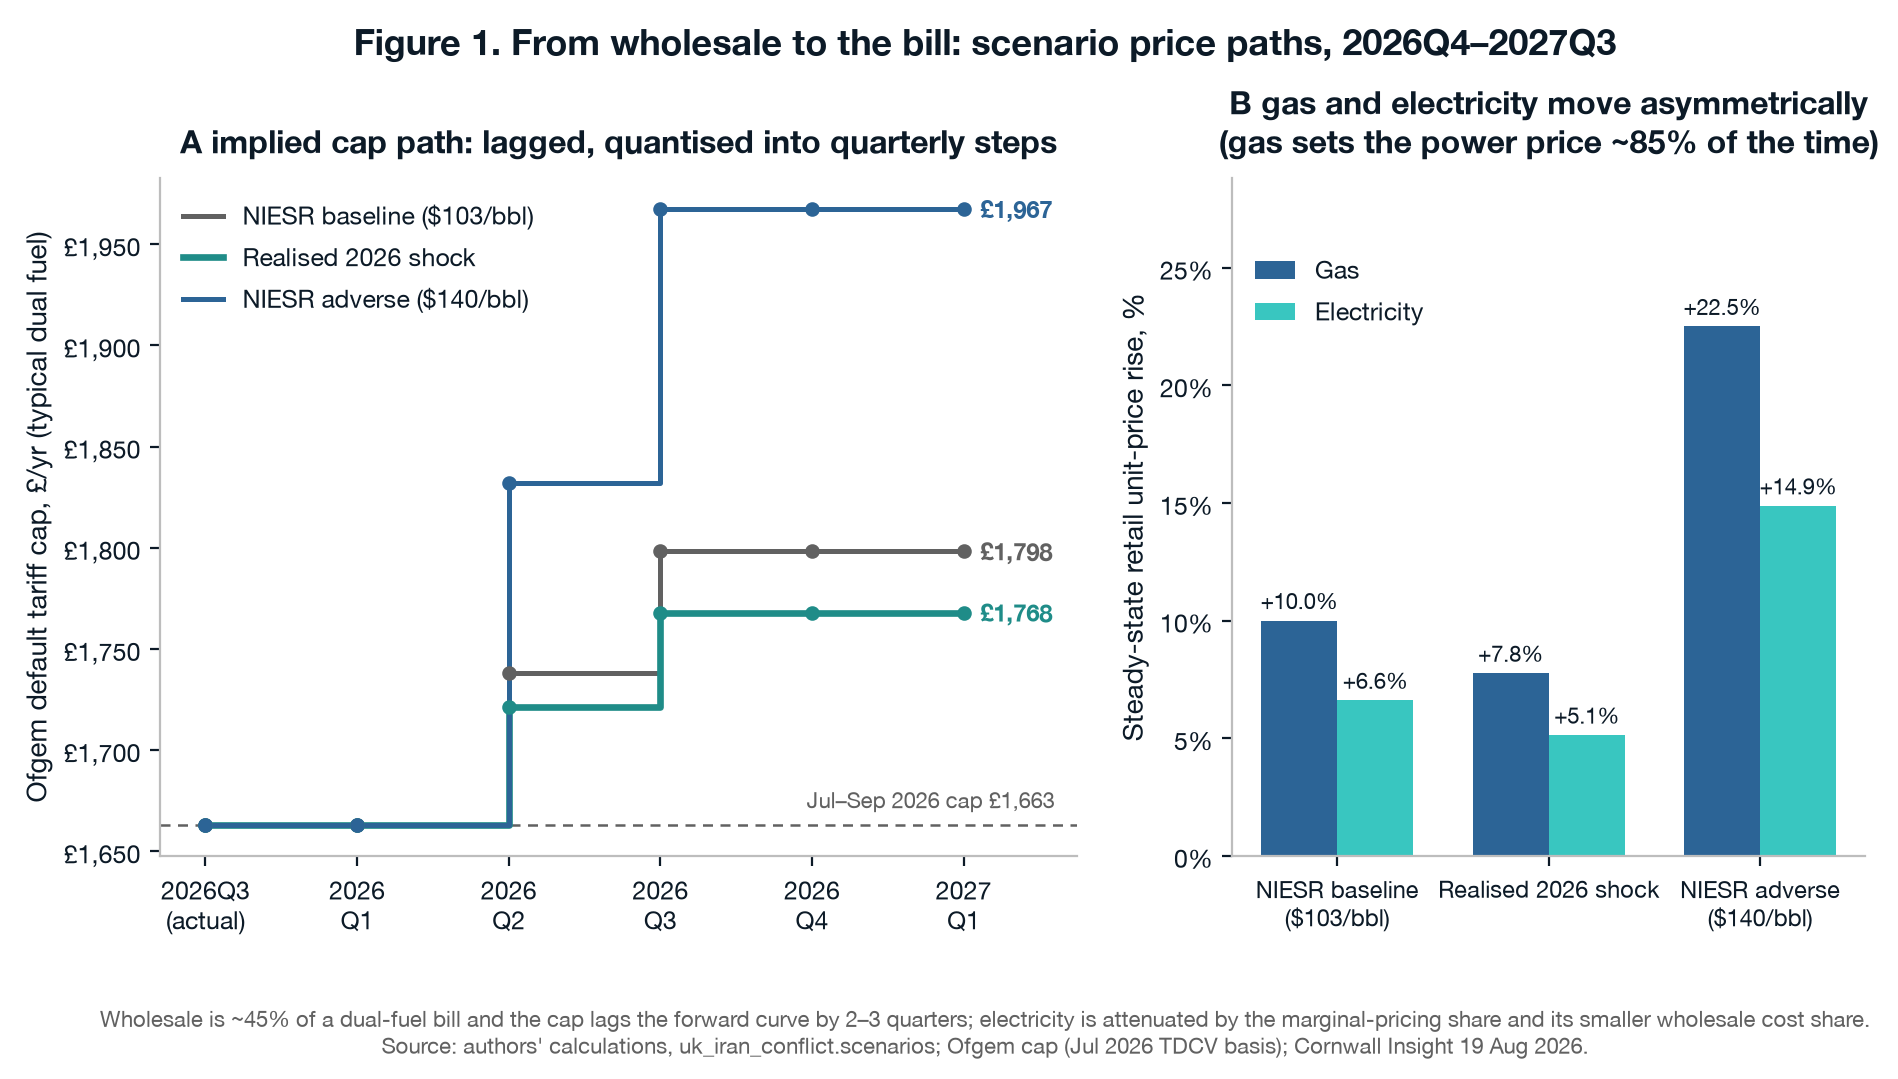
\includegraphics[width=.85\textwidth]{../results/figures/fig1_price_path.png}
\caption{Wholesale gas and oil paths and the implied Ofgem cap and pump-price paths, by scenario. The visible horizontal displacement between the wholesale series and the cap series is the two-to-three-quarter averaging lag; the vertical compression is the wholesale share of the bill.}
\label{fig:pricepath}
\end{figure}

Figure~\ref{fig:pricepath} makes the two transmission features visible at once: the lag between the wholesale move and the household bill, and the attenuation from the non-commodity components of the cap. It is also the figure that shows why peak-based bill-rise estimates in the policy literature exceed annualised ones.

\subsection{First-order incidence by decile}
\label{sec:results-decile}

Table~\ref{tab:decile} reports the annual cost increase by equivalised disposable income decile in pounds and as a share of income. The mean household loses \pounds \genCentralLossMean{}, or \genCentralLossPctIncome{} per cent of income. The two orderings diverge by construction of the underlying data rather than by assumption: in cash the loss rises across deciles, from \pounds \genDecileOneLossGbp{} in decile one to \pounds \genDecileTenLossGbp{} in decile ten, while as a share of income it falls, from \genDecileOneLossPct{} per cent to \genDecileTenLossPct{} per cent. The ratio of the bottom-decile to top-decile percentage loss is \genDecileRatioPct{}.

\begin{table}[htbp]
\centering
\caption{Annual household energy cost increase by equivalised disposable income decile, realised scenario: mean pound loss, loss as a share of equivalised disposable income, and the decomposition into gas, electricity and road fuel. Gross of any policy response.}
\label{tab:decile}
\begin{tabular}{lrrrrr}
\toprule
Decile & \pounds\ loss & \% of income & Gas & Electricity & Road fuel \\
\midrule
% populated from results/decile_incidence.csv
\multicolumn{6}{c}{\emph{[table body generated]}} \\
\bottomrule
\end{tabular}
\end{table}

\begin{figure}[htbp]
\centering
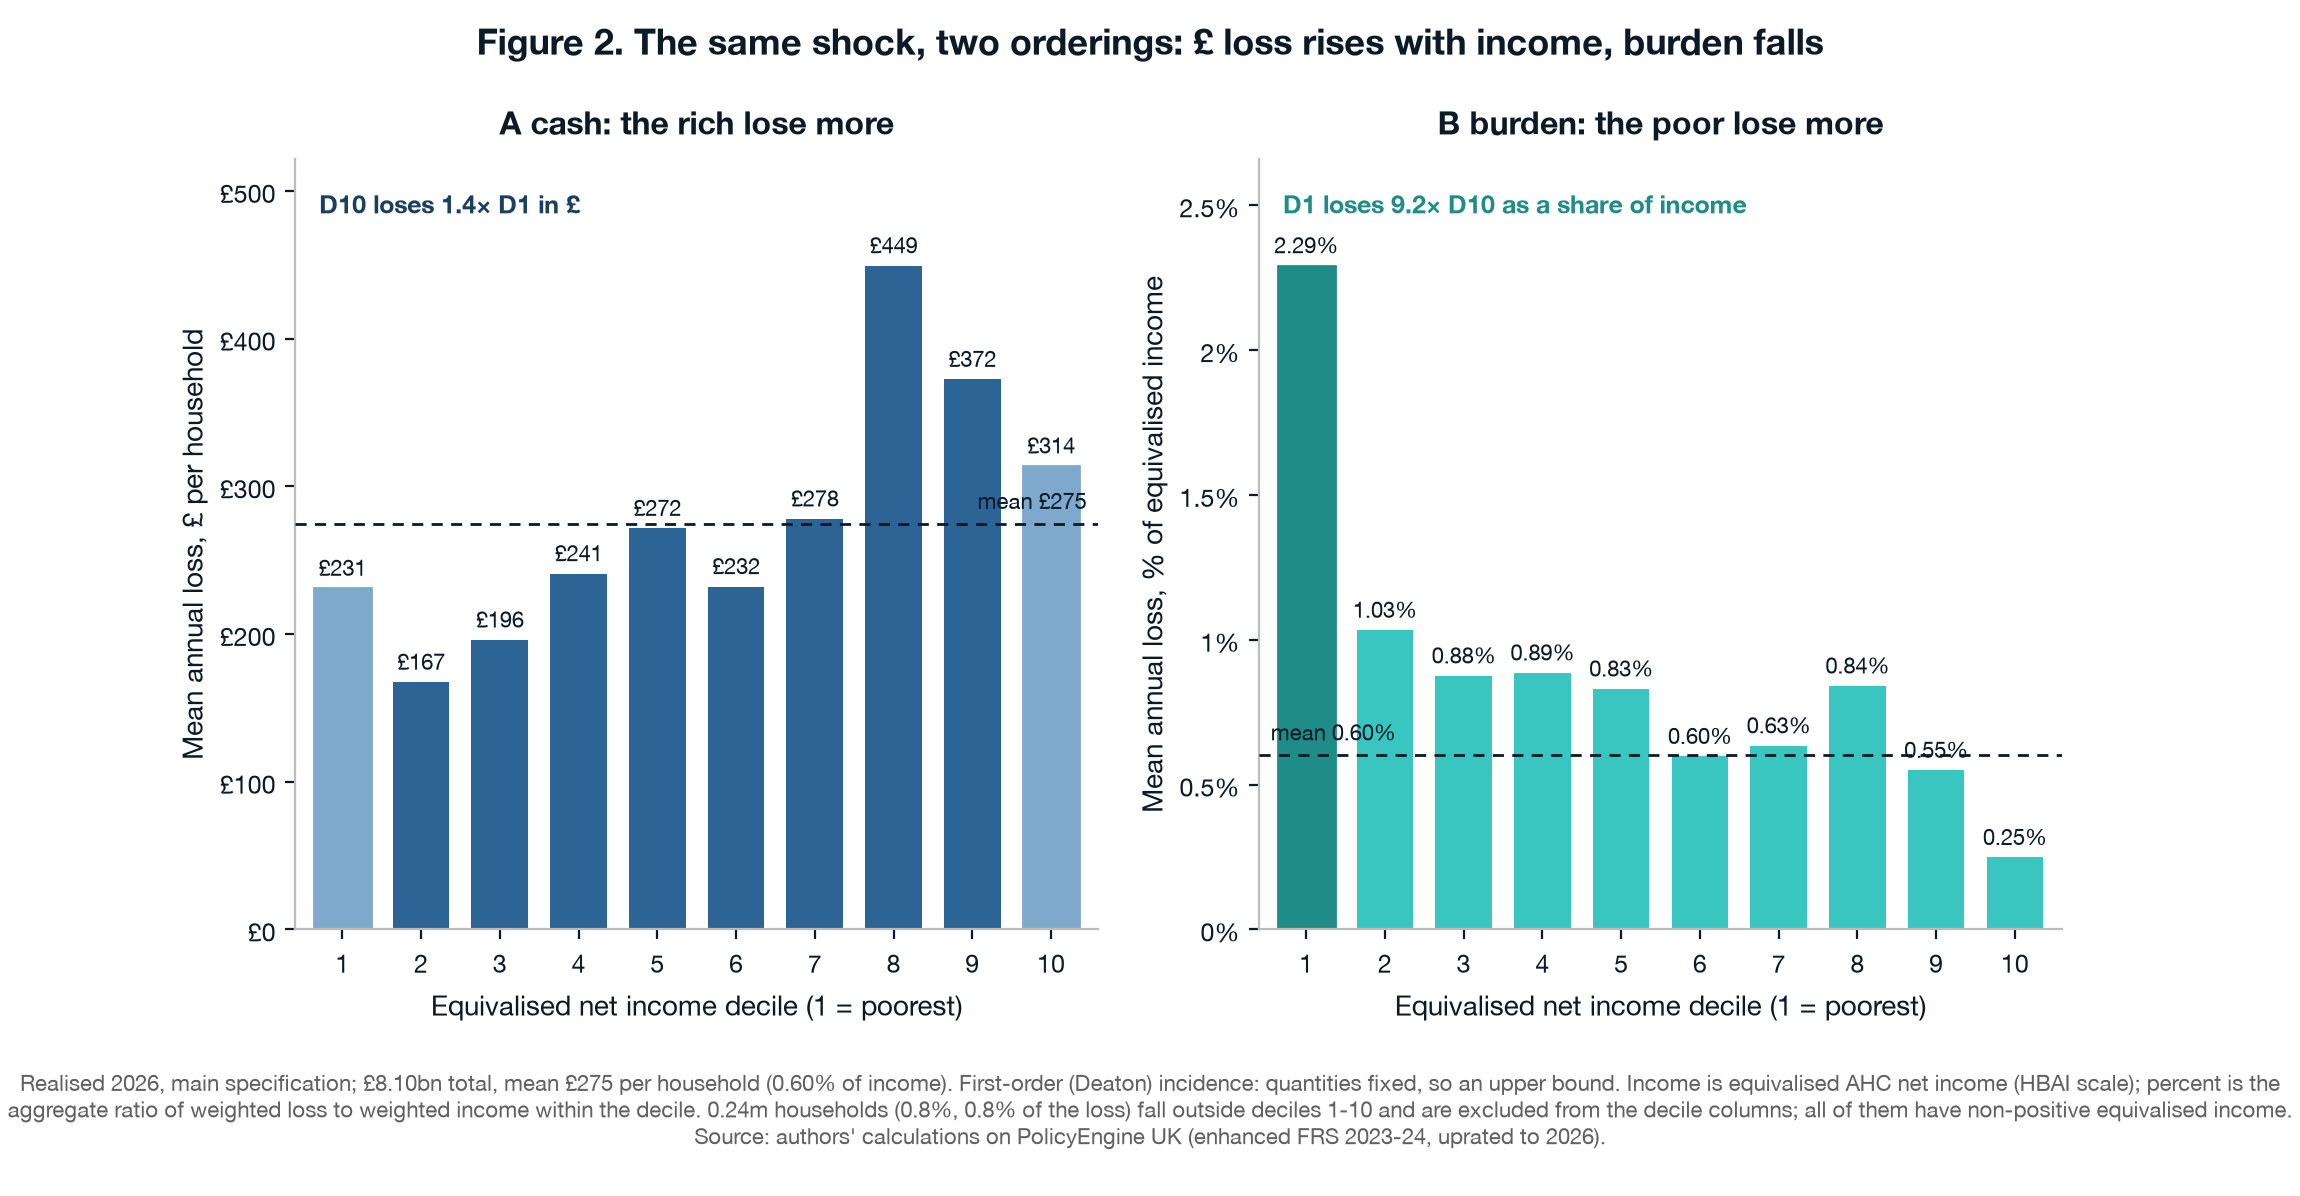
\includegraphics[width=.85\textwidth]{../results/figures/fig2_decile_dual.png}
\caption{Energy cost increase by income decile on two metrics: bars give the mean loss in pounds (left axis), the line gives the loss as a share of equivalised disposable income (right axis). The crossing of the two series is the paper's organising fact.}
\label{fig:deciledual}
\end{figure}

\begin{figure}[htbp]
\centering
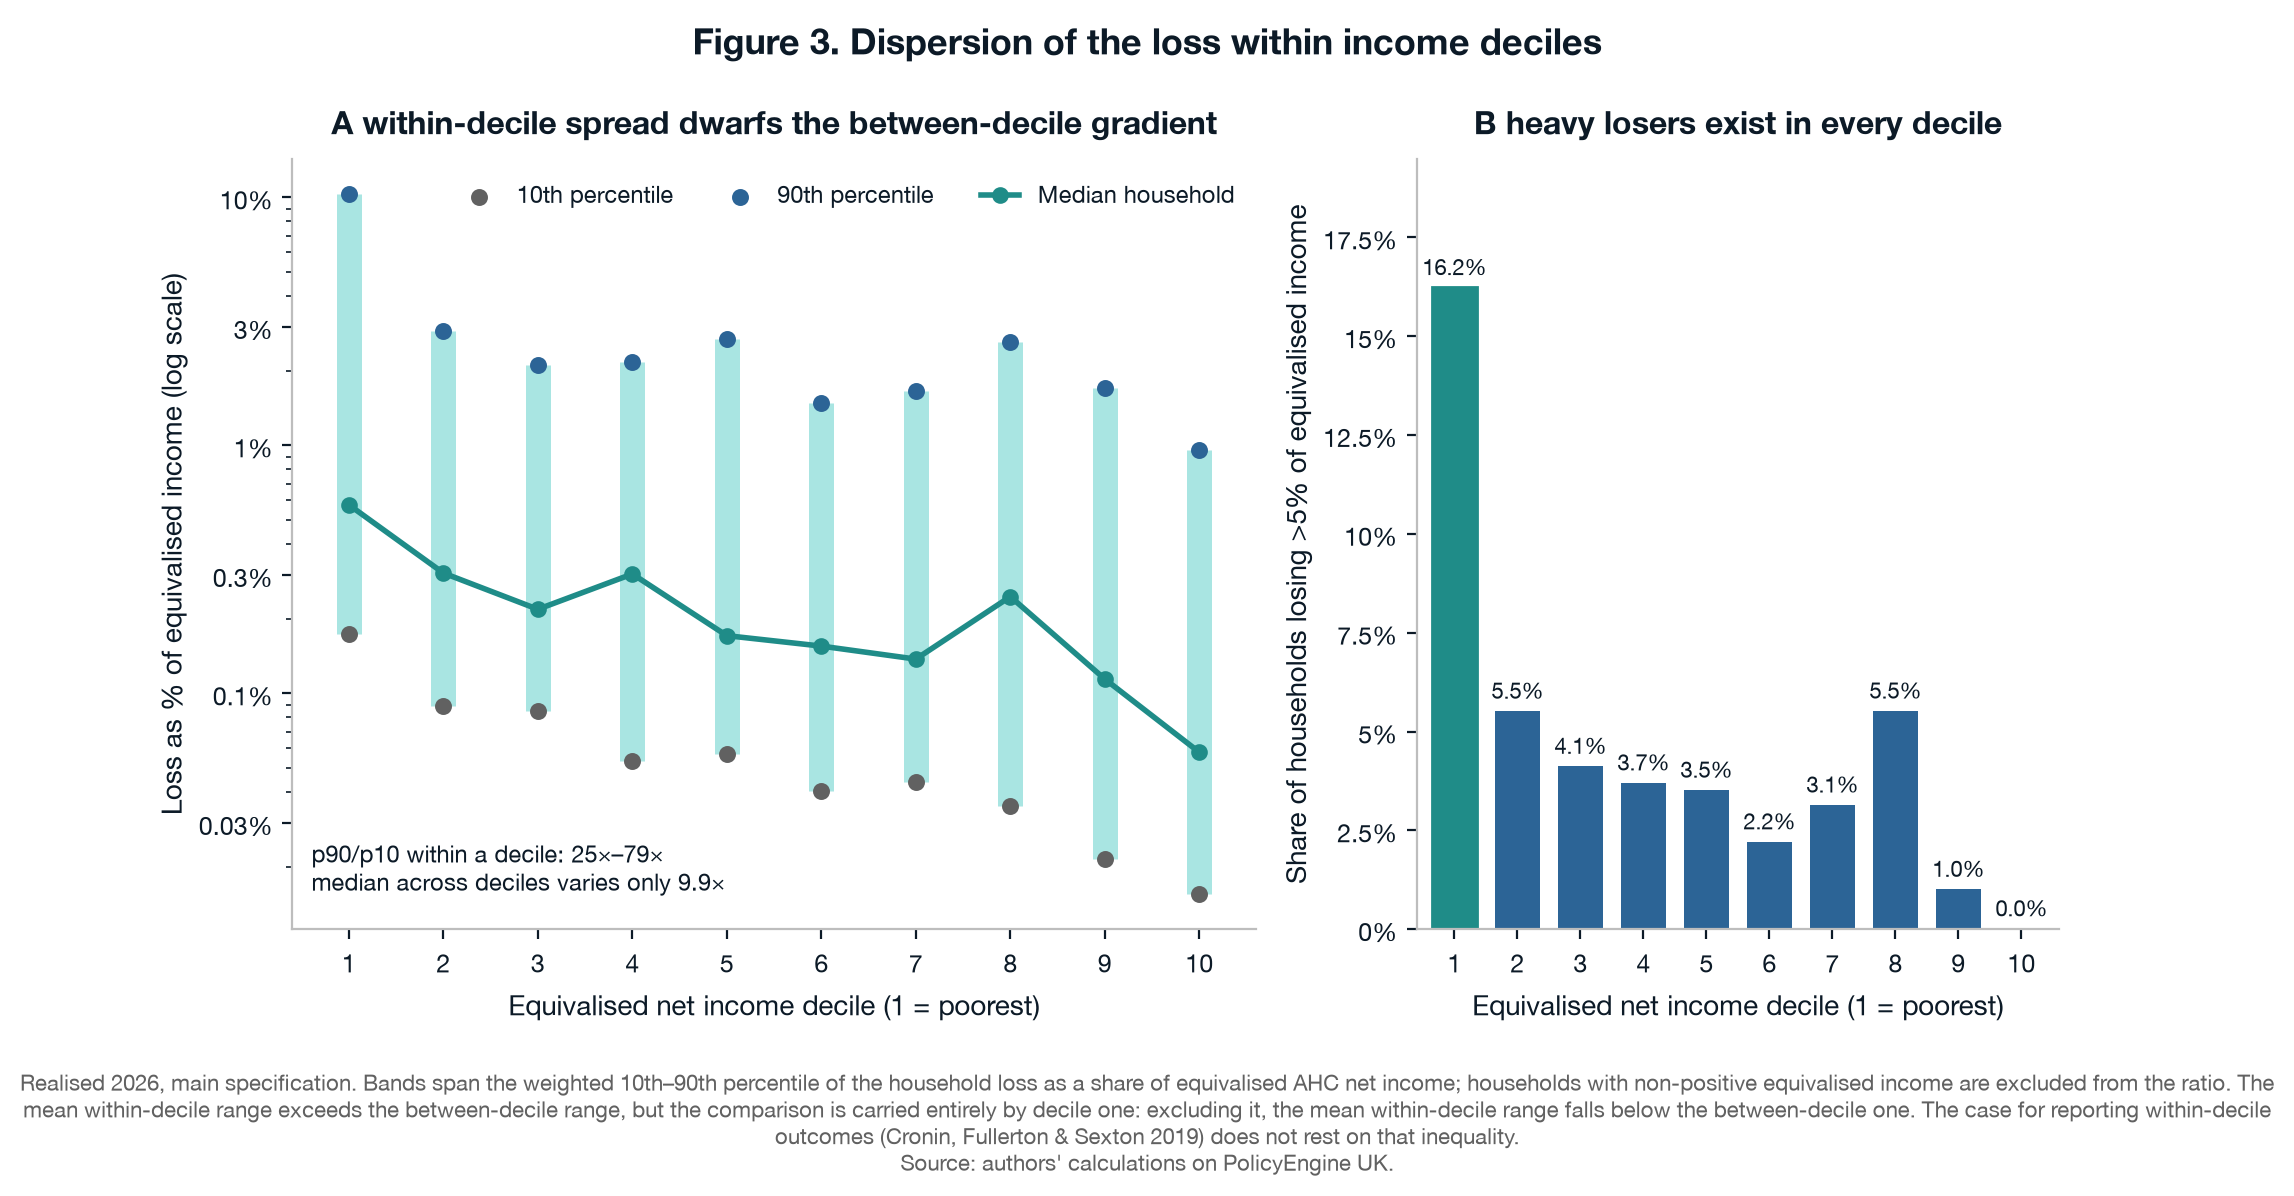
\includegraphics[width=.85\textwidth]{../results/figures/fig3_within_decile.png}
\caption{Within-decile dispersion of the percentage loss: box plots by decile with whiskers at the 10th and 90th percentiles. Shows how far horizontal dispersion inside each decile exceeds the vertical gradient across deciles.}
\label{fig:withindecile}
\end{figure}

Figure~\ref{fig:withindecile} is the within-decile counterpart. The interdecile range of the mean percentage loss is \genBetweenDecileRangePct{} percentage points, while the mean within-decile interdecile range is \genWithinDecileRangePct{} percentage points --- the quantitative form of the \citet{cronin2019} point, and the reason the uncompensated-loser metric in Section~\ref{sec:results-policy} does work that decile averages cannot.

\subsection{Fuel-mix and heating-type heterogeneity}
\label{sec:results-heterogeneity}

Table~\ref{tab:heating} breaks losses down by primary heating fuel and by on- versus off-gas-grid status. Because the shock is applied asymmetrically to gas and electricity, the ranking of household types is a direct consequence of the Step 1 calibration and not of the microdata alone: gas-heated households absorb the larger unit-rate move, while electrically heated and off-grid households face a smaller proportional move from a higher baseline unit cost. Off-gas-grid households lose \pounds \genOffGridLossGbp{} on average against \pounds \genOnGridLossGbp{} on grid.

\begin{table}[htbp]
\centering
\caption{Losses by primary heating fuel, gas-grid connection, tenure and household composition, realised scenario. Reported in pounds and as a share of income, with the population share of each group.}
\label{tab:heating}
\begin{tabular}{lrrr}
\toprule
Group & Population share & \pounds\ loss & \% of income \\
\midrule
% populated from results/heterogeneity.csv
\multicolumn{4}{c}{\emph{[table body generated]}} \\
\bottomrule
\end{tabular}
\end{table}

\subsection{Incidence by parliamentary constituency}
\label{sec:results-constituency}

Figure~\ref{fig:maps} is the paper's headline result: the same shock mapped across all 650 Westminster constituencies on the two metrics side by side. The left panel shades each seat by mean loss as a share of income; the right panel shades the same seats by mean loss in pounds. The two maps are close to negatives of one another. The Spearman rank correlation between the two constituency rankings is \genConstituencyRankCorr{}, and of the fifty seats worst affected in percentage terms only \genTailOverlapCount{} also appear among the fifty worst affected in pounds.

\begin{figure}[htbp]
\centering
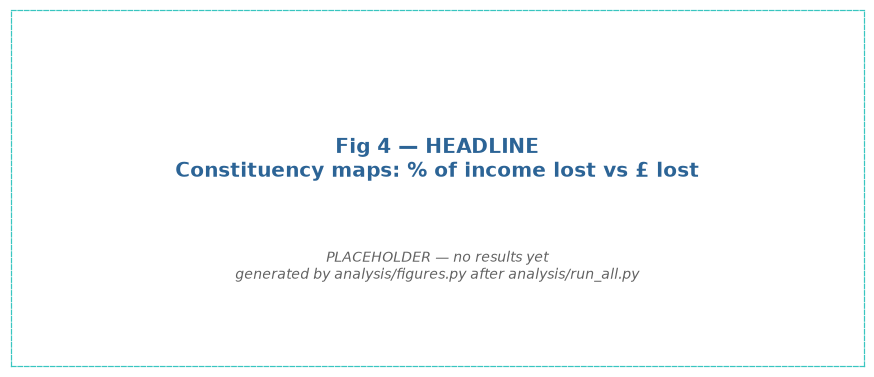
\includegraphics[width=\textwidth]{../results/figures/fig4_constituency_maps.png}
\caption{Energy cost increase by Westminster parliamentary constituency, realised scenario. Left: mean loss as a share of equivalised disposable income. Right: mean loss in pounds per year. Same shock, same households, same colour scale quantiles --- opposite geographies. Constituency estimates rest on re-optimised synthetic weights (Section~\ref{sec:limitations}); rankings are more reliable than levels.}
\label{fig:maps}
\end{figure}

\begin{figure}[htbp]
\centering
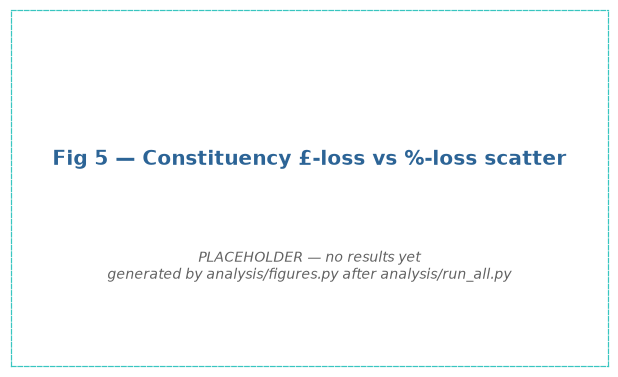
\includegraphics[width=.75\textwidth]{../results/figures/fig5_constituency_scatter.png}
\caption{Constituency-level scatter of pound loss against percentage-of-income loss, with seats in either tail labelled and marker size proportional to the seat's share of households on means-tested benefits. The scatter quantifies what the paired maps show qualitatively.}
\label{fig:constituencyscatter}
\end{figure}

\begin{table}[htbp]
\centering
\caption{The twenty constituencies worst affected on each metric, side by side, with each seat's rank on the other metric. Illustrates directly that a policy calibrated to one ranking misses the other.}
\label{tab:worstseats}
\begin{tabular}{lrrlrr}
\toprule
\multicolumn{3}{c}{Worst by \% of income} & \multicolumn{3}{c}{Worst by \pounds} \\
\cmidrule(lr){1-3}\cmidrule(lr){4-6}
Constituency & \% & \pounds\ rank & Constituency & \pounds & \% rank \\
\midrule
% populated from results/constituency_incidence.csv
\multicolumn{6}{c}{\emph{[table body generated]}} \\
\bottomrule
\end{tabular}
\end{table}

\subsection{Scenario comparison}
\label{sec:results-scenario}

Table~\ref{tab:scenario} sets the three scenarios against one another on the headline aggregates: total additional household energy spending, the mean loss, the bottom-decile percentage loss, and the number of households pushed below the fuel-poverty and relative-poverty thresholds. Aggregate additional household energy and fuel spending is \pounds \genAggSpendRealisedBn{} billion in the realised scenario against \pounds \genAggSpendAdverseBn{} billion in the adverse one.

\begin{table}[htbp]
\centering
\caption{Headline aggregates under the baseline, realised and adverse scenarios. Static, use-side only, zero-elasticity; see Section~\ref{sec:limitations}.}
\label{tab:scenario}
\begin{tabular}{lrrr}
\toprule
& Baseline & Realised & Adverse \\
\midrule
% populated from results/scenario_summary.csv
\multicolumn{4}{c}{\emph{[table body generated]}} \\
\bottomrule
\end{tabular}
\end{table}

\subsection{Scoring the policy responses}
\label{sec:results-policy}

Table~\ref{tab:scorecard} scores the five responses of Section~\ref{sec:step4} on the three metrics. The means-tested social tariff delivers \genSocialTariffShareBottomThree{} per cent of its spend to deciles one to three at a cost of \pounds \genSocialTariffCostBn{} billion, but leaves \genSocialTariffUncompensatedShare{} per cent of losing households uncompensated. The JRF universal discounted block costs \pounds \genJrfCostBn{} billion and leaves \genJrfUncompensatedShare{} per cent uncompensated, delivering \genJrfShareBottomThree{} per cent of spend to deciles one to three. The Warm Home Discount expansion costs \pounds \genWhdCostBn{} billion; the VAT cut on domestic fuel costs \pounds \genVatCutCostBn{} billion and delivers \genVatCutShareBottomThree{} per cent to the bottom three deciles; the flat rebate costs \pounds \genRebateCostBn{} billion. Cost per pound of bottom-decile gain runs from \pounds \genBestCostPerPound{} to \pounds \genWorstCostPerPound{} across the five.

\begin{table}[htbp]
\centering
\caption{Policy scorecard: exchequer cost, cost per pound of bottom-decile gain, share of spend reaching deciles one to three, and share of losing households left uncompensated, for each of the five responses, evaluated against the realised scenario.}
\label{tab:scorecard}
\begin{tabular}{lrrrr}
\toprule
Reform & Cost (\pounds bn) & \pounds\ per \pounds\ D1 gain & \% to D1--D3 & \% losers uncompensated \\
\midrule
% populated from results/policy_scorecard.csv
\multicolumn{5}{c}{\emph{[table body generated]}} \\
\bottomrule
\end{tabular}
\end{table}

\begin{figure}[htbp]
\centering
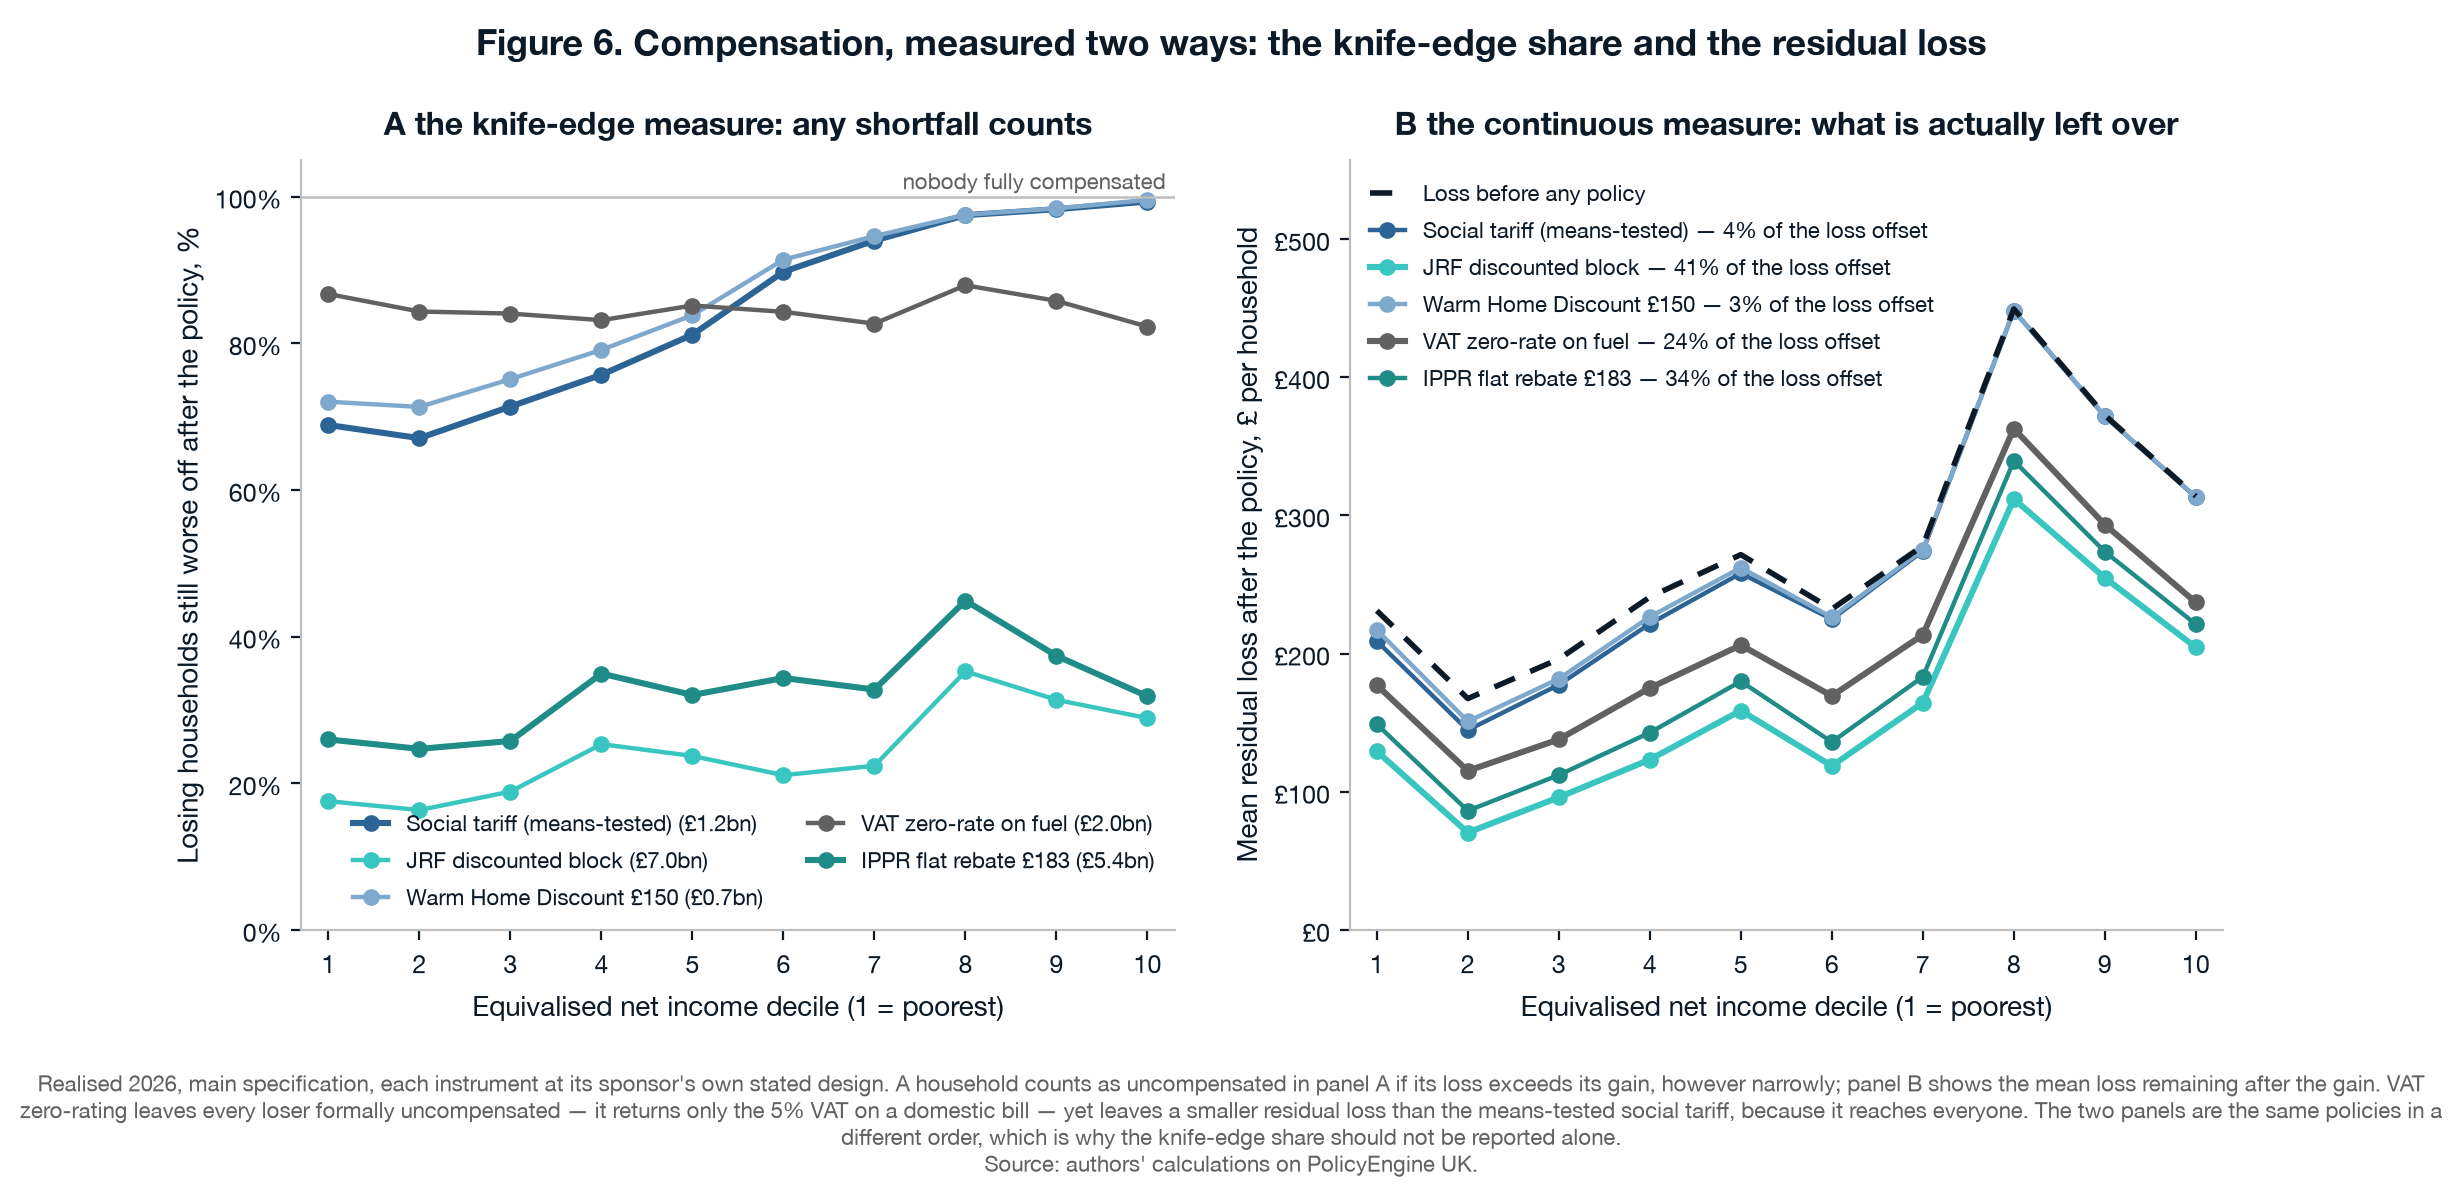
\includegraphics[width=\textwidth]{../results/figures/fig6_uncompensated.png}
\caption{Share of losing households left uncompensated within each income decile, by policy. The between-decile targeting metrics rank the policies one way; this within-decile metric ranks them differently, which is the substance of Section~\ref{sec:policy}.}
\label{fig:uncompensated}
\end{figure}

\begin{figure}[htbp]
\centering
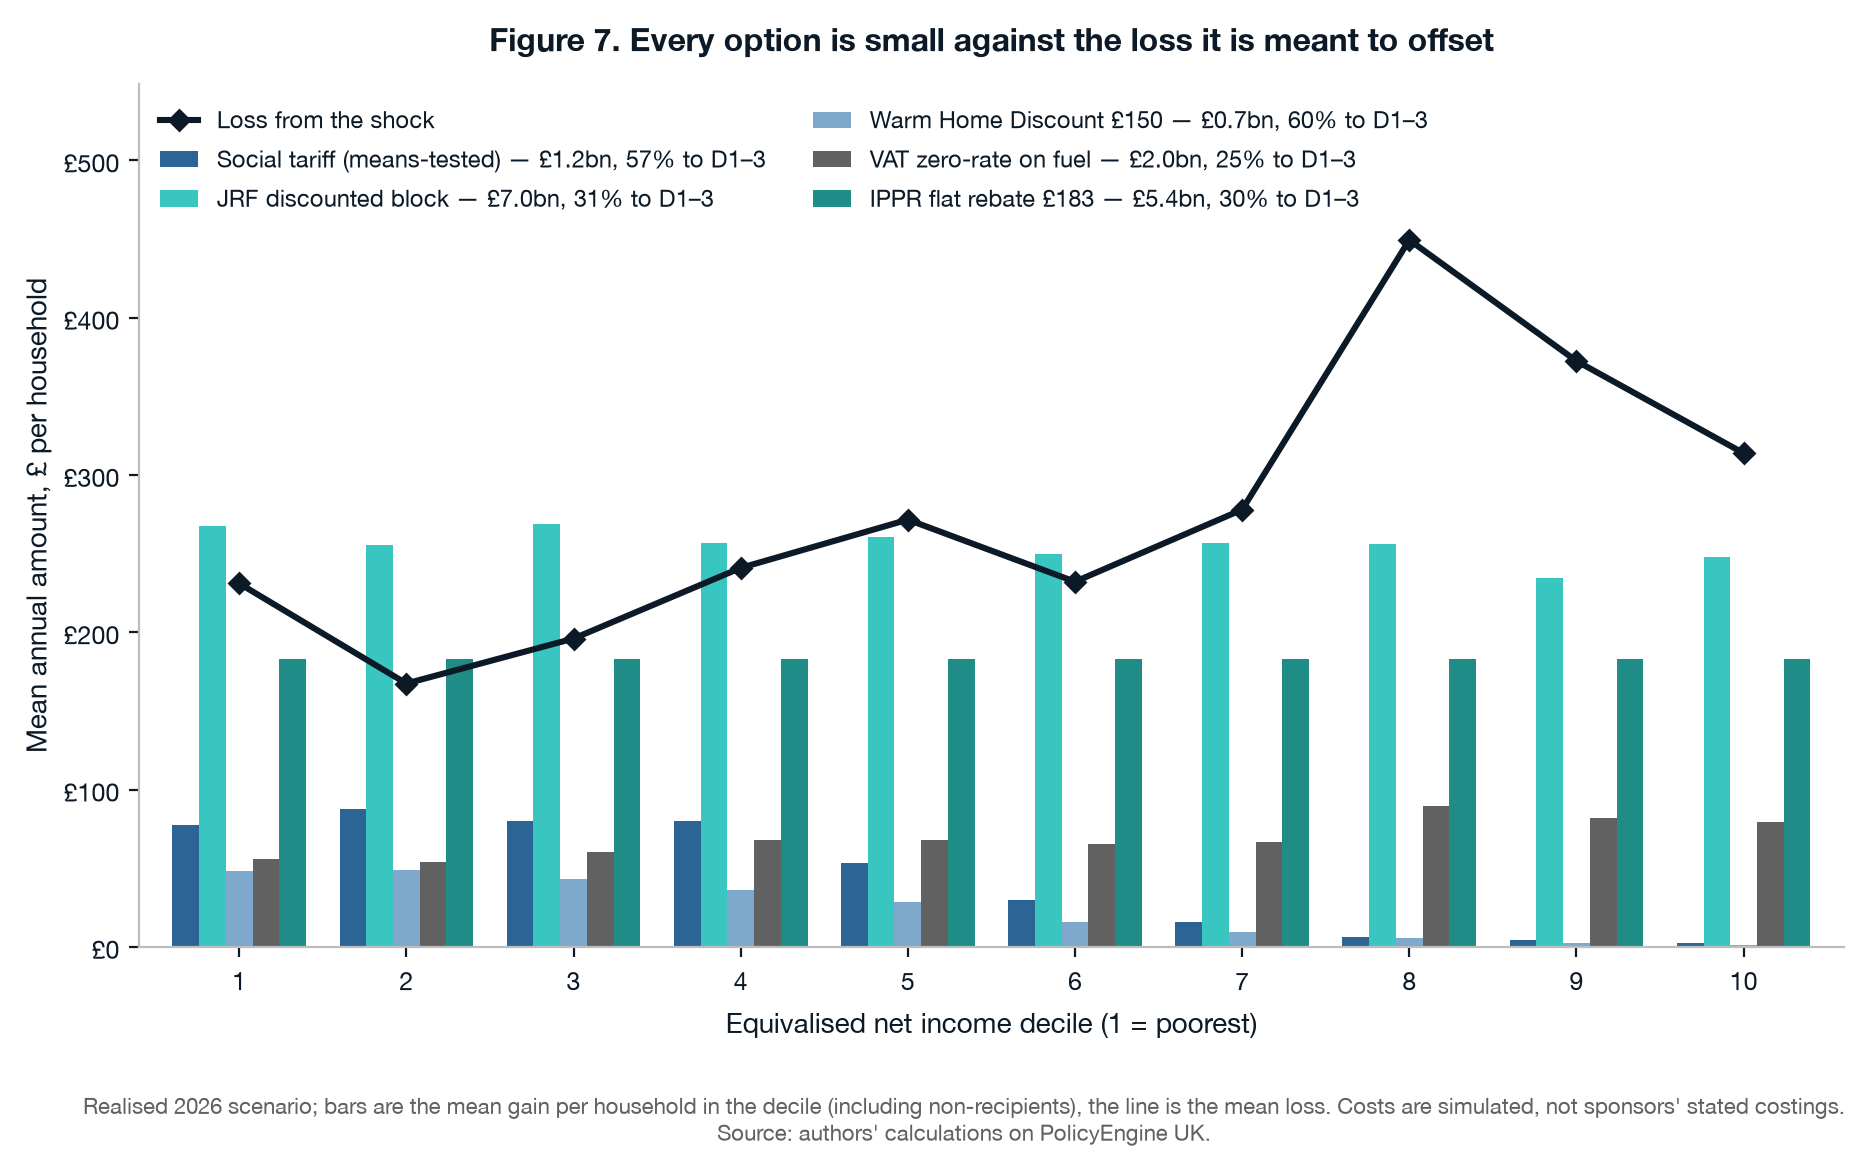
\includegraphics[width=.85\textwidth]{../results/figures/fig7_policy_deciles.png}
\caption{Net change in household disposable income by decile under each policy, shock included, as a share of baseline income. Shows which policies fully offset the shock at the bottom and where each leaves a residual loss.}
\label{fig:policydeciles}
\end{figure}

\begin{figure}[htbp]
\centering
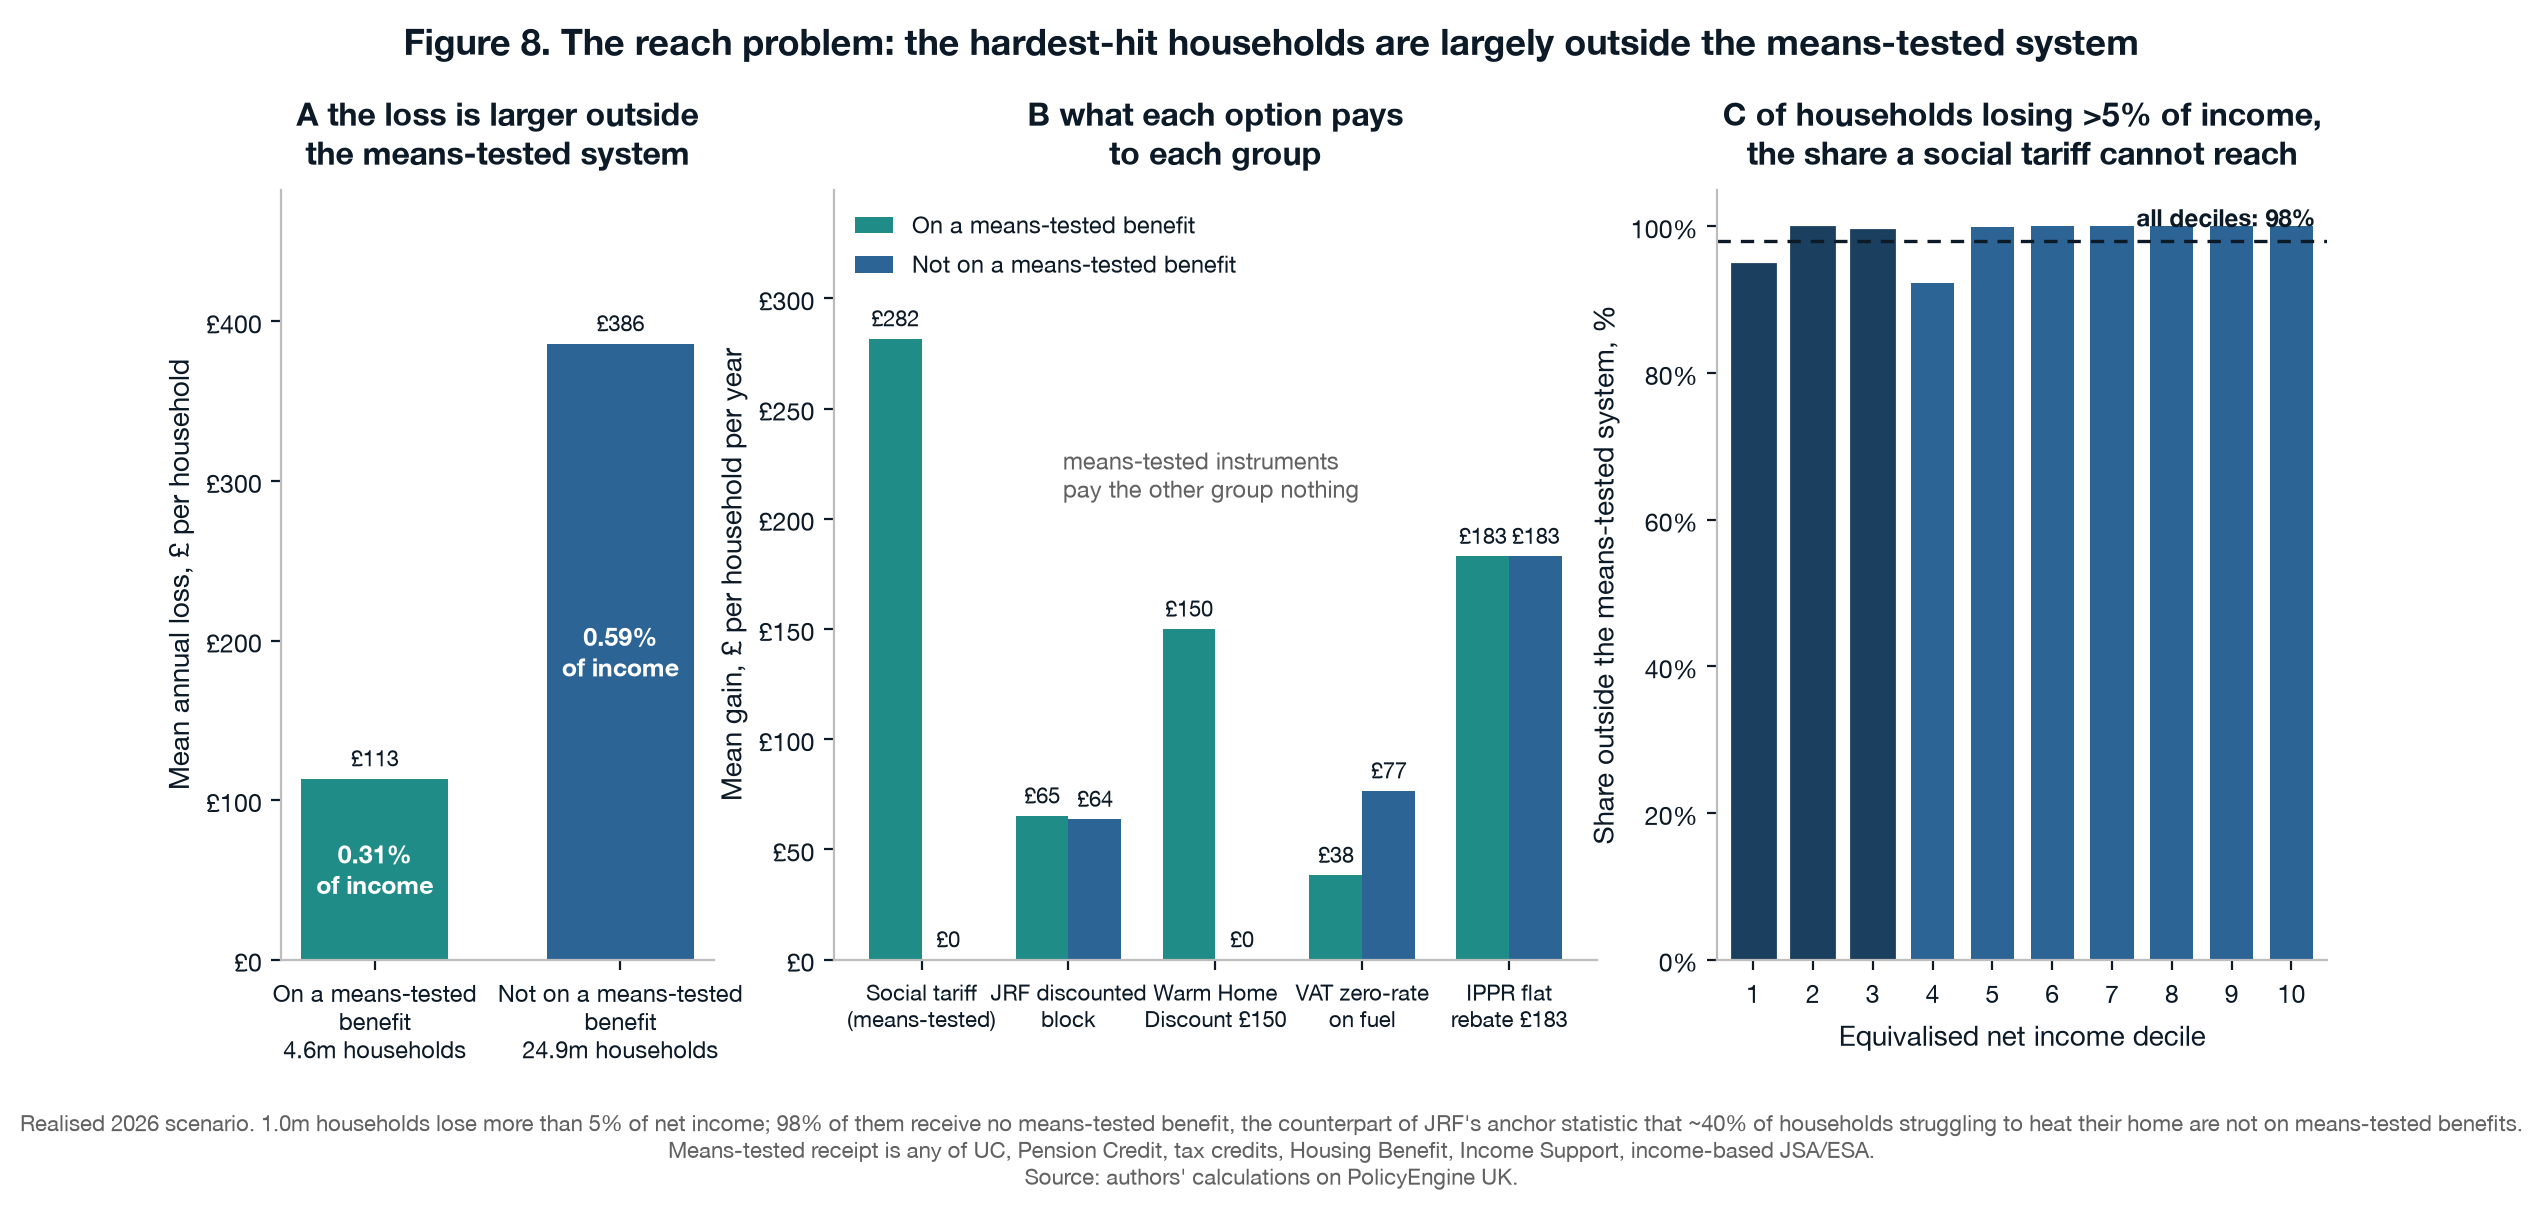
\includegraphics[width=.85\textwidth]{../results/figures/fig8_benefit_status.png}
\caption{Compensation rates split by receipt of means-tested benefits. The quantitative form of the \genNonMeansTestedStruggling{} per cent statistic: the share of struggling households outside the means-tested system, and what each policy delivers to them.}
\label{fig:benefitstatus}
\end{figure}

\section{The Autumn Budget 2026 choice}
\label{sec:policy}

The results in Section~\ref{sec:results} bear directly on a decision that has not yet been taken. The Chancellor has ruled out universal support of the 2022 kind and signalled income-based help --- in practice, a social tariff --- while the Joseph Rowntree Foundation and the TUC have pressed for a universal discounted block costing around \pounds 5 billion. This section sets out what the two designs do differently, why the disagreement is not really about generosity, and what the model says about the third option nobody is arguing for.

\subsection{Two designs, one disagreement}

A \emph{means-tested social tariff} conditions a discounted unit rate on receipt of a qualifying benefit. Its appeal is arithmetic: every pound of spend goes to a household that has already passed a means test, so on the two conventional targeting metrics --- share of spend reaching the bottom three deciles, and cost per pound of bottom-decile gain --- it will dominate any untargeted alternative, and Table~\ref{tab:scorecard} confirms it does.

The \emph{universal discounted block} does something structurally different. It prices the first half of typical consumption at a discounted rate and everything above it at the full rate, with a per-child allowance recognising that household need scales with size. Because the discount applies to a fixed quantity rather than to all consumption, its cash value is roughly flat across the distribution while high-consumption households --- disproportionately affluent, per \citet{fetzer2024} --- pay the full marginal rate on the bulk of their usage. It is therefore neither a universal price subsidy of the Energy Price Guarantee type, which cost around \pounds 23 billion and was regressive in cash terms precisely because it subsidised every unit, nor a transfer. JRF costs it at roughly \pounds 5 billion and argues it fully offsets the modelled cost increase for deciles one to three. They also argue, on operational rather than distributional grounds, that a social tariff cannot be built in time for winter 2026: there is no register of eligible households that is both current and complete, and constructing one is a multi-year data-sharing project.

The disagreement is not about how much to spend. It is about a coverage gap.

\subsection{The crux: the households outside the means test}

Approximately 40 per cent of households struggling to heat their homes are not on means-tested benefits. This single statistic is the anchor of every submission to the Budget, and it is what our uncompensated-loser metric measures directly. A means test that is perfectly accurate on the population it covers still leaves the entire uncovered population at zero compensation, and that population is not a random sample of the non-poor: it is concentrated among low-income households above the benefit taper, households with savings above the capital limit, pensioners on modest occupational incomes, the self-employed with volatile earnings, and non-claimants --- take-up of means-tested support is materially below entitlement and is lowest among precisely the groups whose energy exposure is highest.

The reform to the Warm Home Discount that took effect for the 2026--27 scheme year --- the qualifying date was 23 August 2026, the property-cost test is scrapped, the \pounds 150 payment is now automatic in England and Wales, and around 2.7 million additional households are brought in --- narrows this gap but does not close it, because eligibility still runs through benefit receipt. The expansion moves the uncompensated share in the right direction; it does not change the structure that generates it.

Figure~\ref{fig:uncompensated} is therefore the policy-relevant figure rather than Table~\ref{tab:scorecard}. Read on between-decile targeting, the social tariff wins. Read on within-decile coverage, it does not, because the losers it misses are systematically the ones no observable identifies. This is \citet{sallee2019}'s result in applied form: when transfers must condition on observables, compensating every loser is not merely expensive but infeasible, and the residual is not noise. \citet{cronin2019} and \citet{douenne2020} establish the same point from the incidence side --- horizontal redistribution within income groups routinely exceeds vertical redistribution between them --- which means a scorecard that reports only decile means is measuring the smaller of the two effects.

\subsection{Against the ``never subsidise prices'' consensus}

The grey-literature consensus after 2022 is unambiguous: compensate incomes, not prices. \citet{ari2022} is the standard reference, and the Bruegel fiscal tracker's finding that only around a third of European energy support was targeted is the standard evidence. The reasoning is familiar --- a price subsidy distorts the marginal incentive to conserve, its cost scales with consumption and therefore with affluence, and it blunts the very price signal that is supposed to induce adjustment.

The peer-reviewed frontier does not agree. \citet{levell2025}, the closest thing to a definitive treatment of the 2022--23 UK episode, estimate a mean welfare loss of about 6 per cent of income absent policy, find that the actual UK package reduced both the mean and the dispersion of losses at an efficiency cost of about 12 per cent of its revenue cost, and --- the result that matters here --- show that the constrained-optimal policy includes a \emph{strictly positive price subsidy}. The subsidy shrinks as the transfer instrument is allowed to condition on more information, in particular on income \emph{and past energy usage} jointly, but it does not go to zero. The reason is exactly the coverage gap of the previous subsection: a price subsidy reaches households that no observable-based transfer can identify, and when the untargeted population is large, the insurance value of that reach outweighs the deadweight loss from the distorted margin.

This reframes the Budget choice. The question is not whether to subsidise prices --- the answer is that a positive subsidy belongs in the optimum --- but how large the price component should be given the transfer instruments actually available. The universal discounted block is a coherent answer to that question and not merely a political compromise: it is a price subsidy on an inframarginal quantity, which preserves the marginal price signal above the block while delivering the reach that a means test cannot. That is close to the two-tier tariff \citet{fetzer2024} propose on entirely separate evidence, and close to the structure \citet{levell2025} recover as optimal when the transfer instrument can condition on past usage --- which, as it happens, the block design does implicitly by defining the block relative to typical consumption.

\subsection{Financing}

The financing side is scored separately, because netting it into the household distribution would conflate two distinct incidence questions.

IPPR's proposal is to claw back windfalls accruing to regulated network companies --- whose allowed returns were set against a very different cost of capital and whose revenues are indexed --- and return the proceeds as a flat household rebate of around \pounds 183. As a distributional object a flat rebate is progressive in percentage terms and reaches every household regardless of benefit status, so it scores well on the coverage metric and poorly on the targeting metrics; it is the mirror image of the social tariff, and Table~\ref{tab:scorecard} shows the two failing on opposite metrics. Its distinctive feature is that its financing is close to a pure rent tax and therefore carries little efficiency cost, which is not true of the alternatives.

The other financing routes on the table are the successor arrangements to the Energy Profits Levy on oil and gas production, and an increase in the Electricity Generator Levy from 45 to 55 per cent. Both are windfall instruments whose yield is mechanically correlated with the shock being compensated, which is an attractive property: the fiscal cost of support and the revenue that pays for it move together, so the package is closer to self-financing in the adverse scenario than in the baseline. Both also carry investment-margin costs that a static microsimulation cannot evaluate and that the source-side literature \citep{goulder2019} suggests are progressive in incidence --- reducing returns to capital falls on capital owners, who are concentrated at the top --- so excluding them from the household results understates the progressivity of the financed package as a whole. I report the household side of each policy and the aggregate cost, and note the direction of the omitted source-side effect rather than attempting to quantify it.

\section{Discussion}
\label{sec:discussion}

Four findings, and each is bounded by something the design cannot recover. Motor fuel is the largest single channel at \genMotorFuelShareOfLoss{} per cent of the aggregate loss, but between \genSpecFuelShareMinPct{} and \genSpecFuelShareMaxPct{} per cent across specifications and wider still across the gas-peak profiles the pre-war solve consumes; what holds across that range is that a large part of the shock, never less than \genSpecFuelShareMinPct{} per cent, arrives through a channel every instrument in the Budget debate leaves untouched. The cap formula can carry a macro scenario to a household price vector, but only against a counterfactual it does not supply: the pre-war level is solved, at \pounds \genCapBaselineLevel{}, and its fragility to the gas-peak profile --- \pounds \genGasProfileAggMinBn{} to \pounds \genGasProfileAggMaxBn{} billion, with \genGasProfileNonIdentifiedCount{} of \genGasProfileCellCount{} profiles admitting no solution --- is the paper's principal uncertainty. The burden falls in income in every specification while the cash loss does not, though the steepness is uncertain by more than a factor of two and every gradient here is ranked on before-housing-costs income and measured on after-housing-costs income (Section~\ref{sec:limitations}). And eligibility rather than generosity is the binding margin on an exchequer envelope, by a factor the means-tested fuel imputation does not pin down.

Two of those results deserve a note about what stabilises them. Measured on the domestic channel alone the decile gradient is \genDomesticOnlyDecileRatioPct{} to one in every one of the seven specifications and every cell of the scenario grid, so the variation in the all-channel figure is located in the fuel imputation rather than in the domestic leg. And the eligibility finding survives every admission rule scored, including a lottery: what the perfect-observability assumption buys is targeting, not offset. No constituency-level claim is made anywhere: the data release has no constituency weight matrix and a degenerate local-authority field, and no approximation is offered in place of one.

\subsection{The K\"anzig caveat}

The most serious objection is that this paper measures the wrong channel. \citet{kanzig2023} shows that poorer households lose from energy shocks disproportionately through employment and earnings rather than budget shares, with general-equilibrium and indirect effects accounting for roughly two-thirds of the household response, none of which a static use-side microsimulation captures. \citet{goulder2019} sharpen the point --- use-side effects regressive, omitted source-side effects progressive --- and \citet{ohlendorf2021}'s meta-analysis is the summary statement. It constrains the claims here in three ways.

\emph{Magnitude.} If the use-side channel is roughly a third of the total, the losses reported are a lower bound on total household incidence, and a bottom-decile loss of \genDecileOneLossPct{} per cent of income is the part attributable to the price of energy alone. A reader wanting a total should multiply, acknowledging that the multiplier is borrowed from a different country and identification strategy.

\emph{Ordering.} Känzig's mechanism operates through employment, which is more concentrated among lower-income households than energy budget shares are, so the omitted channel almost certainly reinforces the percentage regressivity --- but it may well \emph{reverse} the cash ordering, since employment losses in pounds are larger higher up the earnings distribution. A general-equilibrium version of this exercise would not rescale the cash profile; it would redraw it.

\emph{Policy inference.} The compensation metrics are internally consistent, so the ranking of policies is more robust than the levels, provided instruments are compared at a common envelope and on more than the knife-edge count. But a policy scored as fully compensating a household on its use-side loss is not thereby compensating that household, and no policy in the scorecard addresses the income channel at all.

There is a countervailing consideration. \citet{pallotti2024} find that euro-area heterogeneity in 2021--23 was driven mainly by nominal net asset positions rather than energy basket composition. If the same holds for the UK, both the use-side channel modelled here and Känzig's employment channel are second to a balance-sheet channel requiring an up-to-date wealth distribution; the model's wealth imputation rests on Wealth and Assets Survey round 7 (2018--20), so this paper cannot speak to it.

\subsection{Three gaps this paper makes visible}

\paragraph{(a) UK wholesale-to-retail pass-through in the price-cap era.} The coefficient $\phi_f$ and lag $\ell$ in equation~\eqref{eq:passthrough} are calibrated from the published structure of the cap rather than estimated, because there is no well-cited econometric estimate of pass-through for the UK under the default tariff cap. The pre-cap literature is not transferable: the cap replaced competitive-retail pricing with a formula, amended repeatedly since 2019, so the estimation problem is regime-switching on a short sample. The data exist --- Ofgem publishes cap decompositions, averaging windows and announcement dates, and forward curves are observable daily --- and identification comes from the announcement calendar itself, the cap being a deterministic function of forwards over a pre-announced window, so the residual is the object of interest for fixed-tariff and out-of-cap customers. This is the most tractable of the three gaps and would tighten every number here.

\paragraph{(b) Energy arrears as an outcome variable.} The outcome here is a cost increase; the observable manifestation of the 2026 shock is debt, with JRF reporting around 1.5 million families in arrears and 3.8 million households owing roughly \pounds 7.5 billion. Arrears depend on liquidity, credit access, supplier forbearance and the prepayment split, so modelling them needs an intertemporal margin the model lacks, and modelling the policy response needs debt-related allowances --- which sit inside the cap, so that arrears feed back into everybody's unit rate. That within-consumer cross-subsidy has not been quantified for the UK, and it would change the policy ranking, since a social tariff that prevents arrears has a fiscal return the scorecard does not credit.

\paragraph{(c) Off-gas-grid and rural horizontal losers.} \citet{douenne2020} shows for France that flat recycling is progressive on average while creating large horizontal losers among rural and off-grid poor households. There is no UK counterpart and this paper does not supply one: the microdata contain no primary-heating-fuel indicator and no gas-grid flag, so losses cannot be split on gas-grid status at all, and no imputed stand-in is offered. The gap is live --- roughly four million UK properties are off the gas grid, heating oil and LPG sit outside the price cap, and these households were repeatedly omitted from 2022 support schemes --- and the finding that motor fuel carries a large part of the loss makes it sharper, since rural transport dependence and off-grid heating coincide in the same households.

\subsection{Where this leaves the macro-to-micro link}

The Seventh Carbon Budget established ``macro model plus distributional annex'' as the expected format for UK official analysis, but the annex is typically produced by a separate method on separate data, so the macro and micro numbers are not mutually consistent. What this paper does is small but structural: it fixes a single explicit transmission mechanism as the bridge --- the cap formula for domestic energy, and for road fuel a pass-through coefficient fitted to observed pump outturns --- so that the household results are a deterministic function of the macro scenario and can be regenerated when the scenario changes. The bridge is one-way, covers only the price channel, and sits alongside the tax-benefit model rather than inside it, because the model has no price channel to host it. Moving it inside, extending it to the income channel, and closing the loop so that the household response feeds back into aggregate demand is the natural continuation, and gap (a) is its prerequisite.


\clearpage
\bibliography{references}
\clearpage
\appendix
\section{Sensitivity, robustness and reproduction}
\label{sec:appendix}

Several sweeps and specification variants are reported here, each re-running the full pipeline on the realised 2026 central scenario against the same baseline. They are presented in order of how much they move the answer, and that ordering is the appendix's main message. It has been inverted by this revision, and the inversion matters enough to state at the top.

Earlier versions of this appendix instructed the reader to direct scepticism at the demand-elasticity assumption and nowhere else. That instruction was an artefact of measuring demand response as a change in \emph{expenditure} rather than as a change in \emph{welfare}: a household that stops heating its home spends less, and counting that as a saving is exactly the ``heat or eat'' fallacy this appendix criticises elsewhere. Measured as a money-metric welfare loss --- bounded above by the Laspeyres term and below by the Paasche term --- demand response removes at most \genWelfareShavedHighEpsPct{} per cent of the loss at the most elastic point of the grid, not the \genSpendShavedHighEpsPct{} per cent the expenditure measure suggested.

\textbf{The honest uncertainty ranking is therefore: the motor-fuel and domestic-energy imputations first, the accounting basis --- phase-in against steady state, equivalised against unequivalised --- second, the pass-through and damping calibration third, and the demand elasticity a distant fourth.} A reader deciding where to direct scepticism should direct it at the first three.

No constituency-level robustness statistic appears in this appendix. The data release carries no constituency weight matrix, so seat-level rank correlations are not computable and none has been substituted (Section~\ref{sec:step3}).

\subsection{Demand response: smaller than it looked}
\label{app:elasticity}

The main specification is zero-elasticity by construction: equation~\eqref{eq:firstorder} evaluates the price change at pre-shock quantities, which is the \citet{deaton1980} first-order approximation and an explicit upper bound on the welfare loss. Elasticity is therefore a robustness check on the main result, not an alternative main result --- an important framing point, because an elasticity-adjusted central estimate would be a number driven by a parameter this paper does not estimate.

The sweep applies the constant-elasticity spend factor $(p_1/p_0)^{1+\varepsilon}$ --- never a linear approximation, which would misbehave at the top of the grid --- over a flat grid from $\varepsilon = 0$ to $\varepsilon = -0.8$, and additionally under five named published specifications: Labandeira, Labeaga and L\'opez-Otero's short- and long-run per-carrier means, Priesmann and Praktiknjo's income-varying short and long run, and a decile-varying configuration replicating an earlier published application of the same elasticities.

\paragraph{Magnitude, measured correctly.} The quantity that matters is the compensating variation, not the change in spending. The two differ by exactly the amount a household saves by consuming less, which is a welfare loss to that household rather than a costless adjustment, and the gap between them is what made this sweep look dominant. Bounding the compensating variation between the Laspeyres term evaluated at pre-shock quantities and the Paasche term evaluated at post-shock quantities, the aggregate welfare loss runs from \pounds\genElasticityAggZeroBn{} billion at $\varepsilon = 0$ to \pounds\genCvLowerHighEpsBn{} billion at $\varepsilon = -0.8$ --- a reduction of \genWelfareShavedHighEpsPct{} per cent at the extreme end of a grid whose extreme end is not a credible short-run value in any case. On the expenditure measure the same endpoint removed \genSpendShavedHighEpsPct{} per cent of the loss. That figure has been withdrawn; it counted foregone heating as costless.

\paragraph{The credible short-run band is narrower still.} The published short-run estimates cluster tightly, and on the welfare measure they barely move the headline: Labandeira's short-run per-carrier means shave \genLabandeiraShortWelfareShaved{} per cent off the zero-elasticity figure and Priesmann's income-varying short run \genPriesmannShortWelfareShaved{} per cent. Both sweeps run on the main specification, so the grid is anchored at its \pounds\genElasticityAggZeroBn{} billion zero-elasticity figure. A reader who rejects the zero-elasticity headline outright therefore lands close to it rather than somewhere qualitatively different. Labandeira's \emph{long}-run figures shave more, but they embed appliance and vehicle stock turnover and are the wrong horizon for a 2026 spike; they bound the exercise and are not a candidate headline.

\paragraph{What does not change.} Nothing about the distributional story. A flat elasticity rescales every decile by the same factor, so the decile-one to decile-ten percentage ratio is unchanged across the entire flat grid. The income-varying specifications \emph{do} flatten the gradient --- Priesmann's takes the ratio from \genDecileRatioPct{} to \genPriesmannDecileRatio{} to one --- because poor households are modelled as the ones with room to cut back. That flattening is precisely the ``heat or eat'' objection in numerical form: it treats involuntary rationing as welfare-neutral substitution, and treating a household that cannot afford to heat its home as having merely revealed a preference is the substantive reason this paper keeps the upper bound as its headline. Either way the qualitative ordering survives every row of the sweep: the poor lose more in percentage terms and less in cash in all fourteen specifications.

\begin{figure}[htbp]
\centering
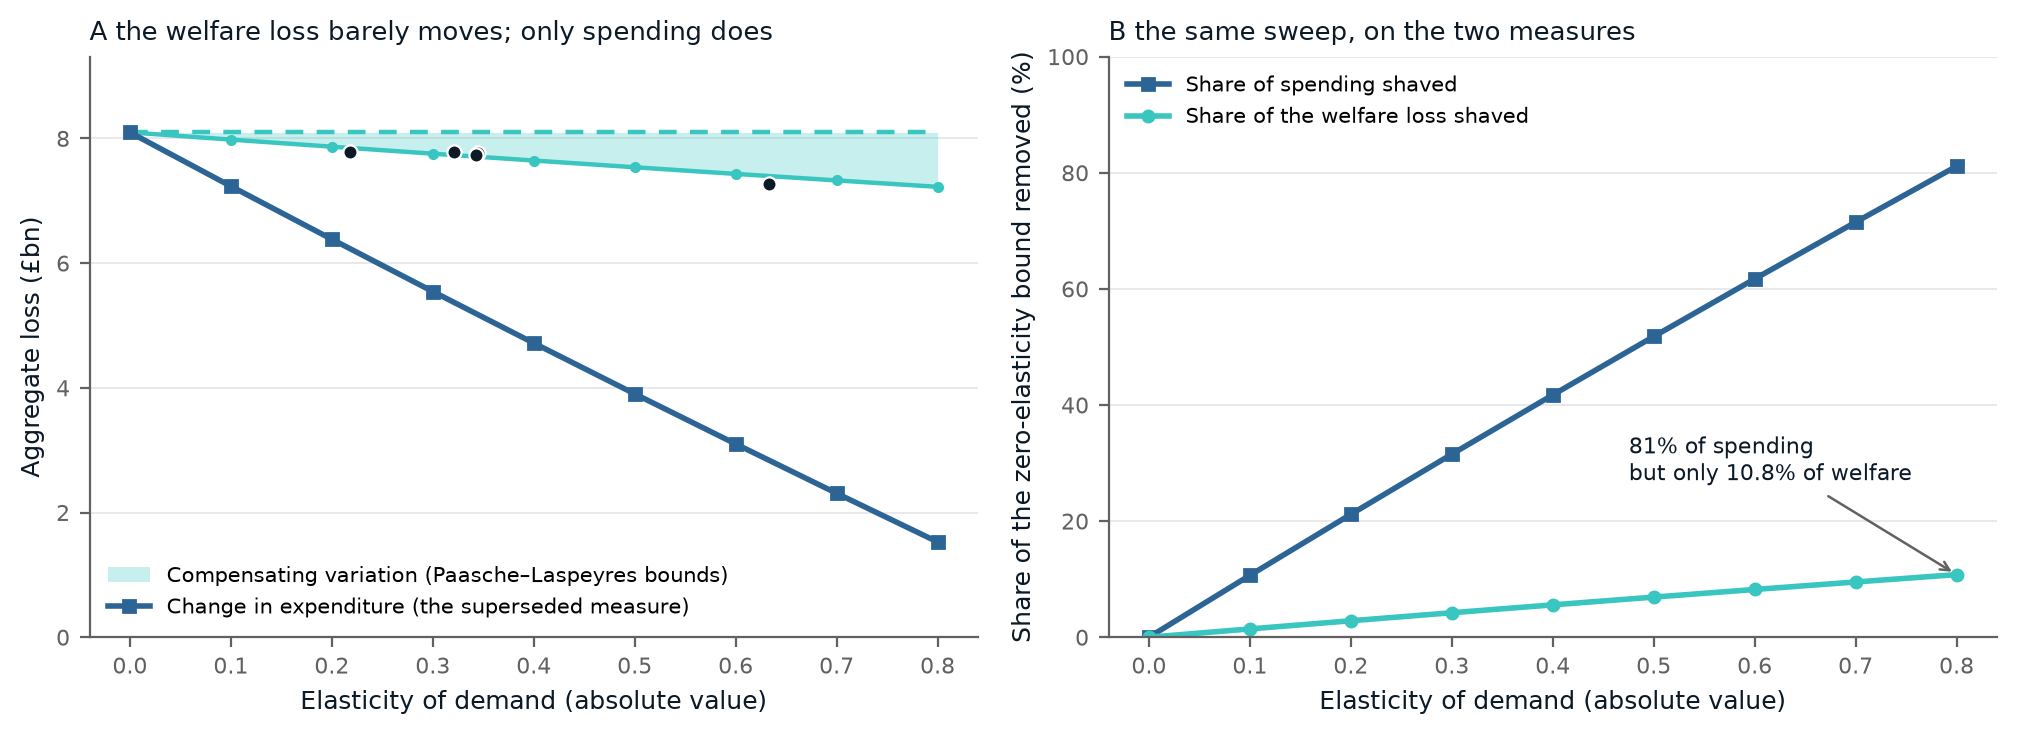
\includegraphics[width=\textwidth]{../results/figures/figA2_welfare_bounds.png}
\caption{Why the demand-response sweep is not the paper's largest uncertainty. Panel A places the change in expenditure --- the measure an earlier draft reported as the loss --- inside the Paasche--Laspeyres bounds on the compensating variation. Panel B shows the two on the same scale: at the strongest response in the grid, four fifths of the \emph{spending} disappears and about a tenth of the \emph{welfare loss} does. The difference is foregone consumption the household valued.}
\label{fig:welfarebounds}
\end{figure}

% tab_elasticity.tex — machine-generated by analysis/emit_tables.py
% generated 2026-08-26T12:16:39Z from results/ (central scenario: realised_2026). DO NOT EDIT BY HAND.
% A complete table float, caption and label included: the appendix inputs this directly. Requires \usepackage{booktabs}.
\begin{table}[htbp]
\centering
\caption{Demand-response sweep, realised 2026 scenario. The main specification is zero elasticity, an explicit upper bound on the welfare loss; every other row is a robustness check, not an alternative headline. The level of the loss moves by a factor of five across the grid; the qualitative decile ordering does not move at all.}
\label{tab:elasticity}
\begin{tabular}{lrrrrrr}
\toprule
Specification & Mean $\varepsilon$ & Mean loss (\pounds) & \% of income & Aggregate (\pounds bn) & Decile 1 (\%) & Decile 10 (\%) \\
\midrule
Labandeira et al., short run & $-$0.22 & 344 & 0.57 & 10.15 & 1.51 & 0.26 \\
Labandeira et al., long run & $-$0.63 & 134 & 0.22 & 3.94 & 0.58 & 0.10 \\
Priesmann and Praktiknjo, short run & $-$0.32 & 320 & 0.53 & 9.42 & 1.05 & 0.29 \\
Priesmann and Praktiknjo, long run & $-$0.34 & 314 & 0.52 & 9.25 & 1.08 & 0.28 \\
Prior-repository replication & $-$0.34 & 304 & 0.50 & 8.95 & 0.70 & 0.32 \\
Flat $\varepsilon = 0$ (main specification) & 0.00 & 471 & 0.77 & 13.89 & 2.07 & 0.36 \\
Flat $\varepsilon = -0.1$ & $-$0.10 & 420 & 0.69 & 12.36 & 1.84 & 0.32 \\
Flat $\varepsilon = -0.2$ & $-$0.20 & 369 & 0.61 & 10.87 & 1.62 & 0.28 \\
Flat $\varepsilon = -0.3$ & $-$0.30 & 319 & 0.53 & 9.42 & 1.40 & 0.24 \\
Flat $\varepsilon = -0.4$ & $-$0.40 & 271 & 0.45 & 7.99 & 1.19 & 0.21 \\
Flat $\varepsilon = -0.5$ & $-$0.50 & 223 & 0.37 & 6.59 & 0.98 & 0.17 \\
Flat $\varepsilon = -0.6$ & $-$0.60 & 177 & 0.29 & 5.21 & 0.78 & 0.14 \\
Flat $\varepsilon = -0.7$ & $-$0.70 & 131 & 0.22 & 3.87 & 0.58 & 0.10 \\
Flat $\varepsilon = -0.8$ & $-$0.80 & 87 & 0.14 & 2.55 & 0.38 & 0.07 \\
\bottomrule
\end{tabular}
\end{table}


\begin{figure}[htbp]
\centering
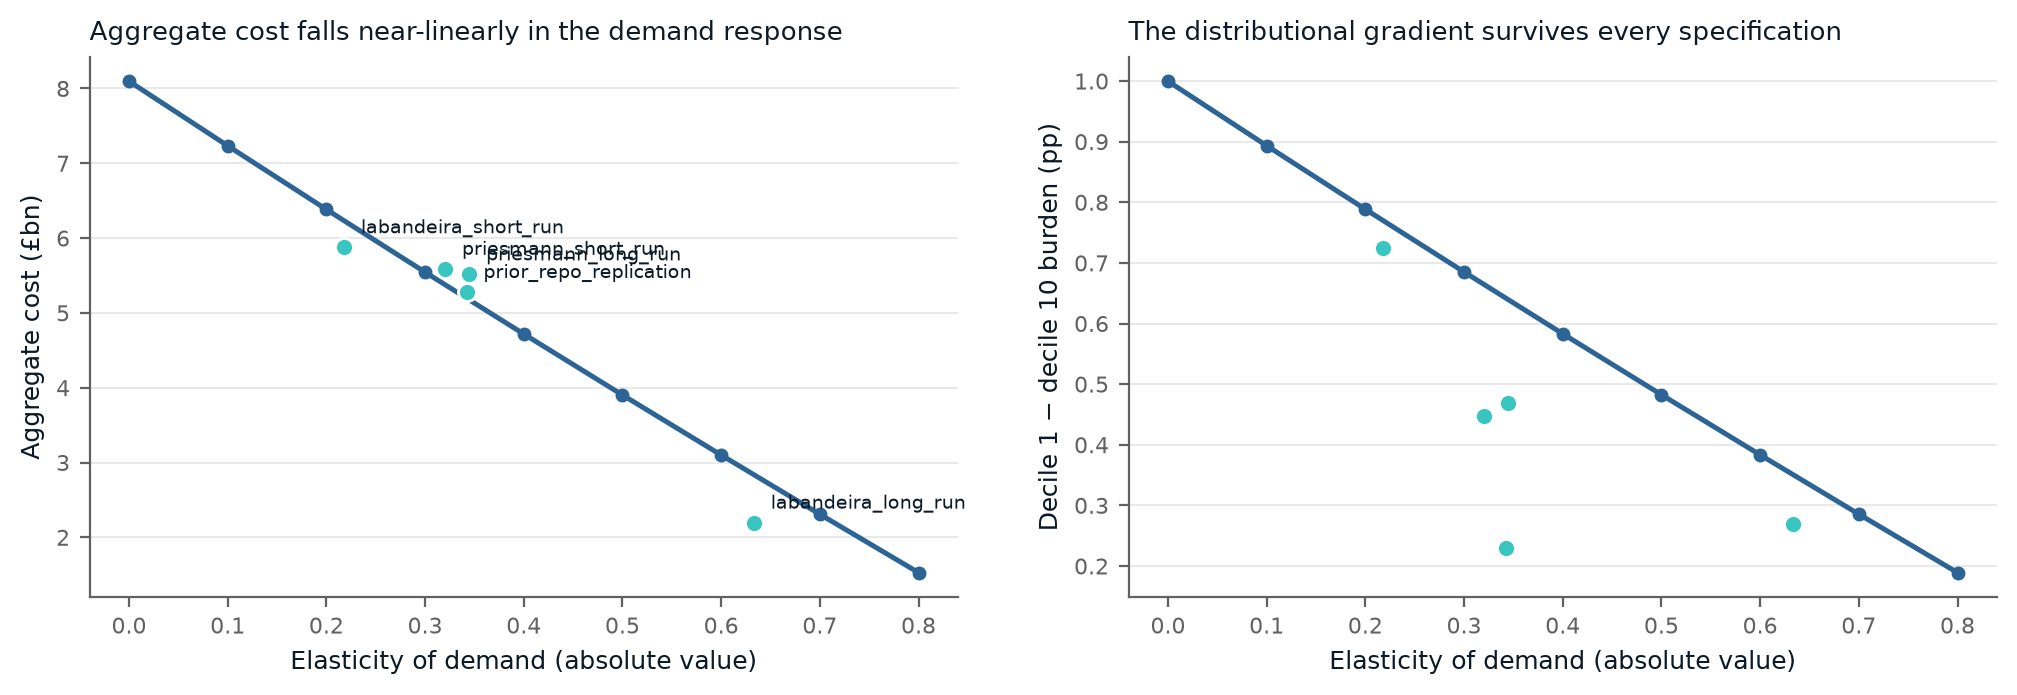
\includegraphics[width=.85\textwidth]{../results/figures/figA1_elasticity.png}
\caption{Decile incidence profile under each elasticity specification. The parallel spacing of the flat-grid lines shows that the distributional conclusions are invariant to a uniform elasticity assumption even where the level of the loss is not; the income-varying specifications flatten the gradient, for the reason discussed in the text.}
\label{fig:elasticity}
\end{figure}

A caveat on the exercise itself: applying a constant elasticity to a capped price is not innocuous, because households facing a standing charge plus a unit rate face a marginal price that differs from their average price, and the block designs scored in Section~\ref{sec:policy} change the marginal price for some households and not others. The sweep is fed the same bill factor as the main specification, not a unit rate --- an earlier version of this appendix claimed the latter --- and it does not model standing-charge effects, which would make the marginal price move by more than the bill does.

\subsection{Specification variants of the central scenario}
\label{app:specvariants}

Seven calibrations of the realised 2026 scenario are carried through the paper rather than one, and this subsection states what separates them so that any figure quoted in the text can be located. Table~\ref{tab:specifications} reports them on a common set of statistics. All seven are annualised over the same window, March 2026 to February 2027; none is a calendar-year figure.

The single statistic the seven are carried for is the motor-fuel share of the aggregate loss, and the range is the result rather than any point in it. Setting the peak-fuel upper bound aside --- it is a bound, not a candidate headline --- the share runs from \genSymDampMotorFuelShareOfLoss{} per cent under symmetric damping to \genMotorFuelShareOfLoss{} per cent in the main specification, with the ONS-levels calibration at \genOnsLevelsMotorFuelShareOfLoss{} per cent in between; including the peak-fuel row takes the top of the range to \genSpecFuelShareMaxPct{} per cent. The paper quotes the range. Motor fuel carries a large share on every calibration and a majority on most of them, and \genMotorFuelShareOfLoss{} per cent is not offered as settled.

\begin{table}[htbp]
\centering
\caption{The seven calibrations of the realised 2026 scenario, on a common set of statistics. The main specification applies the equivalised after-housing-costs denominator and the consumption-weighted quarterly cap average; each of the others varies one accounting or imputation choice from it.}
\label{tab:specifications}
% tab_specifications.tex — machine-generated by analysis/emit_tables.py
% generated 2026-08-27T09:07:01Z from results/ (central scenario: realised_2026). DO NOT EDIT BY HAND.
% A standalone tabular: \input this inside a table float that carries the caption and label. Requires \usepackage{booktabs}.
{\small\setlength{\tabcolsep}{2.6pt}
\begin{tabular}{lrrrrrrrrr}
\toprule
Specification & \begin{tabular}[b]{@{}c@{}}Agg. \\ (\pounds bn)\end{tabular} & \begin{tabular}[b]{@{}c@{}}Mean \\ (\pounds)\end{tabular} & \begin{tabular}[b]{@{}c@{}}Mean \\ (\%)\end{tabular} & \begin{tabular}[b]{@{}c@{}}D1 \\ (\pounds)\end{tabular} & \begin{tabular}[b]{@{}c@{}}D1 \\ (\%)\end{tabular} & \begin{tabular}[b]{@{}c@{}}D10 \\ (\pounds)\end{tabular} & \begin{tabular}[b]{@{}c@{}}D10 \\ (\%)\end{tabular} & \begin{tabular}[b]{@{}c@{}}D1/D10 \\ (\%)\end{tabular} & \begin{tabular}[b]{@{}c@{}}Motor fuel \\ (\% of loss)\end{tabular} \\
\midrule
Main specification & 8.10 & 275 & 0.60 & 231 & 2.29 & 314 & 0.25 & 9.22 & 75.6 \\
Steady state & 8.59 & 292 & 0.64 & 245 & 2.44 & 333 & 0.26 & 9.22 & 71.3 \\
Symmetric damping & 12.57 & 427 & 0.94 & 354 & 3.59 & 490 & 0.39 & 9.25 & 48.7 \\
Peak fuel (upper bound) & 11.39 & 387 & 0.85 & 326 & 3.22 & 441 & 0.35 & 9.21 & 82.7 \\
ONS shape & 8.13 & 276 & 0.61 & 140 & 1.41 & 473 & 0.37 & 3.75 & 75.7 \\
ONS both levels & 7.52 & 255 & 0.56 & 140 & 1.43 & 417 & 0.33 & 4.32 & 64.9 \\
Unequivalised & 8.10 & 275 & 0.45 & 231 & 1.16 & 314 & 0.21 & 5.53 & 75.6 \\
\bottomrule
\end{tabular}
}

\end{table}


The \emph{main} specification takes the annual domestic price as the consumption-weighted average of the quarterly cap levels prevailing over the modelled window of March 2026 to February 2027, damps both the wholesale gas peak and the observed pump-price peak to annual averages at sustained fractions of \genGasSustainedFraction{} and \genPumpSustainedFraction{} per cent respectively, and divides every percentage by equivalised net income after housing costs. It gives an aggregate loss of \pounds \genAggSpendRealisedBn{} billion, a mean household loss of \pounds \genCentralLossMean{} (\genCentralLossPctIncome{} per cent of income), a motor-fuel share of \genMotorFuelShareOfLoss{} per cent, and a decile-one to decile-ten burden ratio of \genDecileRatioPct{} to one.

The \emph{steady-state} specification charges the level the cap eventually reaches for the whole of the modelled window rather than the phased-in average --- which is what the code did before this revision, in contradiction of the method the paper describes. It gives \pounds \genSteadyStateAggBn{} billion, \pounds \genSteadyStateLossMean{} (\genSteadyStateLossPctIncome{} per cent), a motor-fuel share of \genSteadyStateMotorFuelShareOfLoss{} per cent and a ratio of \genSteadyStateDecileRatioPct{} to one. It is reported because it is the specification the earlier draft's headline figures came from, and because it is a defensible answer to a different question --- what an indefinitely sustained shock would cost --- rather than to the twelve-months-from-the-shock question this paper asks.

The \emph{symmetric-damping} specification is the one that most threatens the paper's compositional claim, and it is reported for that reason. It damps the gas and pump peaks by a \emph{common} fraction rather than by the fuel-specific pair the main specification uses, which is what a reader unpersuaded by the argument in Section~\ref{sec:step1} would impose. It gives \pounds \genSymDampAggBn{} billion, \pounds \genSymDampLossMean{} (\genSymDampLossPctIncome{} per cent), a ratio of \genSymDampDecileRatioPct{} to one --- and a motor-fuel share of \genSymDampMotorFuelShareOfLoss{} per cent, which is a minority. Combined with the steady-state basis it gives \genSymDampSteadyMotorFuelShare{} per cent and combined with ONS-consistent spending levels \genSymDampOnsLevelsMotorFuelShare{} per cent. The motor-fuel share depends on the \emph{ratio} of the two damping fractions and on little else, so this single choice moves the composition result more than any other in the paper while leaving the distributional result untouched.

The \emph{peak-fuel} specification is the upper bound: it applies the observed peak pump prices undamped for a full year, giving \pounds \genPeakFuelAggBn{} billion, \pounds \genPeakFuelLossMean{} (\genPeakFuelLossPctIncome{} per cent), a motor-fuel share of \genPeakFuelMotorFuelShareOfLoss{} per cent, and a ratio of \genPeakFuelDecileRatioPct{} to one. It is not a candidate headline: charging households an annual average pump price equal to a peak that lasted part of the year is a larger shock than the one that occurred, not a bound on it.

\begin{table}[htbp]
\centering
\caption{The calibrations of the realised 2026 scenario compared: the main specification, the steady-state accounting basis, symmetric damping, the peak-fuel upper bound, the two ONS calibrations, and the unequivalised robustness line.}
\label{tab:variants}
% tab_variants.tex — machine-generated by analysis/emit_tables.py
% generated 2026-08-27T12:30:25Z from results/ (central scenario: realised_2026). DO NOT EDIT BY HAND.
% A standalone tabular: \input this inside a table float that carries the caption and label. Requires \usepackage{booktabs}.
{\small\setlength{\tabcolsep}{4.5pt}
\begin{tabular}{lrrrr}
\toprule
 & \begin{tabular}[b]{@{}c@{}}Main \\ specification\end{tabular} & \begin{tabular}[b]{@{}c@{}}Peak-fuel \\ upper bound\end{tabular} & \begin{tabular}[b]{@{}c@{}}ONS-calibrated \\ motor fuel\end{tabular} & \begin{tabular}[b]{@{}c@{}}Calendar 2026 \\ (RF window)\end{tabular} \\
\midrule
Aggregate additional spend (\pounds bn) & 11.10 & 14.39 & 11.13 & 9.13 \\
Mean loss (\pounds) & 377 & 488 & 378 & 310 \\
Mean loss (\% of income) & 0.83 & 1.07 & 0.83 & 0.68 \\
\midrule
Decile 1 loss (\pounds) & 313 & 409 & 222 & 259 \\
Decile 1 loss (\% of income) & 3.16 & 4.09 & 2.27 & 2.60 \\
Decile 10 loss (\pounds) & 432 & 559 & 591 & 355 \\
Decile 10 loss (\% of income) & 0.34 & 0.44 & 0.47 & 0.28 \\
Decile 1/10 ratio (\% of income) & 9.24 & 9.23 & 4.86 & 9.23 \\
\quad from decile 2 (D2/D10) & 4.46 & 4.31 & 3.01 & 4.37 \\
\quad D1/D10, winsorised & 11.42 & 11.49 & 5.92 & 11.46 \\
\quad D2/D10, winsorised & 4.51 & 4.35 & 3.04 & 4.42 \\
\midrule
Gas share of loss (\%) & 24.8 & 19.1 & 24.7 & 20.9 \\
Electricity share of loss (\%) & 20.1 & 15.5 & 20.0 & 18.0 \\
Motor fuel share of loss (\%) & 55.2 & 65.4 & 55.3 & 61.0 \\
\midrule
Means-tested share of loss (\%) & 5.22 & 4.59 & 4.91 & 4.85 \\
\bottomrule
\end{tabular}
}

\end{table}

The two \emph{ONS} specifications address the imputation defects of Section~\ref{sec:limitations}. The first rescales the decile \emph{shape} of motor-fuel spending to the ONS Family Spending FYE 2025 profile. The rescaling preserves the microdata's national total and transplants only the ONS shape, so the rescaled decile levels --- \pounds \genRescaledFuelDecileOneGbp{} at the bottom against \pounds \genRescaledFuelDecileTenGbp{} at the top --- sit well above the ONS levels whose shape they borrow (\pounds \genOnsBenchFuelDecileOneGbp{} and \pounds \genOnsBenchFuelDecileTenGbp{}); an earlier draft quoted the rescaled figures three times as though they were the ONS benchmark, and they are not. Correcting the shape alone: it barely moves the aggregate, at \pounds \genOnsFuelAggBn{} billion and \pounds \genOnsFuelLossMean{} (\genOnsFuelLossPctIncome{} per cent) with a motor-fuel share of \genOnsFuelMotorFuelShareOfLoss{} per cent, and moves the distribution a great deal: decile one falls from \genDecileOneLossPct{} to \genOnsFuelDecileOneLossPct{} per cent of income, decile ten \emph{rises} from \genDecileTenLossPct{} to \genOnsFuelDecileTenLossPct{} per cent (in cash, from \pounds \genDecileTenLossGbp{} to \pounds \genOnsFuelDecileTenLossGbp{}), and the ratio falls to \genOnsFuelDecileRatioPct{} to one. The second corrects both spending \emph{levels} as well --- motor fuel down, domestic energy up --- giving \pounds \genOnsLevelsAggBn{} billion, \pounds \genOnsLevelsLossMean{} (\genOnsLevelsLossPctIncome{} per cent), a motor-fuel share of \genOnsLevelsMotorFuelShareOfLoss{} per cent and a ratio of \genOnsLevelsDecileRatioPct{} to one. Together they are the relevant robustness tests for every distributional magnitude in the paper, and the reason those magnitudes are reported as uncertain by roughly a factor of two.

The \emph{unequivalised} line is not an alternative specification but a visibility device. Dividing by raw household net income rather than by equivalised net income after housing costs --- which is what the code did before this revision, while the text claimed otherwise --- gives a mean burden of \genUnequivLossPctIncome{} per cent, a decile-one burden of \genUnequivDecileOneLossPct{} per cent against \genUnequivDecileTenLossPct{} per cent in decile ten, and a ratio of \genUnequivDecileRatioPct{} to one against \genDecileRatioPct{} on the equivalised basis. It is reported once so that the effect of the correction can be seen rather than inferred.

\subsection{Cap lag: a real sensitivity, now small}
\label{app:caplag}

The lag $\ell$ in equation~\eqref{eq:passthrough} places the quarterly phase-in profile on the calendar. It is the paper's most contestable calibration, so it is swept over one to four quarters against the loss annualised on the paper's own window --- March 2026 to February 2027 --- and the sweep is the paper's reconciliation as well as its sensitivity check. The domestic-energy channel is lagged; motor fuel is not, because pump prices pass through in weeks.

Two things about this subsection have changed, and the first is structural. The phase-in profile is now computed \emph{from} $\ell$ rather than written down as a fixed tuple alongside it. Previously the two were disconnected: the cumulative weight applied to the profile carried no lag dependence at all, so the invariance this appendix reported was an identity of the construction rather than a finding about the world, and the same disconnection was what allowed the headline and this sweep to disagree by roughly half. The profile now follows the lag, the sweep asserts that its central row reproduces the headline exactly, and the invariance it reports is therefore a measured residual rather than a guaranteed zero.

\paragraph{What the sweep now finds.} The mean household loss runs from \pounds\genCapLagAnnualisedLagOne{} at $\ell = 1$ to \pounds\genCapLagAnnualisedLagFour{} at $\ell = 4$, with the paper's $\ell = 1.5$ giving \pounds\genCapLagAnnualisedPaper{} --- which is the headline figure of \pounds \genCentralLossMean{}, by assertion rather than by coincidence. The spread across the whole range is \pounds \genCapLagRangeGbp{} per household, \genCapLagSpreadPct{} per cent of the central figure. That is a real sensitivity and a small one, and the reason it is small is the window: with both legs annualised over the twelve months from the shock, a shift in where the cap profile starts moves how much of the domestic pass-through falls inside a window that contains both cap resets either way. Under the earlier mismatched windows the same shift moved the answer by roughly fifty per cent, because a calendar-2026 window clipped the domestic leg exactly where the lag placed it.

\paragraph{Anchored against unanchored.} The sweep is run twice, and the pair is what shows how much of the small spread is the anchor doing its work. In the \emph{anchored} rows the gas sustained fraction is re-solved at each lag so that the modelled October cap continues to reproduce Ofgem's confirmed level \citep{ofgem2026cap} --- which is what the main specification does, since the fraction is solved rather than assumed (Section~\ref{sec:step1}). In the \emph{unanchored} rows the fraction is held at its central value while the lag moves, so the modelled cap drifts away from the confirmed one. The anchored spread is \pounds \genCapLagRangeGbp{} (\genCapLagSpreadPct{} per cent); the unanchored spread is \pounds \genCapLagRangeUnanchoredGbp{} (\genCapLagSpreadUnanchoredPct{} per cent), roughly twice as wide, and it widens monotonically with the lag because a longer lag pushes more of the profile past the anchor quarter and the fraction is no longer free to compensate. The anchor is therefore not cosmetic: it absorbs about half the lag sensitivity by construction, and it does so by holding the one quantity in the domestic leg that is externally observed.

Two consequences for how the paper's numbers should be read. First, any annual figure in this paper is lag-sensitive by \genCapLagSpreadPct{} per cent, which is smaller than the specification spread of Appendix~\ref{app:specvariants} and much smaller than the imputation uncertainty, so the lag has moved from the top of the uncertainty ranking to near the bottom. Second, the composition still moves more than the level does: the motor-fuel share of the loss runs across the swept range in the same direction, because a longer lag defers domestic pass-through while the pump leg does not move, which is the same calibration dependence Section~\ref{sec:results-fuel} reports arriving here from a third direction.

% tab_caplag.tex — machine-generated by analysis/emit_tables.py
% generated 2026-08-27T09:07:01Z from results/ (central scenario: realised_2026). DO NOT EDIT BY HAND.
% A complete table float, caption and label included: the appendix inputs this directly. Requires \usepackage{booktabs}.
\begin{table}[htbp]
\centering
\caption{Wholesale-to-retail lag sweep, realised 2026 scenario, on both anchoring rules. ``Anchored'' re-solves the sustained fraction at each lag so the Cornwall cap anchor still binds; ``unanchored'' holds it at the central value and so varies the timing alone. The cumulative burden is invariant along the unanchored series --- an identity, since the phase-in weights only move the burden between calendar years --- so what moves in the columns below is the attribution to the modelled year, not the size of the shock. The two rules agree to two quarters and separate after, which is where the anchoring rule rather than the lag is doing the work.}
\label{tab:caplag}
{\small\setlength{\tabcolsep}{4.5pt}
\begin{tabular}{llrrrrr}
\toprule
& & \multicolumn{2}{c}{Booked in the modelled year} & \multicolumn{2}{c}{By leg (\pounds bn)} & \\
\cmidrule(lr){3-4} \cmidrule(lr){5-6}
\begin{tabular}[b]{@{}l@{}}Lag \\ (quarters)\end{tabular} & \begin{tabular}[b]{@{}l@{}}Cap \\ anchoring\end{tabular} & \begin{tabular}[b]{@{}c@{}}Mean \\ (\pounds)\end{tabular} & \begin{tabular}[b]{@{}c@{}}Total \\ (\pounds bn)\end{tabular} & Domestic & \begin{tabular}[b]{@{}c@{}}Motor \\ fuel\end{tabular} & \begin{tabular}[b]{@{}c@{}}Motor fuel \\ share (\%)\end{tabular} \\
\midrule
1 & anchored & 280 & 8.25 & 2.13 & 6.12 & 74.2 \\
 & unanchored & 280 & 8.25 & 2.13 & 6.12 & 74.2 \\
1.5 (paper) & anchored & 275 & 8.10 & 1.98 & 6.12 & 75.6 \\
 & unanchored & 275 & 8.10 & 1.98 & 6.12 & 75.6 \\
2 & anchored & 271 & 7.99 & 1.87 & 6.12 & 76.6 \\
 & unanchored & 271 & 7.99 & 1.87 & 6.12 & 76.6 \\
3 & anchored & 267 & 7.86 & 1.74 & 6.12 & 77.9 \\
 & unanchored & 263 & 7.76 & 1.64 & 6.12 & 78.9 \\
4 & anchored & 272 & 8.02 & 1.90 & 6.12 & 76.3 \\
 & unanchored & 253 & 7.47 & 1.35 & 6.12 & 82.0 \\
\bottomrule
\end{tabular}
}
\end{table}


\begin{figure}[htbp]
\centering
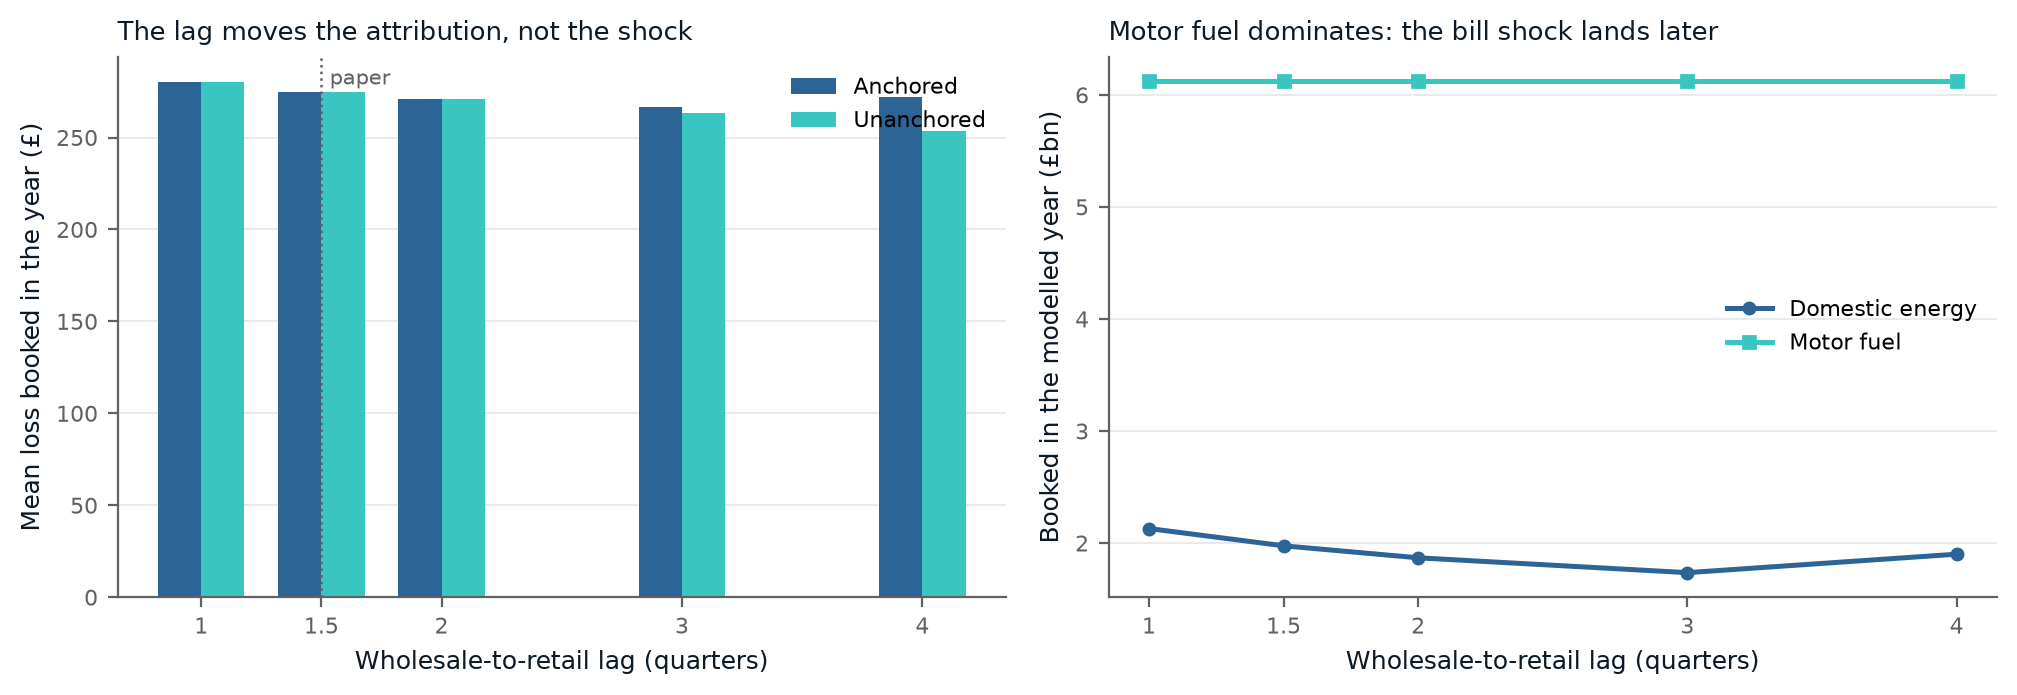
\includegraphics[width=.85\textwidth]{../results/figures/figA3_cap_lag.png}
\caption{Mean household loss over the modelled window under lags of one to four quarters, anchored and unanchored. The anchored series is the main specification's, with the gas sustained fraction re-solved at each lag against Ofgem's confirmed October cap; the unanchored series holds the fraction fixed. The gap between the two is how much of the lag sensitivity the anchor absorbs.}
\label{fig:caplag}
\end{figure}

\subsection{Marginal-pricing share: composition, not incidence}
\label{app:asymmetry}

The share of the time a gas-fired plant sets the GB marginal electricity price governs how far a wholesale gas move reaches the electricity cap. The main specification uses 0.85; setting it to 1.00 recovers the naive symmetric assumption that the move reaches electricity undamped, and 0.70 bounds it from below.

Stated plainly: it barely moves the answer. Going the whole way from 0.70 to 1.00 changes the mean household loss from \pounds\genAsymMeanLossLow{} to \pounds\genAsymMeanLossHigh{}, a difference of \genAsymMeanShiftPct{} per cent, and the decile-one to decile-ten percentage ratio is frozen at \genAsymRatioLow{} against \genAsymRatioHigh{} across the entire range. Nothing in the paper's distributional conclusions turns on this parameter, and Section~\ref{sec:step1} says so rather than claiming otherwise.

Where it does bite is composition, which is the one column that moves materially: the gas share of the domestic-energy loss falls from \genGasShareDomesticLow{} per cent at 0.70 to \genGasShareDomesticHigh{} per cent at 1.00, against \genGasShareDomesticCentral{} per cent in the main specification. Under the naive symmetric assumption the shock looks like an essentially even gas--electricity event; under the paper's calibration it is meaningfully gas-weighted. That matters for policy design and not for headline incidence: a gas-only social tariff, an electricity-side levy rebate, and the JRF block's choice of which unit rate to discount all land differently depending on which fuel carries the loss.

The honest summary is therefore narrow. The asymmetry is defensible on its merits and is the right modelling choice, but it is a compositional refinement rather than a load-bearing assumption. A reader who insists on the symmetric marginal-pricing assumption gets a mean loss \genAsymMeanShiftPct{} per cent larger and identical distributional conclusions. Note that this is the marginal-pricing share, not the gas-versus-pump damping ratio of Appendix~\ref{app:specvariants}: the first is a compositional refinement within the domestic leg, the second moves the motor-fuel share across the majority threshold. Confusing the two would understate how much of this paper's composition result is calibration.

% tab_asymmetry.tex — machine-generated by analysis/emit_tables.py
% generated 2026-08-26T13:05:57Z from results/ (central scenario: realised_2026). DO NOT EDIT BY HAND.
% A complete table float, caption and label included: the appendix inputs this directly. Requires \usepackage{booktabs}.
\begin{table}[htbp]
\centering
\caption{Marginal-pricing-share sweep, realised 2026 scenario. The gas price factor is held at 1.1404 throughout; only the electricity pass-through varies. The headline incidence barely moves, while the composition of the domestic loss moves materially.}
\label{tab:asymmetry}
{\small\setlength{\tabcolsep}{4.5pt}
\begin{tabular}{lrrrrrr}
\toprule
\begin{tabular}[b]{@{}l@{}}Marginal- \\ pricing share\end{tabular} & \begin{tabular}[b]{@{}c@{}}Electricity \\ factor\end{tabular} & \begin{tabular}[b]{@{}c@{}}Mean loss \\ (\pounds)\end{tabular} & \begin{tabular}[b]{@{}c@{}}Loss \\ (\% inc.)\end{tabular} & \begin{tabular}[b]{@{}c@{}}Decile \\ 1/10 ratio\end{tabular} & \begin{tabular}[b]{@{}c@{}}Gas share of \\ domestic loss (\%)\end{tabular} & \begin{tabular}[b]{@{}c@{}}Aggregate \\ (\pounds bn)\end{tabular} \\
\midrule
0.70 & 1.0764 & 331 & 0.54 & 5.68 & 59.3 & 9.76 \\
0.85 (paper) & 1.0928 & 343 & 0.56 & 5.68 & 54.6 & 10.12 \\
1.00 & 1.1092 & 356 & 0.58 & 5.67 & 50.5 & 10.48 \\
\bottomrule
\end{tabular}
}
\end{table}


\subsection{The scenario grid: when does the shock stop being a pump-price event?}
\label{app:grid}

The three named scenarios are points, and a reader is entitled to ask how much of the paper's argument is an artefact of where those points happen to sit. Figure~\ref{fig:grid} answers that by sweeping the two drivers against each other: a wholesale gas move, which reaches households through the regulated cap, against a crude oil move, which reaches them at the pump. Every cell is built through the same pass-through machinery as the named scenarios and scored on the same baseline, so the grid is a genuine extension of the main specification rather than a separate exercise.

\begin{figure}[htbp]
\centering
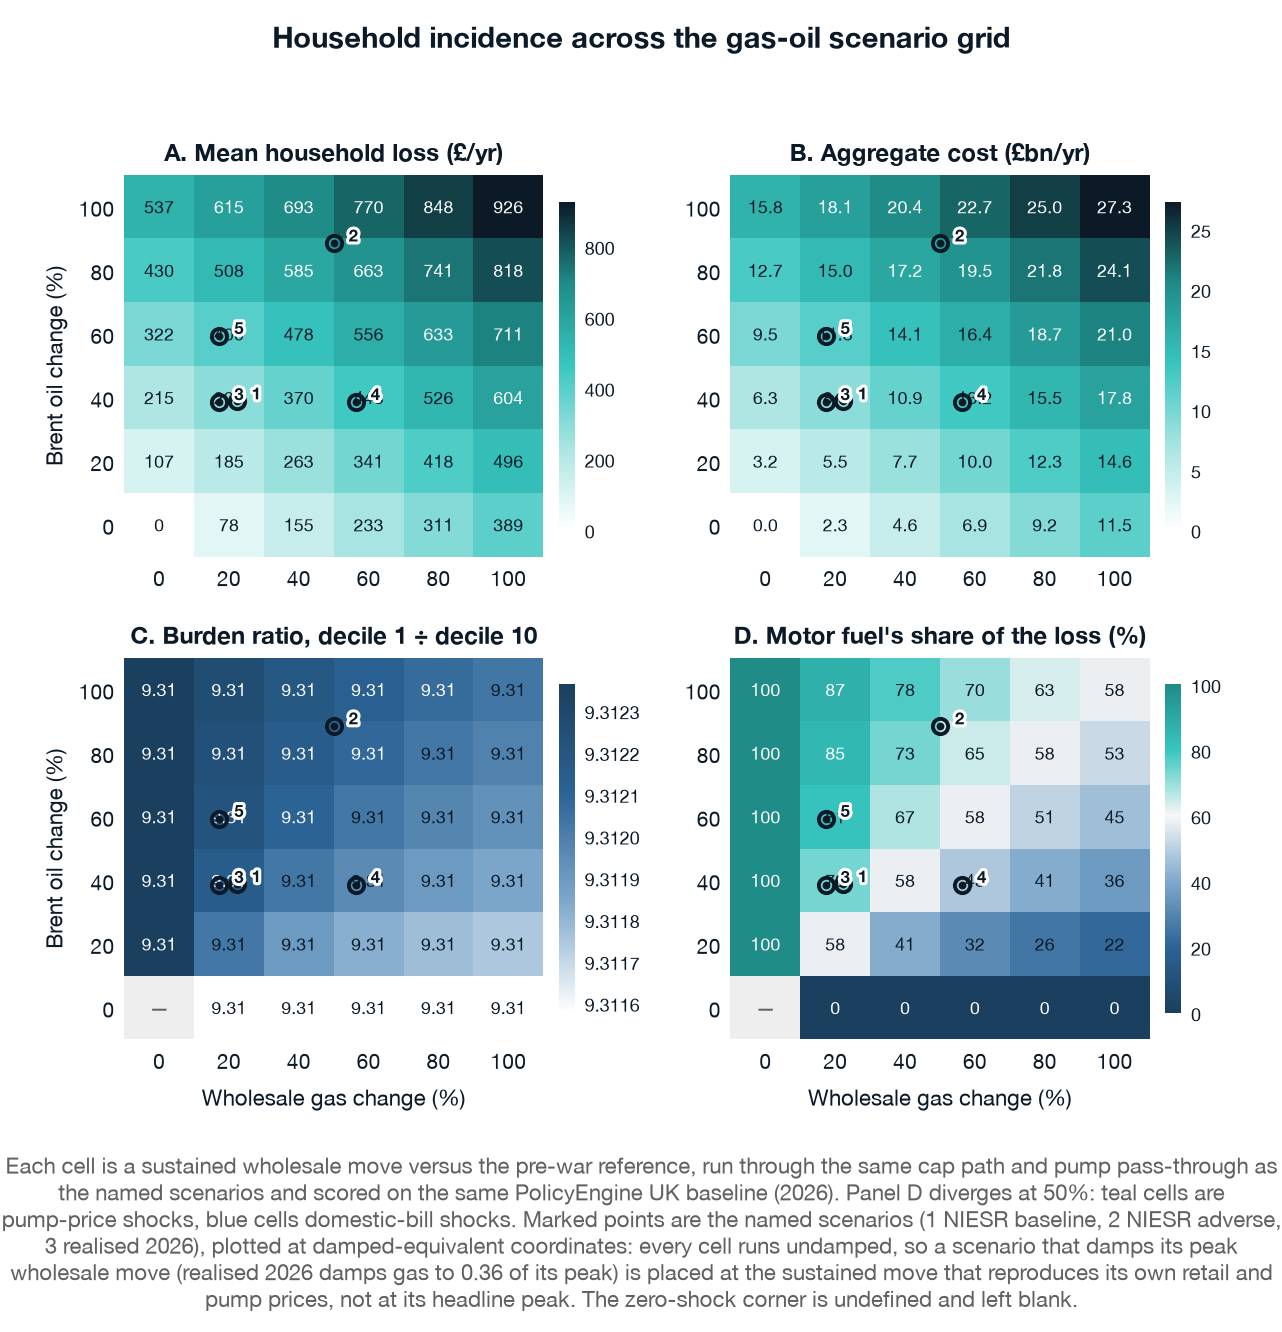
\includegraphics[width=\textwidth]{../results/figures/fig_scenario_grid.png}
\caption{Household incidence across the gas--oil scenario grid. Panel D diverges at fifty per cent: shaded one way the shock is a pump-price event, the other a domestic-bill event. Marked points are the three named scenarios.}
\label{fig:grid}
\end{figure}

One correction has to come before the results, because an earlier version of this appendix reported grid decile ratios that no reader could reconcile with the rest of the paper. The published grid gave decile-one to decile-ten burden ratios of 11.77 to 12.73, outside the range of every specification in the paper, with no reconciliation offered. Those figures were a stale artefact: they were computed on the unequivalised denominator this revision replaces (Section~\ref{sec:step2}), while the named scenarios had already moved to the equivalised one. Regenerated on the paper's own denominator, every cell of the grid returns \genDomesticOnlyDecileRatioPct{} to one, consistent with the domestic-only ratio the named scenarios produce. The consistency is now enforced rather than asserted: the burden ratio is an aggregate ratio and therefore scale-invariant, so a named scenario differs from a grid cell only in its channel mix and any mix must produce a ratio bracketed by the two pure-channel cells. \texttt{run\_grid.py} checks every named scenario against the live grid's range and \emph{raises} if one falls outside it, so a grid and a headline produced by different code cannot both be published again.

Two things follow. The first is that the distributional gradient is invariant to the mix. The decile-one to decile-ten burden ratio moves only between \genGridRatioMin{} and \genGridRatioMax{} across the entire grid, so the paper's central finding --- that the burden falls steeply in income even where the cash loss does not --- does not depend on which driver carries the shock. That near-degeneracy is itself informative rather than reassuring: the domestic and motor-fuel channels turn out to have almost the same decile gradient in this imputation, which is the fuel-imputation defect of Section~\ref{sec:limitations} --- deciles one and ten recording the same fuel-purchasing rate --- showing up from a different direction. The gradient is a property of how the imputed energy and fuel budget shares vary with income, and the flatness of the grid is a reminder that one of those two profiles is known to be wrong.

The second is a boundary. Motor fuel ceases to carry the larger share of the loss along a frontier at roughly \genGridFrontierSlope{} times as large a proportional gas move as oil move; below that line the shock is predominantly a pump-price event and above it predominantly a domestic-bill one. One caution about reading the named scenarios against that frontier: every cell of the grid is run undamped, and the named scenarios are plotted at their undamped coordinates, so the comparison is not like-for-like with the damped main specification whose motor-fuel share Section~\ref{sec:results-fuel} reports. An earlier version of this appendix asserted that all three named scenarios sit below the frontier; on the grid's own undamped numbers that is not established, and the claim is withdrawn. What the grid does show is that the frontier exists, that it is not far from the region a gas-and-oil shock of this kind occupies, and that which side of it a given shock falls on depends on the damping calibration --- which is the same calibration dependence Section~\ref{sec:results-fuel} reports, arriving here from a different direction.


\subsection{The common exchequer envelope, and its four row types}
\label{app:envelope}

Table~\ref{tab:envelope} reports every instrument at each of the four row types set out in Section~\ref{sec:step4}: at the sponsor's own stated cost, at the instrument's feasible maximum, at a parameter scaled past that maximum until the \pounds \genEnvelopeBn{} billion envelope is exhausted, and at widened eligibility with generosity held at the sponsor's own parameter. Each row carries a feasibility flag and, where the instrument cannot absorb the envelope, the amount it can absorb.

The table is the arithmetic behind the withdrawal in Section~\ref{sec:policy}. VAT zero-rating absorbs \pounds \genVatCutCostBn{} billion --- the whole of the five-point reduced rate --- so its feasible-maximum row and its stated-cost row coincide and no scaling makes it a \pounds \genEnvelopeBn{} billion instrument; the social tariff absorbs \pounds \genSocialTariffAbsorbableBn{} billion and the Warm Home Discount expansion \pounds \genWhdAbsorbableBn{} billion. The three scaled rows that exceed a feasible maximum are labelled generically --- a proportional domestic-bill subsidy at \genSocialTariffScaledParameterPct{} per cent on the means-tested population, a flat payment of \pounds \genWhdScaledParameterGbp{} a year to the same population, and a proportional domestic-bill subsidy at \genVatCutScaledParameterPct{} per cent universally --- because none of them is the policy whose name it used to carry. The eligibility rows are feasible throughout, and the comparison between them and the feasible-maximum rows is the finding of Section~\ref{sec:policy-eligibility}.

\begin{figure}[htbp]
\centering
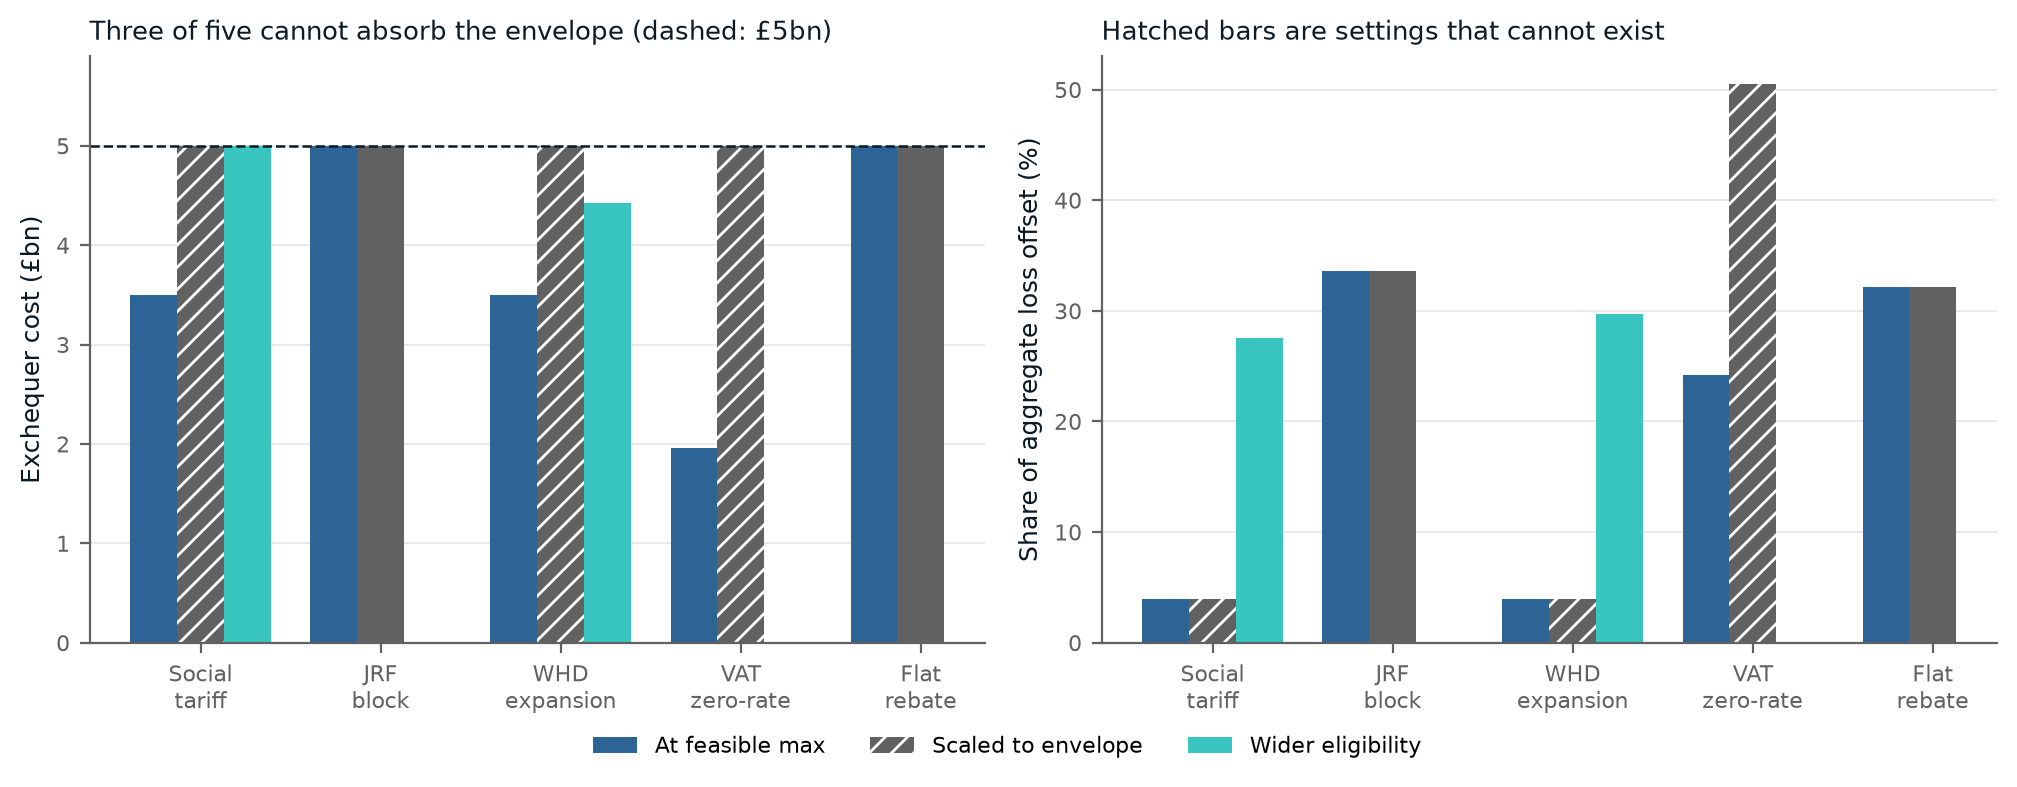
\includegraphics[width=\textwidth]{../results/figures/figA4_policy_envelope.png}
\caption{The five instruments at a common exchequer envelope. Rows whose implied parameter does not exist are marked: the ranking they generate is not a ranking of the policies named. Widening eligibility at each sponsor's own generosity offsets far more of the loss than deepening the discount at fixed eligibility.}
\label{fig:envelope}
\end{figure}

% tab_envelope.tex — machine-generated by analysis/emit_tables.py
% generated 2026-08-27T11:36:28Z from results/ (central scenario: realised_2026). DO NOT EDIT BY HAND.
% A complete table float, caption and label included: the appendix inputs this directly. Requires \usepackage{booktabs}.
\begin{table}[htbp]
\centering
\caption{The five instruments against a common exchequer envelope of \pounds 5bn, realised 2026 scenario. The first two rows for each instrument answer different questions and the pre-revision table conflated them. ``Own ceiling'' is the instrument at its own feasible maximum with no envelope applied at all: the JRF block reaches \pounds 21.9bn there, more than 4 times the envelope. ``Absorbs envelope'' is the budget constraint --- the smaller of the envelope and that ceiling --- so for an instrument that already costs more than \pounds 5bn it scales generosity \emph{down}, and for the three that saturate below the envelope it reports the smaller sum they can actually spend. Neither row holds spend fixed across instruments. ``Scaled'' is proportional scaling to the full envelope regardless of feasibility; $\dagger$ marks the three rows whose implied setting does not exist (a bill discount above 100 per cent, more VAT points than the tax has). ``Wider eligibility'' spends the envelope on who is in the scheme rather than on how generous it is, at the sponsor's own rate, and is defined only for the two means-tested schemes; $\ddagger$ marks the four such rows where widening reaches every household, at which point the instrument is means-tested in name only. Any claim that one instrument ``wins at a common envelope'' rests on the scaled rows and is withdrawn.}
\label{tab:envelope}
{\small\setlength{\tabcolsep}{2.6pt}
\begin{tabular}{llrrrrrr}
\toprule
Instrument & Variant & \begin{tabular}[b]{@{}c@{}}Spend \\ (\pounds bn)\end{tabular} & \begin{tabular}[b]{@{}c@{}}Implied \\ setting\end{tabular} & \begin{tabular}[b]{@{}c@{}}Share to \\ D1--3 (\%)\end{tabular} & \begin{tabular}[b]{@{}c@{}}Loss \\ offset (\%)\end{tabular} & \begin{tabular}[b]{@{}c@{}}Mean res- \\ idual (\pounds)\end{tabular} & \begin{tabular}[b]{@{}c@{}}Un-comp- \\ ensated (\%)\end{tabular} \\
\midrule
Social tariff & own ceiling & 3.76 & 100\% & 57.5 & 5.2 & 357 & 84 \\
 & absorbs envelope & 3.76 & 100\% & 57.5 & 5.2 & 357 & 84 \\
 & scaled & 5.00 & 133\%$^\dagger$ & 57.5 & 5.2 & 357 & 84 \\
 & wider eligibility & 5.00 & 35\% & 71.7 & 26.6 & 276 & 62 \\
\addlinespace
JRF block & own ceiling & 21.86 & 100\% & 29.7 & 70.5 & 111 & 10 \\
 & absorbs envelope & 5.00 & 22.9\% & 29.7 & 36.1 & 241 & 41 \\
 & scaled & 5.00 & 22.9\% & 29.7 & 36.1 & 241 & 41 \\
\addlinespace
WHD expansion & own ceiling & 3.76 & \pounds 814 & 60.0 & 5.1 & 357 & 85 \\
 & absorbs envelope & 3.76 & \pounds 814 & 60.0 & 5.1 & 357 & 85 \\
 & scaled & 5.00 & \pounds 1,083$^\dagger$ & 60.0 & 5.2 & 357 & 84 \\
 & wider eligibility$^\ddagger$ & 4.42 & \pounds 150 & 30.0 & 29.3 & 266 & 49 \\
\addlinespace
VAT zero-rate & own ceiling & 2.11 & 5\% & 24.7 & 19.0 & 305 & 100 \\
 & absorbs envelope & 2.11 & 5\% & 24.7 & 19.0 & 305 & 100 \\
 & scaled & 5.00 & 11.9\%$^\dagger$ & 24.7 & 44.9 & 208 & 78 \\
\addlinespace
Flat rebate & own ceiling$^\ddagger$ & 5.39 & \pounds 183 & 30.0 & 33.2 & 251 & 43 \\
 & absorbs envelope$^\ddagger$ & 5.00 & \pounds 170 & 30.0 & 31.7 & 257 & 45 \\
 & scaled$^\ddagger$ & 5.00 & \pounds 170 & 30.0 & 31.7 & 257 & 45 \\
\bottomrule
\end{tabular}
}
\end{table}


\subsection{The domestic leg: what the anchor does and does not pin}
\label{app:domesticleg}

Table~\ref{tab:domesticleg} sweeps the parameters that scale the domestic channel one for one and are not otherwise identified. The gas sustained fraction and the phase-in weight at the anchor quarter enter the cap only as a product, so the confirmed-cap anchor pins the product and not the split; the sweep varies the split at a fixed product to show that the headline is insensitive to it. It also varies the three parameters the anchor does not touch --- the pre-war NBP gas price, and the wholesale shares of the gas and electricity bills --- which move the domestic leg proportionally and therefore move the motor-fuel share, between \genDomesticLegNbpFuelShareMinPct{} and \genDomesticLegNbpFuelShareMaxPct{} per cent on the pre-war gas price alone. That is the largest single-parameter movement in the composition result and it is why Section~\ref{sec:results-fuel} quotes a range.

% tab_domestic_leg.tex — machine-generated by analysis/emit_tables.py
% generated 2026-08-26T15:20:08Z from results/ (central scenario: realised_2026). DO NOT EDIT BY HAND.
% A complete table float, caption and label included: the appendix inputs this directly. Requires \usepackage{booktabs}.
\begin{table}[htbp]
\centering
\caption{Domestic-leg parameter sweep, realised 2026 scenario. The Cornwall Insight anchor identifies only the product of the sustained fraction and the first phase-in quarter, so the first block varies the split at a constant product; the remaining blocks vary the three parameters that scale the domestic channel one for one. The aggregate, and with it the motor-fuel share, is materially sensitive to this calibration.}
\label{tab:domesticleg}
{\small\setlength{\tabcolsep}{2.6pt}
\begin{tabular}{llrrrrrr}
\toprule
Parameter & \begin{tabular}[b]{@{}l@{}}Value\end{tabular} & \begin{tabular}[b]{@{}c@{}}Agg. \\ (\pounds bn)\end{tabular} & \begin{tabular}[b]{@{}c@{}}Mean \\ (\pounds)\end{tabular} & \begin{tabular}[b]{@{}c@{}}Mean \\ (\%)\end{tabular} & \begin{tabular}[b]{@{}c@{}}D1 \\ (\%)\end{tabular} & \begin{tabular}[b]{@{}c@{}}D10 \\ (\%)\end{tabular} & \begin{tabular}[b]{@{}c@{}}Motor fuel \\ (\% of loss)\end{tabular} \\
\midrule
Sustained fraction & 0.18 & 7.54 & 256 & 0.56 & 2.13 & 0.23 & 74.9 \\
 & 0.24 & 8.01 & 272 & 0.60 & 2.27 & 0.25 & 70.5 \\
 & 0.3 & 8.49 & 288 & 0.63 & 2.41 & 0.26 & 66.6 \\
 & 0.36 (paper) & 8.96 & 304 & 0.67 & 2.55 & 0.28 & 63.1 \\
 & 0.45 & 9.67 & 328 & 0.72 & 2.75 & 0.30 & 58.5 \\
 & 0.6 & 10.85 & 368 & 0.81 & 3.09 & 0.33 & 52.1 \\
 & 0.72 & 11.79 & 400 & 0.88 & 3.37 & 0.36 & 47.9 \\
\midrule
Pre-war NBP & 70 & 9.90 & 336 & 0.74 & 2.82 & 0.31 & 57.1 \\
 & 80 & 9.37 & 318 & 0.70 & 2.67 & 0.29 & 60.3 \\
 & 90 (paper) & 8.96 & 304 & 0.67 & 2.55 & 0.28 & 63.1 \\
 & 100 & 8.63 & 293 & 0.64 & 2.45 & 0.27 & 65.5 \\
 & 110 & 8.36 & 284 & 0.62 & 2.37 & 0.26 & 67.6 \\
 & 130 & 7.94 & 269 & 0.59 & 2.25 & 0.24 & 71.2 \\
\midrule
Wholesale share, gas & 0.35 & 8.56 & 291 & 0.64 & 2.43 & 0.26 & 66.0 \\
 & 0.4 & 8.76 & 297 & 0.65 & 2.49 & 0.27 & 64.5 \\
 & 0.45 (paper) & 8.96 & 304 & 0.67 & 2.55 & 0.28 & 63.1 \\
 & 0.5 & 9.15 & 311 & 0.68 & 2.60 & 0.28 & 61.7 \\
 & 0.55 & 9.35 & 317 & 0.70 & 2.66 & 0.29 & 60.4 \\
\midrule
Wholesale share, elec. & 0.25 & 8.52 & 289 & 0.63 & 2.42 & 0.26 & 66.3 \\
 & 0.3 & 8.74 & 297 & 0.65 & 2.48 & 0.27 & 64.7 \\
 & 0.35 (paper) & 8.96 & 304 & 0.67 & 2.55 & 0.28 & 63.1 \\
 & 0.4 & 9.18 & 311 & 0.68 & 2.61 & 0.28 & 61.6 \\
 & 0.45 & 9.39 & 319 & 0.70 & 2.67 & 0.29 & 60.1 \\
\bottomrule
\end{tabular}
}
\end{table}


\subsection{Upstream contributions arising}
\label{app:upstream}

Three of this paper's limitations are model gaps rather than data gaps, and each is precise enough to fix. They are contributed upstream to PolicyEngine UK rather than only reported here: a live price channel for the imputed energy variables, so that a cap or pump-price reform moves household spend rather than silently cutting quantities; a Warm Home Discount parameter and variable, which the model currently lacks entirely; and a primary-heating-fuel or gas-grid indicator in the microdata, without which the off-gas-grid question in Section~\ref{sec:discussion} cannot be asked of any UK microsimulation.

Three calibration findings from this paper's validation work are contributed alongside them, because both are properties of the model rather than of this application. The first is the motor-fuel imputation: the imputed decile profile of motor-fuel spend is almost flat, \pounds \genFuelSpendDecileOneRawGbp{} against \pounds \genFuelSpendDecileTenRawGbp{}, where the ONS Family Spending profile runs \pounds \genOnsBenchFuelDecileOneGbp{} to \pounds \genOnsBenchFuelDecileTenGbp{} \citep{ons2026familyspending}, both annualised at $365.25/7 = 52.18$ weeks rather than at 52, and the fuel-purchasing participation rate is identical in deciles one and ten where the Department for Transport's National Travel Survey table on household car \emph{availability} shows 40 per cent of the poorest quintile without a car against 14 per cent of the richest \citep{dft2025nts} --- a table covering England only, while the model is UK-wide, so it bounds the direction of the defect rather than measuring it. The second is domestic energy, imputed in the opposite direction: mean modelled domestic spend of \pounds \genModelDomesticMeanGbp{} against ONS Family Spending's \pounds \genOnsBenchDomesticMeanGbp{} \citep{ons2026familyspending} and DESNZ's fixed-consumption dual-fuel bill \citep{desnz2026qep}, roughly a quarter low, and below the typical-consumption cap level, which a population mean should not be. The two run opposite ways and compound on the fuel share, so they are reported together. The third is means-tested coverage: the model's entire means-tested population, \genMeansTestedHouseholdsM{} million households, sits well below the 7.2 million households on Universal Credit alone in May 2026. All three are quantified against published administrative and survey benchmarks and are reported upstream in that form. The contributed energy-bills parameter that no variable reads is separately flagged for removal or implementation.

\subsection{Reproduction}
\label{app:reproduce}

This subsection is the one place in the paper where implementation detail is given, because reproduction requires it.

All code, parameters and aggregate results are in the paper's public repository; the microdata are not. PolicyEngine UK's enhanced Family Resources Survey dataset is held in a private repository under a licence that does not permit redistribution, so reproducing the household-level results requires an access token. The aggregate outputs are committed, so every number in the paper can be traced from the stored artefacts to the macro that renders it without re-running the microsimulation:

\begin{itemize}\setlength{\itemsep}{0pt}
  \item \texttt{analysis/run\_incidence.py} --- baseline, shock and policy scoring
  \item \texttt{analysis/run\_variants.py} --- the specification variants of Appendix~\ref{app:specvariants}
  \item \texttt{analysis/run\_sensitivity.py} --- the elasticity, cap-lag and marginal-pricing sweeps
  \item \texttt{analysis/run\_grid.py} --- the scenario grid of Figure~\ref{fig:grid}
  \item \texttt{analysis/emit\_tex\_values.py} --- every numeric macro used in the text
\end{itemize}
The model gaps recorded in Section~\ref{sec:limitations} correspond to open issues in the \texttt{policyengine-uk} repository: the absence of a demand-elasticity and pass-through block is issue \#1114, and the unvalidated 0.38 VAT coverage factor is issue \#352.

\begin{verbatim}
uv sync
export HUGGING_FACE_TOKEN=hf_...     # needs private dataset access
python analysis/run_incidence.py     # scenarios + policies -> results/*.json
python analysis/run_variants.py      # the seven specifications
python analysis/run_sensitivity.py   # the four sweeps
python analysis/run_grid.py          # scenario grid -> results/grid/*.csv
python analysis/emit_tables.py       # results/ -> paper/tables/*.tex
python analysis/emit_tex_values.py   # -> paper/values_generated.tex
python -m pytest tests/              # runs without microdata
cd paper && latexmk -pdf main.tex
\end{verbatim}

Every headline number enters the prose as a macro from \texttt{paper/values\_generated.tex}, emitted mechanically from \texttt{results/}. A macro with no corresponding key in \texttt{results/} renders as \texttt{\textbackslash GENMISSING}, so a stale or partial results tree fails visibly in the compiled document rather than silently preserving superseded numbers. This is also why no constituency-level or heating-fuel statistic appears anywhere in the paper: with no key in \texttt{results/} to back it, no such number can be rendered. Pinned dependency versions, including the \texttt{policyengine-uk} release used, are in \texttt{pyproject.toml} and \texttt{uv.lock}.


\end{document}
